\documentclass[aps,preprint,nofootinbib,preprintnumbers,eqsecnum,superscriptaddress]{revtex4}

\usepackage{amsmath} 
\usepackage{graphicx} 
\usepackage{amsthm}
\usepackage{amssymb} 
\usepackage{dsfont}
\usepackage{yfonts}

%\usepackage{floatrow,dcolumn,rotating}
\usepackage{array,xcolor,graphicx}
\usepackage{booktabs,multirow}
\usepackage{circuitikz}



\usepackage[utf8]{inputenc}
\usepackage{mathtools}

\usepackage{slashed}
\usepackage{caption}
\usepackage{stackrel}
\usepackage{cases}
\usepackage{tcolorbox}
%\usepackage{subcaption}

%ADDED BY ALESSIO
\usepackage{enumerate}
%END ADDITION BY ALESSIO

%Ensuring that header of section+subsection is on the right
\usepackage{etoolbox}
\patchcmd{\section}
  {\centering}
  {\raggedright}
  {}
  {}
\patchcmd{\subsection}
  {\centering}
  {\raggedright}
  {}
  {}
%

\usepackage[normalem]{ulem}
\usepackage{mathtools}


%package for drawing tool
\usepackage[all]{xy}
\usepackage{tikz}
\usetikzlibrary{arrows.meta}

\usepackage{hyperref}
%Set colour for the hyperlink
\hypersetup{colorlinks=true,linkcolor=blue,citecolor=red,urlcolor=blue, linktocpage=true}

%%%%%%%%%%%%%%%%%%%%%%%%%%%%%%%%%%%%%%%%%%%

\numberwithin{equation}{section}

% profondità di numerazione e TOC
\setcounter{secnumdepth}{3} % numerare fino alle subsubsection
\setcounter{tocdepth}{3}    % farle comparire nel TOC
% numerazione gerarchica: Part.Section.Subsection.Subsubsection
% Sezione: I.A
\renewcommand\thesection{\Roman{section}}
% Sottosezione: I.A.1
\renewcommand\thesubsection{\Roman{section}.\arabic{subsection}}
% Subsubsection: I.A.1.a (opzionale, cambia se vuoi un altro stile)
\renewcommand\thesubsubsection{\Roman{section}.\arabic{subsection}.\Alph{subsubsection}}

\makeatletter
\renewcommand{\p@section}{}        % niente prefisso per le section
\renewcommand{\p@subsection}{}     % niente prefisso per le subsection
\renewcommand{\p@subsubsection}{}  % niente prefisso per le subsubsection
\makeatother

\usepackage[]{mdframed}
\usepackage{mathtools}
\newcommand{\mycomment}[1]{}
%\usepackage{tikz-cd}
%\usetikzlibrary{arrows.meta}
%\usetikzlibrary{arrows}
\usepackage{tikz}
\usetikzlibrary{positioning}
\usepackage{float}
\newcommand{\figref}[1]{{FIG. \ref{#1}}}

\begin{document}

\title{Looking for Continuous Non-Invertible Symmetries\\in 3d Complex Scalar Boson}
\author{Alessio Martini} 
\email{alessio.martini@student.uva.nl}
\affiliation{Institute for Theoretical Physics, University of Amsterdam\\} 

\begin{abstract}
In this thesis, we study generalized global symmetries in quantum field theory, focusing on the 3D XY-model and its relation to the abelian Higgs model via particle-vortex duality. Our primary goal is to understand the nature of the emergent 1-form symmetry in the spontaneously symmetry broken (SSB) phase, and to investigate whether this infrared symmetry is already encoded as a non-invertible symmetry in the ultraviolet (UV) data. We show that the emergent symmetry cannot be captured as a non-invertible symmetry in the UV with the topological tools and frameworks currently available.

As our main original contribution, we provide an explicit extension of continuous non-invertible defects to general spacetime dimensions and arbitrary $p$-form degrees within mixed 't Hooft anomalies. Using the Symmetry TFT (SymTFT) framework we analyze four distinct scenarios. Scenarios 1 and 2 provide working methods to successfully generate continuous non-invertible symmetries on the boundary. Conversely, Scenarios 3 and 4 present cases where the method fails, serving as a clear proof of validity and mapping the exact boundaries of the framework. 
\end{abstract}
\maketitle


\tableofcontents

\newpage

%---------------------------------------------------------
\section{Introduction}
\label{sec:introduction}

The main goal of this master thesis is to study generalized symmetries in quantum field theory. In particular, we want to look at the 3D XY-model, which is related by particle-vortex duality to the abelian Higgs model, and understand the nature of the emergent 1-form symmetry in the spontaneously symmetry broken (SSB) phase. Our main question is whether this emergent symmetry is already encoded as a non-invertible symmetry in the UV data. The result of our work is that this emergent symmetry is not captured as a non-invertible symmetry in the UV, at least not in a way that we can study with the tools we used.

As the reader will notice, this thesis contains many interludes and side topics. These interludes are not strictly connected to the main line of the text, and they are not here to justify the construction. They are simply side topics that I found particularly interesting and entertaining during my past year of study, so I wanted to include them. Therefore, this thesis is a reflection of my one-year research journey, reorganized to try to create a logical flow using technicalities and curiosities in these interludes or boxes.

The main original result of this work is the explicit extension of these p-form symmetries to general dimensions and general form-degrees inside the anomaly polynomials when we build continuous non-invertible defects. This generalization was sometimes briefly hinted at in the literature, but here we provide the explicit construction and all the details.



\newpage
%---------------------------------------------------------
\section{Ordinary and generalized global symmetries}
%---------------------------------------------------------

Throughout this thesis we will discuss Generalized Global Symmetries, so it is necessary to clearly understand what we are discussing. Let us start from the following three basic questions:
\begin{enumerate}[1.]
    \item What is a symmetry?
    \item What does "generalized" mean in this context?
    \item What does "global" mean? Can we have a non-global symmetry?
\end{enumerate}

Let us give a brief overview now, followed by a detailed discussion immediately after.

The answer to the first question can be summarized as: "a symmetry is a topological operator". More precisely, the existence of an ordinary symmetry in a Quantum Field Theory (in Euclidean signature) implies the existence of a $(d-1)$-dimensional topological operator:
\begin{equation}
    \text{Ordinary Symmetry} \implies \text{Topological Operator}
\end{equation}

Anticipating the answer to the second question, we can invert and generalize this paradigm: whenever we find a topological operator in a Field Theory, we will define it as a Generalized Symmetry:
\begin{equation}
    \text{Generalized Symmetry} \iff \text{Topological Operator}
\end{equation}

This perspective generalizes two main features: the dimensionality of the topological operator (a $p$-form symmetry is associated with a topological operator whose support has dimension $d-p-1$), and the composition law when we overlay two symmetry operators (a non-invertible symmetry is associated with operators that do not follow a simple group law).

There are clear advantages to taking this modern perspective \cite{McGreevy_2023}:
\begin{enumerate}[\itshape i)]
    \item Continuous and discrete symmetries are treated uniformly within the same geometric framework.
    \item It makes no explicit reference to field transformations, putting standard Noether symmetries and purely topological symmetries on the exact same footing.
\end{enumerate}

To fully understand this shift, we first need to review some standard concepts from Classical Field Theory. We will then focus on the two main generalizations: $p$-form Symmetries (\ref{sec:p-form_sym}) and Non-invertible Symmetries (\ref{sec:non-inv_sym}).\footnote{More general structures are possible but less explored in this work, such as subsystem symmetries which break Lorentz invariance \cite{McGreevy_2023}. We briefly discuss this direction in \ref{section:non_relativistic_symmetries}.}

The answer to the third question regarding non-global (local) gauge symmetries is kept aside as an interesting parallel; you can find it in \ref{section:local_symmetry}.

\subsection{Ordinary internal symmetries as topological operators}

In this section, which serves as a review to introduce our new perspective on symmetries, we describe an ordinary continuous global symmetry using the concrete example of a complex scalar boson. Let us first present the microscopic action of our example:

\begin{tcolorbox}[colback=green!5!white, colframe=green!75!black, title={Example: Complex scalar boson in general dimension}]


The Euclidean action\footnote{Recall our convention for the partition function: $\mathcal{Z} = \int e^{iS_L} = \int e^{-S_E}$.} on a $d$-dimensional manifold $\mathcal{M}$ is given by:
\begin{equation}
    S_E [\phi, \bar \phi] = \int_\mathcal{M} d \phi \wedge \star d \bar \phi = \int_\mathcal{M} d^d x \sqrt{|g|} g^{\mu \nu} \partial_\mu \phi \partial_\nu \bar \phi 
\end{equation}
We will use this theory and its continuous $U(1)$ phase rotation symmetry to illustrate how the topological perspective arises.
\end{tcolorbox}

In this specific theory, we can see explicitly how the symmetry acts on the fundamental degrees of freedom:
\begin{equation}
\phi \to e^{i\alpha}\phi \qquad \bar \phi \to e^{-i\alpha} \bar\phi
\end{equation}
where $\alpha$ is a constant parameter. The classical Equations of Motion (EOM) are:
\begin{equation}
d \star d \bar \phi = 0 \iff g^{\mu \nu}\partial_\mu \partial_\nu \bar \phi = 0  \qquad \text{and} \qquad d \star d \phi = 0 \iff g^{\mu \nu}\partial_\mu \partial_\nu \phi = 0
\end{equation}

\subsubsection{Noether currents and closed $(d-1)$-forms}

Given an ordinary global continuous internal symmetry\footnote{By continuous we mean that the symmetry group has $\dim G > 0$, and by internal we mean a symmetry that acts on the fields at the same spacetime point, commuting with spacetime transformations like translations or Lorentz rotations.} with a Lie group $G$ and Lie algebra $\frak{g}$, Noether's theorem \cite{Noether1918, Noether_1971} states that we have a conserved local current $j$. It is elegant to treat the current as a $\frak{g}$-valued $1$-form, which can be written in components as $j = j^a_\mu dx^\mu e_a$, where $e_a$ are the generators of the algebra.\footnote{When background gauge fields are turned on, the current is more precisely formulated as a section of a vector bundle associated with the background principal bundle. For our current discussion, we assume a trivial bundle setup where the current is a standard differential form.}

The standard conservation equation $\partial_\mu j^\mu = 0$ can be rewritten using differential forms as $d \star j^a = 0$, where $\star$ is the Hodge star operator. Therefore, a continuous ordinary global symmetry naturally provides a closed $(d-1)$-form, which is precisely $\star j^a$:
\begin{equation}
    \text{Ordinary Symmetry} \implies \text{Closed $(d-1)$-form } \star j^a
\end{equation}

\begin{tcolorbox}[colback=green!5!white, colframe=green!75!black, title={Example: Current conservation for the complex scalar boson}]
For the $U(1)$ phase symmetry of our complex scalar, the Noether current 1-form is:
\begin{equation}
    j = i \left( \phi d\bar{\phi} - \bar{\phi} d\phi \right) \iff j_\mu = i \left( \phi \partial_\mu \bar{\phi} - \bar{\phi} \partial_\mu \phi \right)
\end{equation}
Applying the Hodge star operator, we get the $(d-1)$-form:
\begin{equation}
    \star j = i \left( \phi \star d\bar{\phi} - \bar{\phi} \star d\phi \right)
\end{equation}
Taking the exterior derivative to check conservation, we find:
\begin{equation}
    d\star j = i \left( d\phi \wedge \star d\bar{\phi} + \phi d\star d\bar{\phi} - d\bar{\phi} \wedge \star d\phi - \bar{\phi} d\star d\phi \right)
\end{equation}
Because $d\phi \wedge \star d\bar{\phi} = d\bar{\phi} \wedge \star d\phi$ due to the properties of the Hodge star on 1-forms, the first and third terms cancel out perfectly. The remaining terms vanish when we evaluate them on the equations of motion ($d\star d\phi = 0$):
\begin{equation}
    d\star j = i \left( \phi \cdot 0 - \bar{\phi} \cdot 0 \right) = 0
\end{equation}
This confirms that the current is conserved on-shell.
\end{tcolorbox}

\subsubsection{Topological Symmetry Operators}

Since $\star j^a$ is a $(d-1)$-form, we can naturally integrate it over a $(d-1)$-dimensional submanifold $\mathcal{M}_{d-1}$ to define the Noether charge:
\begin{equation}
    Q^a(\mathcal{M}_{d-1}) = \int_{\mathcal{M}_{d-1}}\star j^a
\end{equation}
Because $\star j^a$ is a closed form ($d\star j^a = 0$), this charge is "topological". This means that the integral is invariant under continuous deformations of the surface $\mathcal{M}_{d-1}$, provided we do not cross any operator insertions that act as sources for the current. By Stokes' theorem, look at FIG. \ref{fig:stokes_deform}, if we have two surfaces $\mathcal{M}_{d-1}$ and $\mathcal{M'}_{d-1}$ that bound a volume $\mathcal{M}_d$, we have:
\begin{equation}
    \int_{\mathcal{M}_{d-1}}\star j^a - \int_{\mathcal{M'}_{d-1}}\star j^a = \int_{\mathcal{M}_{d}} d \star j^a = 0
\end{equation}

\begin{equation}
    \text{Ordinary Symmetry} \implies \text{Topological $(d-1)$-dimensional Operator } Q^a
\end{equation}

\begin{figure}
    \centering
    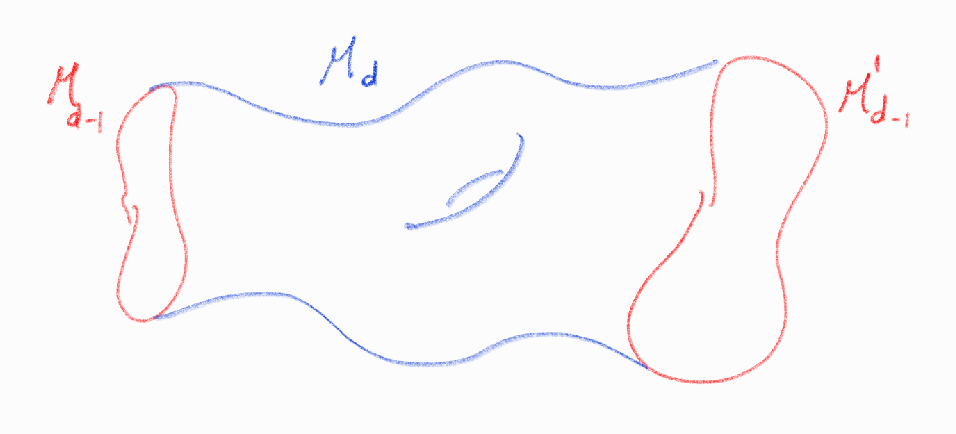
\includegraphics[width=0.75\linewidth]{images/1 Stokes theorem_260702_161207.pdf}
    \caption{Deformation of the topological surface using Stokes' theorem.}
    \label{fig:stokes_deform}
\end{figure}

\paragraph*{Parallelism with the traditional formulation:} It is useful to compare this with the standard textbook formulation of symmetries. Traditionally, one chooses $\mathcal{M}_{d-1}$ to be a constant time slice $\Sigma_t$, look at FIG. \ref{fig:time_slice}.\footnote{This choice assumes that the spacetime manifold factorizes globally as $\mathcal{M} = \mathbb{R} \times \Sigma$, which is not always possible (for example, on a sphere $\mathcal{S}^2$).} In that case, we integrate the charge density over all space, and the "topological" property simply means that the total charge is independent of time ($dQ/dt = 0$), meaning it is a conserved quantity under time evolution.

\begin{figure}
    \centering
    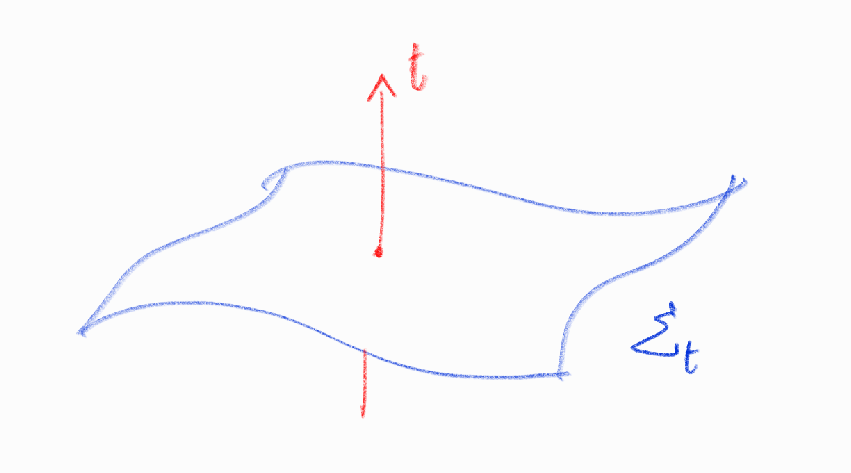
\includegraphics[width=0.75\linewidth]{images/2 Time slice _260702_161156.pdf}
    \caption{The traditional choice of integrating over a fixed time slice $\Sigma_t$.}
    \label{fig:time_slice}
\end{figure}

The charges $Q^a$ act as the generators of the Lie algebra $\frak{g}$. Using the exponential map from Lie theory, look at FIG. \ref{fig:exp_map}, we can construct the full symmetry operator associated with a finite group element $g \in G$:

\begin{equation}
U_g(\mathcal{M}_{d-1}) = \exp \left( i \alpha_a(g) Q^a(\mathcal{M}_{d-1}) \right)
\end{equation}
where $\alpha_a(g)$ are the coordinates of the group element. The factor of $i$ in the exponent ensures that $U_g$ is a unitary operator when the charges $Q^a$ are chosen to be Hermitian.

\begin{figure}
    \centering
    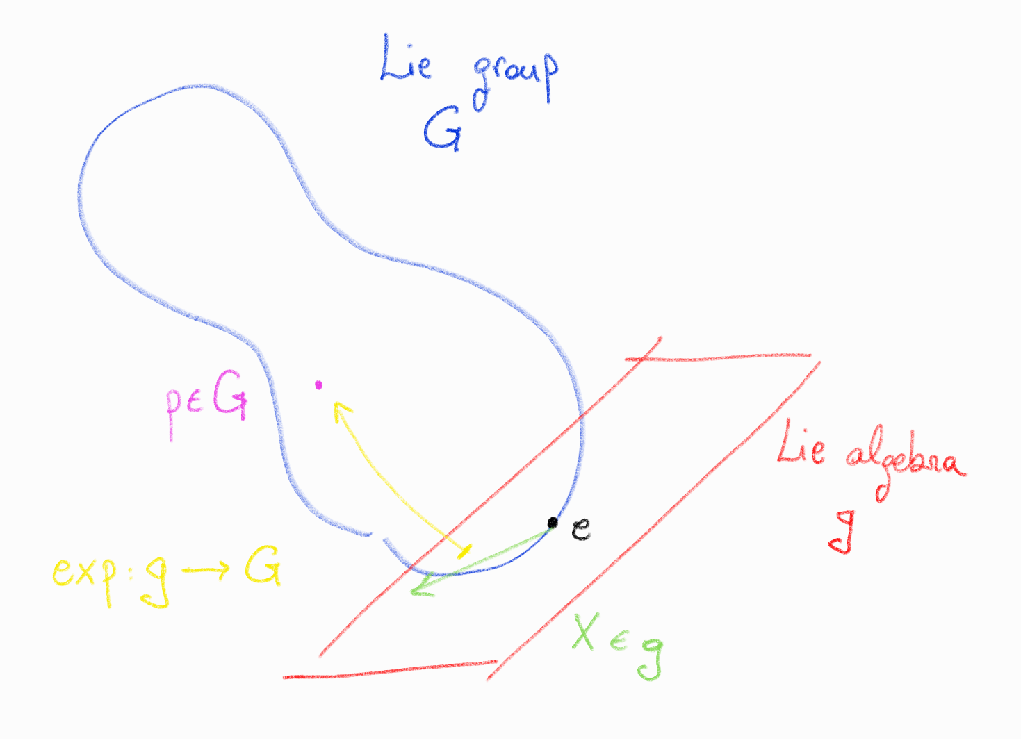
\includegraphics[width=0.75\linewidth]{images/3 exponential lie map_260702_161758.pdf}
    \caption{The exponential map sending elements from the Lie algebra to the Lie group.}
    \label{fig:exp_map}
\end{figure}

\paragraph*{Fusion rule property:} These symmetry operators satisfy a crucial property called the fusion rule. If we bring two parallel topological operators $U_g$ and $U_{g'}$ close to each other on the same surface, they fuse according to the group multiplication law:
\begin{equation}
    \lim_{\mathcal{M'}\to\mathcal{M}} U_{g'}(\mathcal{M'}) U_{g}(\mathcal{M}) = U_{g'g}(\mathcal{M})
\end{equation}
Note that this group structure does not need to be Abelian. 

An important property of any topological operator is that if we choose $\mathcal{M}_{d-1}$ to be a small sphere $\mathcal{S}^{d-1}$ enclosing a region with no other operator insertions, the sphere can be continuously shrunk down to a point and completely evaluated to the identity operator: $U_g(\mathcal{S}^{d-1}) = \mathbb{I}$, look at FIG. \ref{fig:sphere_collapse}.

\begin{figure}
    \centering
    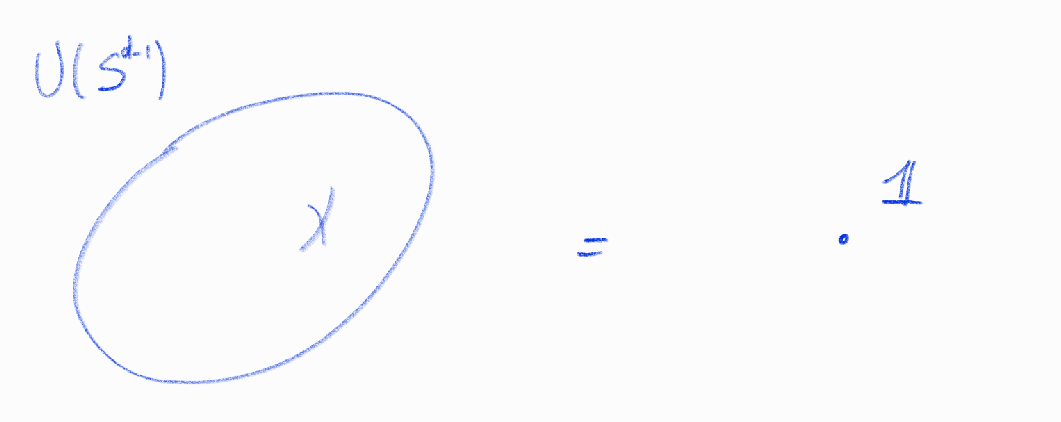
\includegraphics[width=0.75\linewidth]{images/4 sphere collapse_260702_162221.pdf}
    \caption{A topological sphere enclosing empty space collapses to the identity.}
    \label{fig:sphere_collapse}
\end{figure}

\subsubsection{Charged operators, representations and selection rules}\label{sec:charg-op_rep_sel-rule}

The local operators $\mathcal{O}(x)$ in our theory are classified by the representations of the symmetry group $G$. When a small topological sphere $U_g(\mathcal{S}^{d-1})$ encloses a local operator $\mathcal{O}_i(x)$ transforming in a representation $\rho$, shrinking the sphere down elements a linear transformation given by the representation matrix $\rho(g)_{ij}$:
\begin{equation}
    U_g (\mathcal{S}^{d-1}) \mathcal{O}_i (x) = \sum_j \rho(g)_{ij} \mathcal{O}_j(x)
\end{equation}
Look at FIG. \ref{fig:sphere_charged_op}.

\begin{figure}
    \centering
    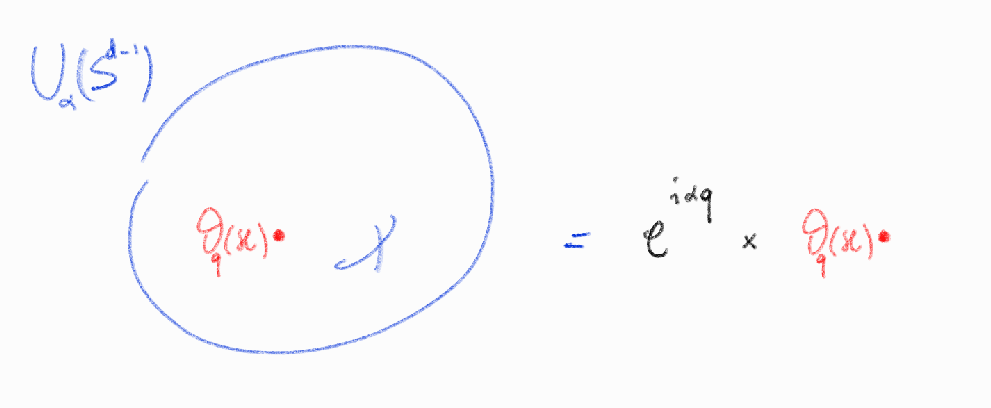
\includegraphics[width=0.75\linewidth]{images/5 sphere charge op_260702_163801.pdf}
    \caption{A topological sphere enclosing a charged operator is acting on it. As an example the group is $U(1)$ and the operator has charge $q$.}
    \label{fig:sphere_charged_op}
\end{figure}

This geometric picture allows us to easily derive selection rules and global Ward-Takahashi identities within correlation functions, look at FIG. \ref{fig:selection_rule}. Since a topological operator can be freely created from the identity, we can introduce a small sphere $U_g$ around empty space and then continuously deform it to wrap around the local operators inside the correlation function. As the surface crosses the operators, they transform under their respective representations. If the space is regularized or compactified, we can eventually push the defect to infinity where it evaluates back to the identity, yielding a powerful constraint on the correlator.

For example, consider a correlation function of three operators $\langle \mathcal{O}^A(x) \mathcal{O}^B(y) \mathcal{O}^C(z) \rangle$. By creating and expanding a topological defect, we find:
\begin{align}
    \langle \mathcal{O}^A_{\rho^A}(x) \mathcal{O}^B_{\rho^B}(y) \mathcal{O}^C_{\rho^C}(z) \rangle &= \langle U_g(\mathcal{S}^{d-1}) \mathcal{O}^A_{\rho^A}(x) \mathcal{O}^B_{\rho^B}(y) \mathcal{O}^C_{\rho^C}(z) \rangle \\
    &= \rho^A(g) \rho^B(g) \rho^C(g) \langle \mathcal{O}^A_{\rho^A}(x) \mathcal{O}^B_{\rho^B}(y) \mathcal{O}^C_{\rho^C}(z) \rangle
\end{align}
This equation implies that if the product of the representations does not contain the trivial singlet representation, the correlation function must vanish identically. For instance, in our complex scalar theory, a two-point function like $\langle \phi(x) \phi(y) \rangle$ is zero because the total $U(1)$ charge is not zero, meaning it cannot be invariant under the phase rotation.

\begin{figure}
    \centering
    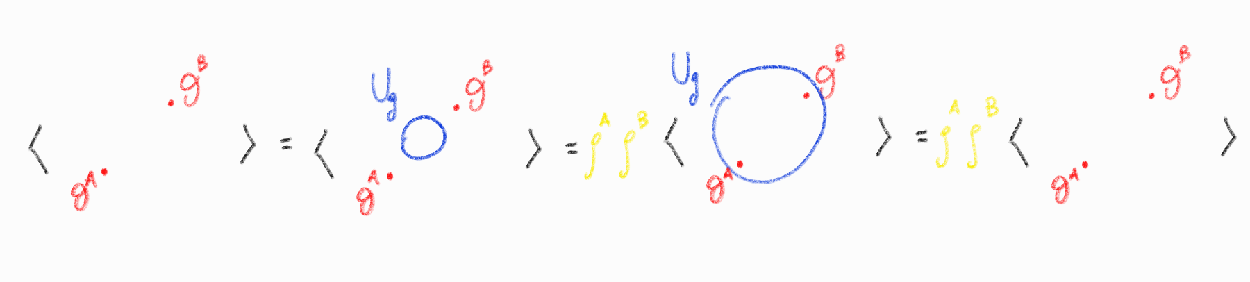
\includegraphics[width=1\linewidth]{images/6 section rules_260702_164446.pdf}
    \caption{Geometric derivation of a selection rule by deforming a topological operator through insertions.}
    \label{fig:selection_rule}
\end{figure}

\subsubsection{Summary \& Generalizations}

We have learned that an ordinary global symmetry can be fully encoded by its topological operators and how they fuse (which forms a group structure), while the charged objects are governed by the representations of that group.

\begin{tcolorbox}
{\bf Generalization Outlook}

This perspective opens the door to generalized symmetries. In the modern framework, the collection of topological defects forms a more general mathematical structure called a fusion category $\mathcal{C}$, and the charged objects are described by structures related to its modules or representations. This mathematical language extends far beyond standard group theory.
\end{tcolorbox}

Going back to our second question, generalized symmetries arise when we remove two main constraints from ordinary symmetries: the dimension of the topological operator is no longer restricted to be $d-1$, and the composition law is no longer required to follow a group structure.

The first generalization leads to \textbf{$p$-form symmetries}. If a theory contains a topological operator of dimension $d-p-1$, we say it possesses a $p$-form symmetry. The operators that carry a well-defined charge under a $p$-form symmetry are extended objects of dimension $p$ (such as lines, surfaces, etc.), loof at FIG. \ref{fig:p_form_link}.

\begin{figure}
    \centering
    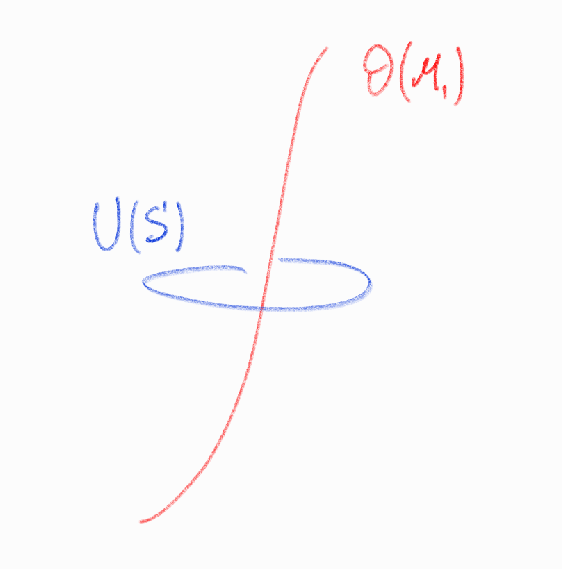
\includegraphics[width=0.5\linewidth]{images/7 higher form_260702_164609.pdf}
    \caption{A $(d-p-1)$-dimensional topological defect linking with a $p$-dimensional charged extended operator.}
    \label{fig:p_form_link}
\end{figure}

The second generalization leads to \textbf{non-invertible symmetries}. When two topological operators $U_a$ and $U_b$ fuse, the result does not have to be a single simple operator. Instead, it can decompose as a linear combination of different simple topological operators:
\begin{equation}
    \lim_{\mathcal{M'}\to\mathcal{M}} U_{a}(\mathcal{M'}) U_{b}(\mathcal{M}) = \sum_c \mathcal{N}^c_{ab} U_{c}(\mathcal{M})
    \label{eq:fusion_non_inv}
\end{equation}
where $\mathcal{N}^c_{ab}$ are non-negative integer coefficients. Because the right-hand side can be a sum of multiple distinct defects, an inverse operator does not generally exist. We will expand on the concept of simple operators and their fusion in section \ref{sec:simple_topo_op}.

\subsection{Interlude A: The Third Question: Local Symmetries?}\label{section:local_symmetry}

To clarify the conceptual confusion present in literature such as \cite{Barcel__2016}, a rigorous distinction between global and local transformations must be established based on the nature of the transformation parameters. Let a generic field transformation be denoted by $\mathcal{L}_\alpha[\phi] = \phi'$. A transformation is defined as \textit{global} if the parameter $\alpha$ is a spacetime constant. It constitutes a physical symmetry if it leaves the action invariant,\footnote{More accurately, the path integral measure composed by $\mathcal{D}\phi e^{-\mathcal{S}[\phi]}$.} thereby generating a non-trivial conserved Noether charge. Conversely, a transformation is \textit{local} if the parameter $\alpha(x)$ is an arbitrary function of spacetime coordinates. Local transformations correspond to gauge symmetries, which reflect a descriptive redundancy of the field variables rather than physical transformations; via Noether's second theorem, they yield off-shell identities where the current takes a superpotential form, rendering the associated physical charges identically zero on-shell.

Under this formal classification, the transformations designated as ``local'' in \cite{Barcel__2016} within Klein-Gordon theory—namely the transformation $\mathcal{L}_\alpha [\phi] = \phi + \alpha \chi$, where $\chi(x)$ is a fixed, specific solution to the Klein-Gordon equation $(\Box - m^2)\chi = 0$—are strictly \textit{global} symmetries. The dynamical parameter generating the transformation is the rigid constant $\alpha \in \mathbb{R}$, whereas the spacetime-dependent profile $\chi(x)$ is merely a fixed function. Because the true parameter $\alpha$ is a constant, the symmetry is \textit{global}. This structurally explains why it yields non-trivial, non-vanishing Noether charges and circumvents the first-class constraint framework typical of genuine gauge redundancies.

Furthermore, this algebraic property generalizes to any field theory governed by a linear differential operator $\hat{D}$. Whenever the classical equations of motion are linear ($\hat{D}\phi = 0$), the principle of linearity dictates that shifting a solution by another scaled classical solution $\alpha \chi$ generates a second solution. This framework yields an infinite-dimensional group of rigid symmetries parameterized by the solutions of the linear operator. Physically, this infinite set of conservation laws corresponds to the independent conservation of individual Fourier modes, reflecting the underlying linear dispersion relation. This precise symmetry structure provides the fundamental physical justification for employing the Fourier transform to diagonalize the differential operator within momentum space.

\subsection{Interlude B: Generalized Symmetries in Non-Relativistic Settings}\label{section:non_relativistic_symmetries}

So far, our exploration of generalized symmetries has relied heavily on the concept of \textit{topological} operators—defects that can be freely deformed in spacetime without changing correlation functions. However, if we relax the constraint of Lorentz invariance, entirely new families of generalized algebraic structures emerge, which are deeply rooted in condensed matter physics and non-relativistic field theories \cite{cordova2022snowmasswhitepapergeneralized, McGreevy_2023}.

The first major class consists of \textbf{subsystem symmetries}. While higher-form symmetries feature charges that depend strictly on the topology of the support manifold, subsystem symmetry operators act on rigid, fixed subspaces of space, such as lines, planes, or even fractals. Because these operators are sensitive to the exact geometry, shape, and location of the subspace rather than just its topology, they drastically constrain the dynamics of the system. This framework provides the underlying symmetry structure for \textbf{fracton phases}, where the charged excitations exhibit restricted mobility and are locked to specific spatial loci.

A parallel generalization is found in \textbf{multipole symmetries}, where the standard continuity equation is modified by higher spatial derivatives. A classic example is a dipole symmetry satisfying $\partial_0 J^0 + \partial_i \partial_j J^{ij} = 0$, which requires the conservation of both total charge and total dipole moment. This conservation law physically prevents individual isolated charges from moving, allowing only neutral bound states to be mobile. 

At low energies, systems with subsystem and multipole constraints cannot be captured by conventional vector gauge fields. Instead, they require exotic \textbf{higher-rank tensor gauge theories}. Mathematically, these theories share a common algebraic language with the gauge structures of linearized gravity and its modern formulation via relativistic \textbf{biform symmetries} \cite{Hinterbichler_2023}, as both frameworks generalize ordinary $p$-forms to higher-rank tensor representations. However, a crucial distinction must be made: while biform symmetries protect the masslessness of the graviton in a fully Lorentz-invariant setup, the non-relativistic nature of fractonic theories leads to a severe form of UV/IR mixing, making the long-distance low-energy physics explicitly sensitive to short-distance lattice details and geometric properties, breaking the EFT paradigm.


\subsection{Higher $p$-form symmetries} \label{sec:p-form_sym}

In the following we explain in more detail the first generalization we have already mentioned, namely the dimensionality of the topological operators is not anymore constrained to be $d-1$, look at FIG. \ref{fig:p_form_link}. 

  \subsubsection{$p$-form symmetries and $d-p-1$-dimensional defects}
Baptizing these new symmetries: $p$-form symmetries, we now explain what this $p$ stands for, which as an anticipation is the dimension of the smallest possible charged operator. Using this nomenclature, the ordinary symmetries are called $0$-form symmetries, where the smallest possible charged operators are $0$-dimensional, i.e. local operators.
\begin{equation}
    \text{Ordinary Symmetry} = \text{$0$-form Symmetry}
\end{equation}

In this case, the symmetry operator (the topological operator) is $(d-p-1)$-dimensional, i.e. $U(\mathcal{M}_{d-p-1})$. Notice that in this situation we cannot anymore take advantage of the double interpretation: topological operator in the Euclidean setting and Quantum mechanical operator acting on the Hilbert space at a given time. We cannot pick $\mathcal{M}_{d-p-1} = \Sigma_t$.
\begin{equation}
    \text{$p$-form Symmetry} \iff \text{$(d-p-1)$-dimensional Topological Operator}
\end{equation}


Similarly with the ordinary group symmetries, when our symmetry is continuous we have an expression for a local current, which instead of being a closed $d-1$-closed differential form, it is a $d-p-1$-closed differential form.\footnote{Actually, instances of non-invertible continuous symmetries that have a topological symmetry operator have been found, but not an expression for a local current.}

\begin{equation}
    \text{Continuous $p$-form $G$-Symmetry} \iff \text{Closed } \frak{g}\text{-valued } (d-p-1)\text{-form}
\end{equation}

\begin{tcolorbox}[colback=green!5!white, colframe=green!75!black, title={Example: $1$-form symmetry from Superfluid}]
One of the simplest example is the free scalar boson in $3$d. 

\begin{equation}\label{eq:superfluid}
    \mathcal{S} = \int_{\mathcal{M}_3} d \phi \wedge \star d \phi
\end{equation}

We have already mentioned the $0$-form symmetry, whose current is $\star j^{(1)}_A = \star d \phi$, and the closedness is guaranteed by the EOM. What we have not mentioned yet is another closed form that the theory has, namely $\star j^{(2)}_B = d \phi$, whose closedness is enforced by how we decided to describe the theory: $d\star j^{(2)}_B = dd\phi = 0 $.

In this example, the symmetry operators are: 

\begin{equation}\label{eq:1form_sym-op}
    U^A_\alpha (\mathcal{M}_{2}) = \exp \{ i \alpha \int_{\mathcal{M}_{2}} \star j^{(1)}_A \} \qquad \& \qquad U^B_\beta (\mathcal{M}_{1}) = \exp \{ i \beta \int_{\mathcal{M}_{1}} \star j^{(2)}_B \}
\end{equation}

\end{tcolorbox} 

Before moving on, there is an insightful thing we can point out at this point: a duality. In fact, the example we have just presented has a dual counter part: the Free Maxwell Theory in $3$d.\footnote{The modern understanding of a duality is the following: the two theories are the same theory, what makes them different in appearance is simply the choice of fundamental degrees of freedom used to describe it. As in a vector space we have freedom to choose a basis (also called a frame), in a QFT we have freedom to choose what to call "fundamental degree of freedom", which is simply the integration variable of the path integral; using this analogy, the two dual theories are called duality frames.}

\begin{tcolorbox}
    {\bf The Particle-Vortex Duality}

    Since it is quite straightforward, let us present the derivation of the duality.
    
\begin{align}
    \mathcal{Z} &= \int \mathcal{D}\phi^{(0)} \exp \left( -\int d \phi^{(0)} \wedge \star d \phi^{(0)} \right) \\
    &= \int \mathcal{D}v^{(1)} \mathcal{D}a^{(d-2)} \exp \left( -\int v^{(1)} \wedge \star v^{(1)} + 2ia^{(d-2)} \wedge dv^{(1)} \right) \\
    &= \int [...] \exp \left( -\int (v^{(1)}- i\star da^{(d-2)}) \wedge \star (v^{(1)}- i\star da^{(d-2)}) + da^{(d-2)} \wedge \star da^{(d-2)} \right) \\
    &= \# \int \mathcal{D}a^{(d-2)} \exp \left( -\int  da^{(d-2)} \wedge \star da^{(d-2)} \right) \\
\end{align}

Where from the first to the second line we used the substitution $d\phi^{(0)} = v^{(1)}$, but since we should not integrate over all $d$ local degrees of freedom of a generic $1$-form, we enforce it to be closed using a Lagrange multiplier: $a^{(d-2)}$, which is a $(d-2)$-form.\footnote{Counting DOF is instructive, recall that for a higher $p$-gauge field, the number of DOF is equal to $\frac{(d-2)}{p}$, which is given by the dimension of the transverse representation. Regarding $\phi^{(0)}$, $p=0$ and then we have one DOF; regarding $a^{(d-2)}$, being a $d-2$-form we again have one DOF.} In the third line we simply "completed the square", and in the last line we integrated out $v^{(1)}$, since it compared in a Gaussian form, and then the integral is exactly solvable.

What happened, is that we packaged the information in $\mathcal{Z}$ in two different ways, the first is a free scalar boson theory and the second is a generalized Maxwell theory.\footnote{We should think of $a^{(d-2)}$ as the local representation of the connection of the gauge theory, what we usually call $A$, while what we integrate at the end is the curvature, what we usually call $F$, and as it should be it is gauge invariant.} Even more explicitly, in the $\phi^{(0)}$ duality frame, we make explicit the complex-magnitude excitations, while in the $a^{(d-2)}$ duality frame we make explicit the phase-winding excitations. From the point of view of the Hilbert space, there is no hierarchy between these two different excitations.\footnote{We might think of this as a drawback of using the Lagrangian formalism. It forces us to reason semiclassically (if the theory is not free or solvable).}

If we restrict ourself to $3$-dimensions, $a^{(d-2)}$ is a $1$-form and then we obtain ordinary Maxwell theory (Electromagnetism), but in $3$ spacetime dimensions.
    
\end{tcolorbox}

Since we have just learned that the same theory can be presented in (at least) two different ways, we could present the $1$-form example using both microscopical descriptions. The first one, we already did; the second one, we present it now.

\begin{tcolorbox}
    {\bf Same example, but different duality frame}
    
\begin{align}
    \mathcal{Z} = \# \int \mathcal{D}a^{(d-2)} \exp \left( -\int  da^{(d-2)} \wedge \star da^{(d-2)} \right) \\
\end{align}


Since the two theories are the same theory, we must be able to indentify the symmetries in the new duality frame. In fact, $\star j^{(1)}_A=da^{(d-2)}$ and $\star j^{(2)}_B=\star da^{(d-2)}$; furthermore, notice that the reason why these differential forms are closed is different, has switched, from the other duality frame: $d\star j^{(1)}_A=dda^{(d-2)}=0$ just thanks to the formalism, while $d\star j^{(2)}_B=d\star da^{(d-2)}$ is equal to zero only when evaluated on the EOM.

The symmetry operators are, unsurprisingly, exactly what we have already wrote in \ref{eq:1form_sym-op}.

    
\end{tcolorbox}
  
  \subsubsection{Charged objects and higher-form charges}
  
Having genreralized the dimension of the topological operators that represent symmetries, it is time to consider what objects are charged under these symmetry operators.

\paragraph*{The problem:} in the case of a $1$-form symmetry let us say in $3d$ for concreteness, the associated topological operator is $1$-dimensional, i.e. a line (let us pick a closed circle line for concreteness). We immediately realize that a local operator cannot be charged WRT this symmetry: in $3d$, a line cannot surround a point. Since the line is topological, it is free to move as long as it does not pass through anything; if around space we have only point-local operators, the circle can always be contracted to a point, i.e. the identity operator.\footnote{Actually, after the contraction, we in principle obtain a local topological operator, but we prefer to treat them separately and restrict ourself to the case of it being the identity operator. To know a little more about local topological operators, look at \ref{sec:topo_loc_op}.}

Then we conclude that for the case of a $1$-form symmetry, the smallest charged object has to be of dimension $1$. This is easily generalizable: the smallest charged object WRT a $p$-form symmetry is $p$-dimensional.\footnote{You can also think in the following way: two $p$-dimensional extended objects in $d$-dimensions, if $p < d-1$ the objects have room to move around each others, while if $p=d-1$ they have to link to pass each others.}

Again, exactly in the same way of ordinary group symmetries, when the symmetry is group like the charged objects are labelled by the representations of the symmetry group.

\begin{equation}
U_g (\mathcal{S}^{d-p-1}) \mathcal{O}_\rho (\mathcal{M}_p) =  \rho_g [\mathcal{O}(\mathcal{M}_p)]
\end{equation}
 



For abelian higher-form symmetries, this representation reduces to a simple phase factor. When the codimension-$(p+1)$ topological symmetry operator $U_g(\mathcal{S}^{d-p-1})$ links with a $p$-dimensional defect $\mathcal{O}(\mathcal{M}_p)$, the intersection yields:\begin{equation}U_g (\mathcal{S}^{d-p-1}) \mathcal{O}(\mathcal{M}_p) = e^{i q \cdot g} \mathcal{O}(\mathcal{M}_p)\end{equation}where $q$ denotes the charge of the defect. We define generalized charges carried by $p$-dimensional operators as \textbf{$p$-charges}. 

\begin{tcolorbox}[colback=green!5!white, colframe=green!75!black, title={Example: Wilson lines and Representations}]
Consider a $U(1)$ gauge theory. A Wilson line operator $W_\rho(\mathcal{C})$ supported on a closed loop $\mathcal{C}$ is defined by choosing an irreducible representation $\rho$ of the gauge group, which is labeled by an integer charge $q$:
\begin{equation}
    W_\rho(\mathcal{C}) = \exp \left( i q \oint_{\mathcal{C}} A \right)
\end{equation}
The global $1$-form symmetry of this theory is $U(1)$. When a codimension-$2$ topological symmetry operator links with the loop $\mathcal{C}$, it acts on the gauge connection by a group transformation $\alpha \in U(1)$. 

Under this action, the Wilson line transforms directly via the representation $\rho$:
\begin{equation}
    W_\rho(\mathcal{C}) \longrightarrow \rho(\alpha) W_\rho(\mathcal{C}) = e^{i q \alpha} W_\rho(\mathcal{C})
\end{equation}
This explicit phase factor shows that the choice of the representation $\rho$ physically dictates the $1$-form charge of the line operator.
\end{tcolorbox}

Crucially, the standard paradigm stating that a $p$-form symmetry only acts on $p$-dimensional objects is incomplete. A $p$-form symmetry can also constrain $q$-dimensional operators ($q$-charges) where $q \neq p$. The general underlying algebraic principle is that the $q$-charges of a $p$-form symmetry $G^{(p)}$ are classified by \textbf{$(q+1)$-representations} of the symmetry group \cite{schafernameki2023ictplecturesnoninvertiblegeneralized}. 

To illustrate this, consider a $0$-form global symmetry group $G^{(0)}$ acting on a $1$-dimensional line operator $\mathcal{O}_1$ (a $1$-charge). The $0$-form symmetry generator $D_g$ maps the line to a potentially distinct line $g\mathcal{O}_1$, organizing the operators into orbits. The subgroup of $G^{(0)}$ that leaves a given line operator invariant is its stabilizer group $H \subset G^{(0)}$. At the junction where the symmetry generators intersect the line, they induce a lower-dimensional topological symmetry localized strictly on the defect. The fusion of these induced operators $D_0(h)$ on the line can be projective, meaning it is modified by a 't Hooft anomaly phase specified by a 2-cocycle $\sigma \in H^2(H, U(1))$:\begin{equation}D_0(h_1) \otimes D_0(h_2) = \sigma(h_1, h_2) D_0(h_1 h_2)\end{equation}The pair $(H, \sigma)$ uniquely characterizes a 2-representation of $G^{(0)}$.

\begin{tcolorbox}[colback=green!5!white, colframe=green!75!black, title={Example: Free Maxwell in $4d$}]
    A standard example is a $4d$ $U(1)$ gauge theory under a $\mathbb{Z}_2^{(0)}$ charge conjugation symmetry ($A \to -A$), also called Outer Automorphism. This $0$-form symmetry acts on the $1$-dimensional Wilson lines by mapping $W_\alpha \to W_{-\alpha}$. For a generic charge $\alpha$, the lines $W_\alpha$ and $W_{-\alpha}$ form a 2-dimensional orbit with a trivial stabilizer $H = 1$, corresponding to the regular 2-representation. Conversely, for the discrete charges $\alpha = 0, \pi$, the lines are invariant under charge conjugation; their stabilizer is the full group $H = \mathbb{Z}_2$, which realizes the non-trivial 2-representation.
\end{tcolorbox}


This framework generalizes to arbitrary dimensions: the $q$-charges of a $p$-form symmetry group correspond to $(q+1)$-representations $\rho^{(q+1)}$, which are determined by the stabilizer subgroups $H$ of the operator orbits and the corresponding higher cohomology groups $H^{q+1}(H, U(1))$.
  
  \subsubsection{Fusion rules and higher-form selection rules}
This paragraph generalizes straightforwardly the discussion over ordinary symmetries. 

\paragraph*{Fusion rules:} The only difference we have here WRT ordinary symmetries, i.e. fusing $d-1$-dimensional topological operators, is that we are fusing $d-p-1$-dimensional operators, loof at FIG. \ref{fig:highform_fusion}.

\begin{equation}
\lim_{\mathcal{M'} \to\mathcal{M} } U_{g'}(\mathcal{M'}_{d-p-1})U_{g}(\mathcal{M}_{d-p-1}) = U_{g' g}(\mathcal{M}_{d-p-1})
\end{equation}

This dimension generalization carries even a further semplification: the fusion rules have to be Abelian (i.e. commutative). This can be understood in $3d$ for concreteness by picking two $1d$ topological operators; for two $1d$ objects in $3d$ there is no notion of order, opposed to $2d$ objects (i.e. ordinary symmetries). This means that ordinary symmetries need Non-Abelian groups to be described in general, while higher-form symmetries (when group-like) only need Abelian groups.\footnote{Non-invertible symmetries will need a structure beyond the one of a group, but when higher forms they will still have the Abelian property.}

\begin{figure}
    \centering
    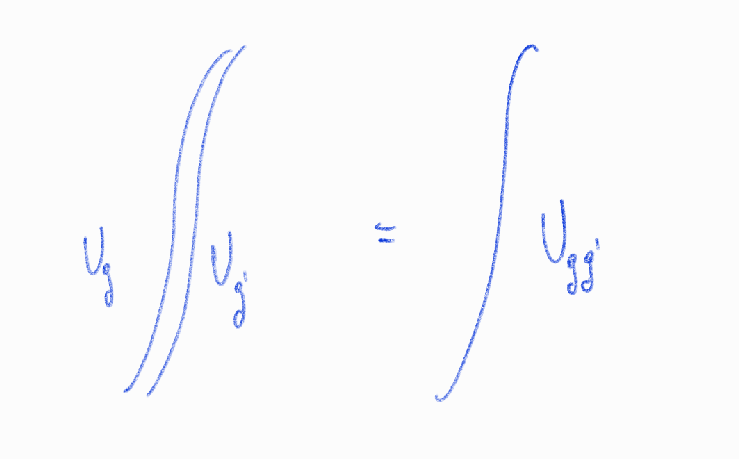
\includegraphics[width=0.65\linewidth]{images/9 fusion 1form_260702_165347.pdf}
    \caption{The Fusion of $1$-form group-like topological operators in $3d$.}
    \label{fig:highform_fusion}
\end{figure}

\paragraph*{Selection rules:} Analogously, we have (Global) Ward-Takahashi identities which lead to selection rules, exactly as in \ref{sec:charg-op_rep_sel-rule}. Look at FIG. \ref{fig:higher_selection_rules}. So given as an example the correlation function of three extended operators charged WRT a $p$-form symmetry:

\begin{align}
    \mathcal{O}^A_{\rho^A} (\mathcal{M}_p) \mathcal{O}^B_{\rho^B} (\mathcal{N}_p) \mathcal{O}^C_{\rho^C} (\mathcal{X}_p) 
    &= U_g (\mathcal{S}_1^{d-p-1}) \mathcal{O}^A_{\rho^A} (\mathcal{M}_p) \mathcal{O}^B_{\rho^B} (\mathcal{N}_p) \mathcal{O}^C_{\rho^C} (\mathcal{X}_p) \\
    &= U_g (\mathcal{S}_2^{d-p-1}) \rho^A_g [\mathcal{O}^A(\mathcal{M}_p)] \mathcal{O}^B_{\rho^B} (\mathcal{N}_p) \mathcal{O}^C_{\rho^C} (\mathcal{X}_p) \\
    &= \rho^A_g [\mathcal{O}^A(\mathcal{M}_p)] \rho^B_g [\mathcal{O}^B(\mathcal{N}_p)] \rho^C_g [\mathcal{O}^C(\mathcal{X}_p)]
\end{align}

The theory possessing the symmetry is thus constrained to satisfy the above identity. 
Consequently, in the unbroken phase, a correlation function of charged extended operators is non-vanishing if and only if the total fused charge of the configuration is trivial under the action of $G^{(p)}$. For abelian symmetries, this translates to the strict conservation law $\sum_{i} q_i = 0$.

\begin{figure}
    \centering
    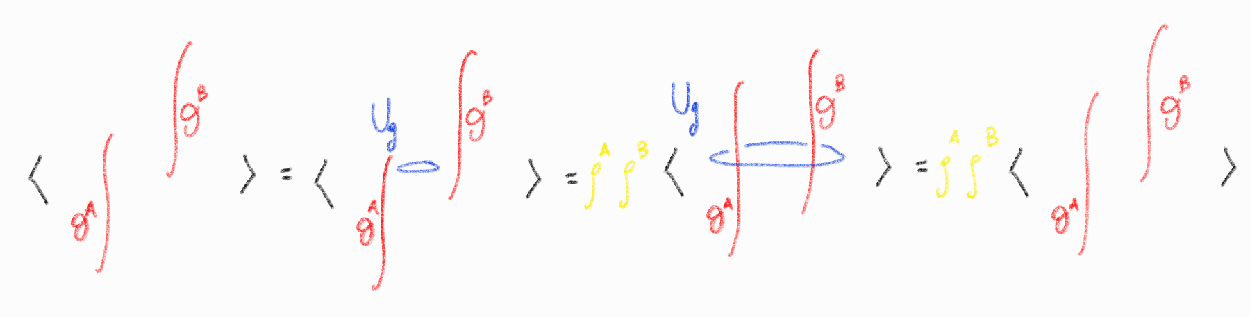
\includegraphics[width=1\linewidth]{images/10 section rules highform_260702_165544.pdf}
    \caption{Selection rule for $1$-form symmetries in $3d$.}
    \label{fig:higher_selection_rules}
\end{figure}


\subsubsection{Gauging a symmetry and the Dual Symmetry}
\label{sec:gauging_and_dual}

    
    As for ordinary symmetries, higher form symmertries can be coupled to group-valued (when discrete, algebra-valued when continuous) background fields.\footnote{Since we have not discussed the case of non-invertible symmetries yet, we are assuming the discussion over higher form symmetries regards group-like structures, even though higher-form symmetries can of course be non-invertible.}  

  \begin{tcolorbox}
      {\bf Background fields for Ordinary Symmetries}

      A background field $B$ for a $0$-form symmetry with group $G^{(0)}$ is a specification of holonomies $g_{\mathcal{M}_1} \in G^{(0)}$ for every closed $1$-cycle $\mathcal{M}_1$ in the following sense
      \begin{equation}
        g_{\mathcal{M}_1} = \exp \left( i \oint_{\mathcal{M}_1} B \right)
      \end{equation}
      with two requirements for the holonomy: 
      
      \begin{enumerate}[\itshape i)]
          \item being the identity element if the $1$-cycle is contractible, which translates to the closure condition $dB=0$.

          \item being invariant under gauge transformations $B \to B + d\Lambda$.
      \end{enumerate}
      Formally, this means $B \in H^1(\mathcal{M}, G^{(0)})$ \cite{schafernameki2023ictplecturesnoninvertiblegeneralized}.\footnote{This is the cohomology WRT the smooth manifold differential operator (de Rham differential) and Lie algebra-valued 1-forms (when discussing continuous groups, for discrete ones its is group-valued).}
  \end{tcolorbox}

  The higher-form generalization is straightforward. A background field $B^{(p+1)}$ for a $p$-form symmetry with group $G^{(p)}$ is a specification of holonomies $g_{\mathcal{M}_{p+1}}$ for every closed $\mathcal{M}_{p+1}$.\footnote{Throughout this thesis we will refer to the attribute closed according with the physics community, which uses it meaning without boundaries, and not in the mathematical sense: the complementary be open (according to the topology chosen).}
  \begin{equation}
    g_{\mathcal{M}_{p+1}} = \exp \left( i \oint_{\mathcal{M}_{p+1}} B^{(p+1)} \right)
\end{equation}
with the same two requirements, then $B^{(p+1)} \in H^{p+1}(\mathcal{M}, G^{(p)})$.

\paragraph*{The Dual Symmetry of Flat Gauging:} 
A $p$-form symmetry $G^{(p)}$ inherently implies a dual $(d-p-2)$-form symmetry governed by the Pontryagin dual group $\hat{G}^{(d-p-2)}$. This specific duality mapping is realized strictly via flat gauging. For continuous symmetries, the gauging procedure bifurcates into flat and dynamical implementations; this topological framework governs exclusively the flat sector. Conversely, for finite discrete symmetries, flat gauging constitutes the unique choice, requiring an explicit summation over all flat background field configurations.\footnote{The attributes flat and non-flat distinguish whether the path integral restricts configurations to vanishing curvature or integrates over generic, non-vanishing field strengths. This means that flat gauging is just summing over flat bundles.} This operation is called to be topological in the sense that it does not affect the local structure of the theory, it does commute with the RG flow.

\begin{align}
    \left\{ \begin{matrix} 
    (p)\text{-form symmetry} \\ 
    B^{(p+1)} \in H^{p+1}(\mathcal{M}_d,G^{(p)})
    \end{matrix} \right\} 
 \xleftrightarrow{\text{\quad flat gauging \quad}}
\left\{ \begin{matrix} 
    (d-p-2)\text{-form symmetry} \\ 
    \hat{B}^{(d-p-1)} \in H^{d-p-1}(\mathcal{M}_d,\hat G^{(d-p-2)})
    \end{matrix} \right\} 
\end{align}

For a finite Abelian $p$-form symmetry group $G^{(p)}$, gauging proceeds by summing over all flat background configurations, acting as a generalized discrete Fourier transform on the partition function space. Let $\mathcal{Z}_T[B^{(p+1)}]$ denote the partition function of the theory $\mathcal{T}$ coupled to the background $B^{(p+1)} \in H^{p+1}(\mathcal{M}_d, G^{(p)})$. The partition function of the gauged theory $\mathcal{T} / G^{(p)}$ in the presence of a dual background field $\hat{B}^{(d-p-1)}$ is defined by the topological sum:
\begin{equation}
\mathcal{Z}_{\mathcal{T}/G^{(p)}}[\hat{B}^{(d-p-1)}] = \frac{1}{\sqrt{|H^{p+1}(\mathcal{M}_d, G^{(p)})|}} \sum_{B^{(p+1)} \in H^{p+1}(\mathcal{M}_d, G^{(p)})} e^{2\pi i \langle B^{(p+1)}, \hat{B}^{(d-p-1)} \rangle} \mathcal{Z}_\mathcal{T}[B^{(p+1)}].
\end{equation}
The phase factor dictates the topological coupling between the original and dual background fields. The bilinear pairing
\begin{equation}
\langle \cdot, \cdot \rangle: H^{p+1}(\mathcal{M}_d, G^{(p)}) \times H^{d-p-1}(\mathcal{M}_d, \hat{G}^{(d-p-2)}) \longrightarrow \mathbb{R}/\mathbb{Z}
\end{equation}
is evaluated by leveraging Poincaré duality to map cohomology classes to intersecting cycles, combined with the canonical evaluation of the Pontryagin dual group:
\begin{equation}
\hat{G}^{(d-p-2)} \equiv \text{Hom}(G^{(p)}, U(1)).
\end{equation}
Dynamically, this dual architecture provides an explicit geometric construction for the topological defect operators that generate the symmetry. In the gauged theory $\mathcal{T}/G^{(p)}$, the dual background fields define the topological symmetry operators $\mathcal{D}_{d-p-1}$ supported on $(d-p-1)$-dimensional submanifolds via:
\begin{equation}
\mathcal{D}_{d-p-1}(\mathcal{M}_{d-p-1}) = \exp \left( i \oint_{\mathcal{M}_{d-p-1}} \hat{B}^{(d-p-1)} \right).
\end{equation}
These operators act non-trivially on the $p$-dimensional defects $\mathcal{O}_p$ of the original theory. Symmetrically, the original background fields $B^{(p+1)}$, stripped of their classical background interpretation by the path integral summation, define the dual defect operators $\hat{\mathcal{D}}_{p+1}$ supported on $(p+1)$-dimensional submanifolds:
\begin{equation}
\hat{\mathcal{D}}_{p+1}(\mathcal{M}_{p+1}) = \exp \left( i \oint_{\mathcal{M}_{p+1}} B^{(p+1)} \right),
\end{equation}
which measure the topological charges of the dual $(d-p-2)$-dimensional defects. This bidirectional mapping ensures that a sequential second gauging returns the system to its initial un-gauged formulation, establishing an exact duality between the spectral data of both representations.

\paragraph*{The Dual Symmetry of Dynamical Gauging:} 
For continuous compact groups, such as $G^{(p)} = U(1)$, dynamical gauging promotes the background field $B^{(p+1)}$ to a dynamical connection $a^{(p+1)}$ by introducing a kinetic generalized Maxwell term $\frac{1}{2g^2}\int da\wedge \star da$ and integrating over its gauge equivalence classes.\footnote{Notice that this procedure introduce new DOF.}

At the level of currents, the original $p$-form symmetry was governed by a closed $(d-p-1)$-form current $\star j^{(p+1)}$, satisfying $d\star j^{(p+1)} = 0$. 
Gauging transforms this conservation law into a trivial topological identity: the current is rendered exact,\footnote{This trivialization is critical for $(-1)$-form symmetries. While the conservation condition is vacuous because every $d$-form is trivially closed, exactness remains non-trivial \cite{Heidenreich_2021}.} $\star j^{(p+1)} = d\omega^{(d-p-2)}$, matching the equation of motion of the newly dynamical field. The dual $(d-p-3)$-form symmetry emerges directly from the geometric conservation of the field strength, yielding the dual current $\star j^{(d-p-2)}_{\text{dual}} \sim da^{(p+1)}$.

\begin{align}
    \left\{ \begin{matrix} 
    (p)\text{-form symmetry} \\ 
    j^{(p+1)}, U_g(\mathcal{M}_{d-p-1})
    \end{matrix} \right\} 
 \xleftrightarrow{\text{\quad dynamical gauging \quad}}
\left\{ \begin{matrix} 
    (d-p-3)\text{-form symmetry} \\ 
    j^{(d-p-2)}, U_g(\mathcal{M}_{p+2})
    \end{matrix} \right\} 
\end{align}

Notice the double arrow, in fact, gauging again we come back to the initial theory.

\begin{tcolorbox}[colback=green!5!white, colframe=green!75!black, title={Example: Complex Scalar Boson $\xrightarrow{\text{\quad dynamical gauging \quad}}$ Scalar QED}]
        Consider the action of a complex scalar field coupled to a background $1$-form gauge field $B^{(1)}$:
    \begin{equation}
        \mathcal{S}[\phi; B^{(1)}, V] = \int \frac{1}{2}(d - iB^{(1)})\phi \wedge \star (d + iB^{(1)}) \bar \phi + V(|\phi|) \star 1
    \end{equation}
    The action is invariant under the global phase rotation $U(1)^{(0)}$, generating the conserved $1$-form current $\star j^{(1)} = i(\phi \star d \bar \phi - \bar \phi \star d \phi)$.

    Dynamical gauging promotes $B^{(1)}$ to a fluctuating connection $a^{(1)}$ by appending a kinetic term and integrating over the field space:
    \begin{equation}
        \mathcal{S}[\phi, a^{(1)};V, g] = \int \frac{1}{2}(d - ia^{(1)})\phi \wedge \star (d + ia^{(1)}) \bar \phi + V(|\phi|) \star 1 + \frac{1}{2 g^2} da^{(1)} \wedge \star da^{(1)}
    \end{equation}
    The original $U(1)^{(0)}$ symmetry is explicitly broken by the dynamics, giving rise to its dual $(d-3)$-form symmetry under dynamical gauging, whose current is explicitly defined as $\star j^{(d-2)}_{\text{dual}} \sim da^{(1)}$ and closed by the Bianchi identity.

    If we now gauge the $U(1)^{(d-3)}$ symmetry dynamically, adding the couplings $\int da \wedge b^{(d-2)} + \frac{1}{2 h^2}db\wedge \star db$, we obtain again the initial theory with symmetry $U(1)^{(0)}$ restored by $\star j^{(1)} \sim db^{(d-2)}$.
\end{tcolorbox}

As an example, given a symmetry $U(1)^{(p)}$, its flat gauging gives a dual symmetry $\mathbb{Z}^{(d-p-2)}$, while its dynamical gauging gives a dual symmetry $U(1)^{(d-p-3)}$.

\subsection{Interlude C: Gauging on Manifolds with Boundaries}\label{section:gauging_boundaries}

Dynamical gauging of a global symmetry group $G$ inherently trivializes bulk Noether charges, converting physical global symmetries into local gauge redundancies whose currents become exact forms on-shell. However, formulating the resulting gauge theory on a manifold $\mathcal{M}$ with a physical boundary or an asymptotic infinity $\partial \mathcal{M}$ fundamentally alters this paradigm. Variational consistency and the definition of a well-posed action require prescribing strict boundary conditions for both the gauge connections and the localized gauge parameters $\alpha(x)$. 

Gauge transformations that vanish or fall off sufficiently fast at the boundary constitute the \textit{proper} gauge redundancies, parameterizing unphysical, unobservable degrees of freedom. Conversely, gauge transformations that remain non-trivial or approach a rigid profile at $\partial \mathcal{M}$ are classified as \textit{improper} gauge transformations. These sustain a genuine physical status, operating as global symmetries localized strictly on the boundary. Consequently, the global symmetry dynamically eliminated in the bulk is resurrected on the geometric boundary of the theory.

Standard Maxwell electrodynamics offers a classic realization of this recovery mechanism. In the bulk, the local $U(1)$ phase rotation is a redundancy, and the field equations $d \star F = \star j$ identify the matter current with a total derivative. On a manifold with a boundary, however, the subgroup of gauge transformations stabilizing to a constant value at $\partial \mathcal{M}$ generates a non-trivial boundary global symmetry. The total electric charge $Q$ survives as a well-defined physical observable, mapped via Gauss's law to an integral over a codimension-2 boundary surface $\partial\Sigma$:
\begin{equation}
Q = \int_{\partial \Sigma} \star F
\end{equation}
where $\Sigma$ represents a spatial Cauchy slice and $\partial\Sigma \subset \partial\mathcal{M}$. 

This structure directly parallels general relativity: while bulk diffeomorphism invariance constitutes a local redundancy, asymptotic boundary conditions restrict the allowed coordinate transformations at infinity. The surviving transformations match the asymptotic Killing vectors of the background, yielding physical conserved surface charges such as the ADM energy and momentum. Ultimately, while these structures frequently appear under the heading of asymptotic symmetries, their physical nature is encoded in the structural presence of a boundary rather than the specific choice of an asymptotic infinite limit.

\subsection{Non-invertible generalized symmetries} \label{sec:non-inv_sym}

The second, more profound generalization relaxes the algebraic structure governing the fusion of topological operators: the traditional restriction to group-like compositions is abandoned in favor of a more comprehensive algebraic framework.

\subsubsection{From group-like fusion to categorical fusion}

In invertible or higher-form symmetries, the parallel collision of topological operators satisfies group-like fusion laws: $\lim_{\mathcal{M'} \to \mathcal{M}} U_{g'}(\mathcal{M}') U_g(\mathcal{M}) = U_{g'g}(\mathcal{M})$. The categorical paradigm generalizes this by requiring only that the parallel composition of two topological operators yields an operator that remains strictly topological. Consequently, the fusion closure can yield a linear combination of all admissible topological defects in the theory, formalized mathematically via a higher fusion category.

The formal justification for the existence of a vector space structure permitting these linear combinations is deferred to \ref{sec:topo_operator_space}. The generalized fusion rule for non-invertible symmetry defects reads:
\begin{equation}
\lim_{\mathcal{M'} \to\mathcal{M} } U_{a}(\mathcal{M'}_{d-p-1})U_{b}(\mathcal{M}_{d-p-1}) = \sum_c \mathcal{Z}^c_{ab} U_{c}(\mathcal{M}_{d-p-1})
\end{equation}
where the fusion coefficients $\mathcal{Z}^c_{ab}$ can encode topological partition functions of lower-dimensional internal TQFTs. Commutativity (the higher-form Abelian property) translates directly to the symmetry of these coefficients: $\mathcal{Z}^c_{ab} = \mathcal{Z}^c_{ba}$.

Just as invertible global symmetries dictate conservation laws via Ward identities, non-invertible symmetries impose generalized selection rules on Euclidean correlation functions.

\begin{tcolorbox}[colback=green!5!white, colframe=green!75!black, title={Example: The $2d$ Critical Ising Model and Selection Rules}]
The $2d$ critical Ising model provides an elegant realization of non-invertible symmetries via the Kramers-Wannier duality line $\mathcal{D}$ \cite{shao2024whatsundonetasilectures}. The full set of topological lines includes the invertible $\mathbb{Z}_2$ spin-flip line $\eta$ and the non-invertible duality line $\mathcal{D}$, satisfying the fusion category:
\begin{equation}
    \eta \times \eta = \mathbb{I}, \quad \eta \times \mathcal{D} = \mathcal{D}, \quad \mathcal{D} \times \mathcal{D} = \mathbb{I} + \eta
\end{equation}
Sweeping the duality line $\mathcal{D}$ past local operators alters their nature. It acts on the $\mathbb{Z}_2$-even thermal operator $\epsilon$ by a sign flip, but maps the local $\mathbb{Z}_2$-odd order operator $\sigma$ to a non-local disorder operator $\mu$ attached to an $\eta$ line:\footnote{This is an example of non-genuine operator, we briefly explain them in \ref{sec:genuine_op}.}
\begin{equation}
    \mathcal{D}\epsilon = -\epsilon, \qquad \mathcal{D}\sigma \sim \mu
\end{equation}

This action leads to two strict selection rules on the two-sphere:

{\bf Thermal Correlator:} Nucleating a $\mathcal{D}$ line loop, sweeping it past three thermal operators, and shrinking it on the other side yields $\langle\epsilon\epsilon\epsilon\rangle = -\langle\epsilon\epsilon\epsilon\rangle$, enforcing:
    \begin{equation}
        \langle \epsilon(z_1) \epsilon(z_2) \epsilon(z_3) \rangle = 0
    \end{equation}
    Since $\epsilon$ is invariant under the ordinary $\mathbb{Z}_2$ symmetry $\eta$, this vanishing is protected exclusively by the non-invertible symmetry.
    
{\bf Order-Disorder Relation:} Sweeping $\mathcal{D}$ past a mixed correlator flips the sign of $\epsilon$ and converts the local order operators into a pair of non-local disorder operators, establishing:
    \begin{equation}
        \langle \epsilon(z_1) \sigma(z_2) \sigma(z_3) \rangle = -\langle \epsilon(z_1) \mu(z_2) \mu(z_3) \rangle
    \end{equation}
Hence, non-invertible symmetries not only enforce null constraints but explicitly map local operator correlators to non-local ones.
\end{tcolorbox}

The known explicit constructions for non-invertible topological defects in higher dimensions ($d \geq 3$) are classified into four main avenues \cite{schafernameki2023ictplecturesnoninvertiblegeneralized}:
\begin{enumerate}[\itshape i)]
    \item {\bf Duality Defects:} Realized when a theory is self-dual under a specific gauging procedure or outer automorphism, converting the duality map into a physical defect.
    \item {\bf Gauging Outer Automorphisms or Non-Normal Subgroups:} Gauging a subgroup that lacks a normal structure inside the global symmetry group, collapsing the invertible composition laws.
    \item {\bf Theta-Defects or Condensation Defects:} Constructed by localized higher-dimensional analog of gauging within a sub-manifold.
    \item {\bf Gauging Mixed 't Hooft Anomalies:} Utilizing invertible global symmetries that exhibit topological obstructions when simultaneously coupled to background fields.
\end{enumerate}

With the exception of isolated exceptional duality setups, these methods share a unified core philosophy: before gauging an invertible symmetry, the bulk spacetime is stacked with a specialized lower-dimensional TQFT. Upon executing the path-integral summation over the gauge configurations, this topological stack projects directly onto a non-invertible topological symmetry defect in the final gauged theory.

\newpage 

\section{The Space of Topological Defects}
\label{sec:topo_operator_space}

The abstract algebraic structure of a quantum field theory's generalized symmetry is entirely encoded within its set of topological symmetry operators $\{ \mathcal{D}_a\}$ and their corresponding fusion laws. To understand their properties, we must first formalize the algebraic space in which these defects reside.

This space is not a bare set; its elements are governed by two fundamental binary operations: a fusion product and a formal direct sum \cite{shao2024whatsundonetasilectures}.

\paragraph{The fusion product:} 
Given two topological operators $\mathcal{D}_a$ and $\mathcal{D}_b$ associated with a $p$-form symmetry, their fusion product is defined by their sequential action on the Hilbert space. In the Euclidean formulation, this corresponds to inserting the operators parallel to one another on the boundaries of a product manifold $\mathcal{M}_{d-p-1} \times I$.\footnote{The supporting submanifold $\mathcal{M}_{d-p-1}$ must be closed ($\partial\mathcal{M} = \emptyset$) to guarantee topological invariance under arbitrary continuous deformations. The presence of a boundary would induce localized edge states or necessitate boundary conditions, destroying the coordinate-independent conservation of the symmetry charge.} Look at FIG. \ref{fig:fusion_geometry}.

\begin{figure}
    \centering
    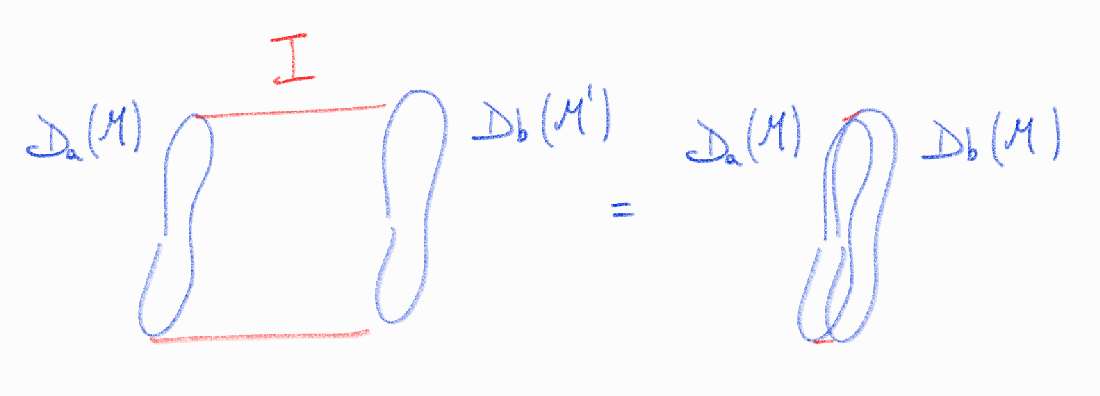
\includegraphics[width=0.75\linewidth]{images/11 parallel fusion_260702_165948.pdf}
    \caption{Parallel collision of two codimension-$(p+1)$ topological defects $\mathcal{D}_a$ and $\mathcal{D}_b$ across an interval $I$, fusing into a linear combination of simple defects.}
    \label{fig:fusion_geometry}
\end{figure}

Because the operators are strictly topological, correlation functions are invariant under variations of the distance separating them, provided no non-topological local operators are inserted within the intervening spacetime interval $I$. Taking the limit as the interval collapses yields the fusion product $\mathcal{D}_a \times \mathcal{D}_b$. Crucially, this operation generally lacks an inverse, separating generalized symmetries from traditional group-like structures.

In an arbitrary spacetime dimension $d$, the fusion rules take the general form:
\begin{equation}
    \mathcal{D}_a \times \mathcal{D}_b = \sum_c \mathcal{Z}^c_{ab} \mathcal{D}_c
\end{equation}
where the operators $\mathcal{D}_i$ form a basis of simple topological symmetry operators. The coefficients $\mathcal{Z}^c_{ab}$ represent the complex-valued partition functions of a lower-dimensional Topological Quantum Field Theory (TQFT) evaluated on the manifold where the fusion occurs \cite{Roumpedakis_2023}. In the well-established $2d$ case, these coefficients collapse to non-negative integers ($\mathcal{Z}^c_{ab} \in \mathbb{N}$), dictating the multiplicity of the fused channels.

\paragraph{The sum:}
For any two symmetry operators $\mathcal{D}_a$ and $\mathcal{D}_b$, we can define a formal sum $\mathcal{D}_a + \mathcal{D}_b$ such that the line relation satisfies linear superposition at the level of the path integral: $\langle [\mathcal{D}_a + \mathcal{D}_b] \dots \rangle = \langle \mathcal{D}_a \dots \rangle + \langle \mathcal{D}_b \dots \rangle$.

A structural refinement of this operation is required when distinguishing between general topological operators and genuine topological defect operators, as detailed in \ref{sec:topo_op-vs-symm_op}.\footnote{Local topological operators ($(d-1)$-form symmetries) and spacetime-filling topological operators (($-1$)-form symmetries) constitute structural exceptions to this framework. Spacetime-filling operators wrap the entire manifold, preventing them from trapping a localized cycle to twist the state space on a lower-dimensional slice; instead, they projectively decouple the full path integral.} At the state level, the twisted Hilbert space $\mathcal{H}_{\mathcal{D}_a + \mathcal{D}_b}$ associated with a formal sum of defects decomposes directly into the direct sum of the individually twisted Hilbert spaces:
\begin{equation}
    \mathcal{H}_{\mathcal{D}_a + \mathcal{D}_b} = \mathcal{H}_{\mathcal{D}_a} \oplus \mathcal{H}_{\mathcal{D}_b}
\end{equation}

\subsection{Simple vs non-simple topological operators} \label{sec:simple_topo_op}

To systematically classify the basis elements of this defect space, we introduce the concept of simple topological operators \cite{shao2024whatsundonetasilectures, schafernameki2023ictplecturesnoninvertiblegeneralized}.

A topological defect $\mathcal{D}$ is structurally simple if its endomorphism algebra—defined as the space of worldvolume local operators $\text{Hom}(\mathcal{D}, \mathcal{D})$—is isomorphic to $\mathbb{C}$, containing no topological point insertions other than the identity $\mathbb{I}_{\mathcal{D}}$. If $\dim \text{Hom}(\mathcal{D}, \mathcal{D}) > 1$, the operator is non-simple and splits into a direct sum of simple components. Physical fusion products of simple defects routinely yield non-simple defects, which manifest as a direct sum of distinct simple channels weighted by their quantum dimension.

\subsection{Higher fusion categories as symmetry structures}

The comprehensive mathematical framework required to organize these nested structures of simple and non-simple extended defects across multiple dimensions is higher category theory \cite{schafernameki2023ictplecturesnoninvertiblegeneralized}.

\begin{tcolorbox}
{\bf Category Theory: Structural Intuition}

Category theory abstractly formalizes mathematical structures and their valid transformations. A category comprises a collection of {\it objects} and {\it morphisms} (arrows) acting between them, ensuring compatibility with the underlying axioms of the structural class.

For instance, the categories {\bf Set}, {\bf Grp}, {\bf Diff}, and {\bf Bun} classify sets, groups, differentiable manifolds, and fiber bundles, respectively. Their corresponding morphisms are functions, group homomorphisms, diffeomorphisms, and bundle maps. This framework allows for structural abstraction, mapping mathematical theorems across disparate fields without relying on the internal composition of the underlying objects.

{\it Higher category theory} extends this principle by treating the morphisms themselves as objects. It introduces $2$-morphisms as directed maps between $1$-morphisms, iterating sequentially to $n$-categories.
\end{tcolorbox}

In the context of quantum field theory, the full generalized global symmetry structure is captured by a higher fusion category $\mathcal{S}$. The objects ($0$-morphisms) correspond to the top-dimensional ($(d-1)$-dimensional) topological operators in the theory. The higher $k$-morphisms track the lower-dimensional topological defects that reside as junctions, boundaries, or interfaces between the higher-dimensional operators \cite{schafernameki2023ictplecturesnoninvertiblegeneralized}. Look at FIG. \ref{fig:higher_category_defects}.

\begin{tcolorbox}[colback=green!5!white, colframe=green!75!black, title={Example: Symmetry Structure in a $3d$ QFT}]
In a $3d$ spacetime, the generalized global symmetry structure is organized into a fusion $2$-category:\footnote{To fully unify the paradigm, $(-1)$-form symmetries can be integrated into the higher categorical framework as top-dimensional modifications or decorations that parameterize the choice of the fusion category instance itself. In fact, that would describe families of QFTs instead of a single one.}
\begin{enumerate}[\itshape i)]
    \item {\bf Topological Surfaces $\mathcal{D}_2$ ($0$-morphisms):} The codimension-$1$ objects that generate the standard $0$-form global symmetry.
    \item {\bf Topological Lines $\mathcal{D}_1$ ($1$-morphisms):} The codimension-$2$ defects that function both as standalone generators of $1$-form symmetries and as topological interfaces between distinct $\mathcal{D}_2$ surfaces.
    \item {\bf Topological Point Operators $\mathcal{D}_0$ ($2$-morphisms):} The codimension-$3$ operators that generate $2$-form symmetries and act as junctions where lines terminate or intersect.
\end{enumerate}
At each nested categorical level, the composition laws are dictated by non-invertible fusion rules.
\end{tcolorbox}

\begin{figure}
    \centering
    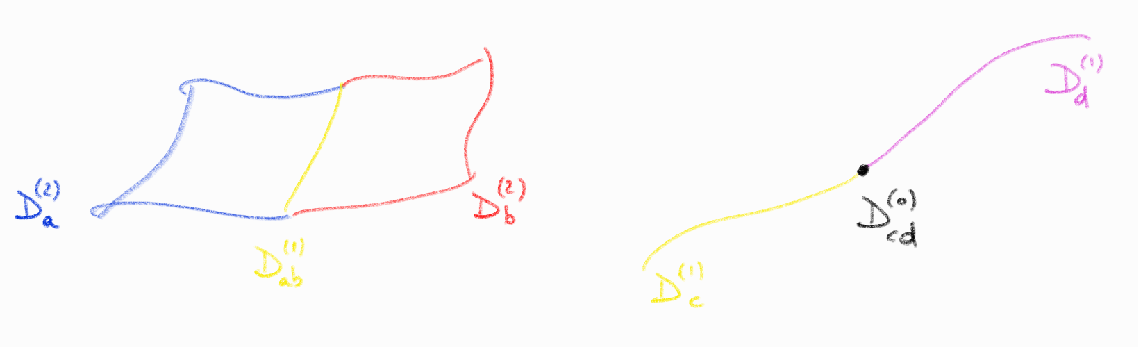
\includegraphics[width=1\linewidth]{images/12 category_260702_170243.pdf}
    \caption{Geometric nested structure of a fusion $2$-category in $3d$: topological point operators ($\mathcal{D}_0$) acting as junctions on topological lines ($\mathcal{D}_1$), which bound or separate topological symmetry surfaces ($\mathcal{D}_2$).}
    \label{fig:higher_category_defects}
\end{figure}

\begin{tcolorbox}[colback=green!5!white, colframe=green!75!black, title={Example: Invertible $0$-Form Group Symmetry}]
In a $2d$ QFT possessing an invertible $0$-form global group symmetry $G$, the symmetry structure simplifies to the fusion category of $G$-graded vector spaces:
\begin{equation}
    \mathcal{S} = \text{Vec}_G
    \label{eq:vec_g}
\end{equation}
The simple objects are $1d$ topological lines labelled by $g \in G$, and their fusion maps directly to the group multiplication. The dual charged local operators are classified by the representation category $\text{Rep}(G)$.

In a $3d$ QFT with the same $0$-form group symmetry $G$, the structure escalates to a fusion $2$-category denoted as $\text{2-Vec}_G$. Here, the simple objects are topological surfaces wrapped on spatial cycles, while the $1$-morphisms and $2$-morphisms dictate the topological line and point defects allowed to live on their worldvolumes.
\end{tcolorbox}

\subsection{Topological Local Operators and Dual Symmetry Operators}
\label{sec:topo_loc_op}

When evaluating a $(d-1)$-form global symmetry, the corresponding topological symmetry operators collapse to $0$-dimensional manifolds, manifesting physically as {\bf topological local operators}. If the symmetry is finite and group-like, it triggers the phenomenon of {\bf decomposition} \cite{McGreevy_2023, vandermeulen2022lowerformsymmetries}. The parent theory $\mathcal{T}_D$ breaks up into a direct sum of completely decoupled sectors called ``universes'':
\begin{equation}
    \mathcal{T}_D = \bigoplus_i \mathcal{T}_i \implies \mathcal{Z}_{\mathcal{T}_D} = \sum_i \mathcal{Z}_{\mathcal{T}_i}
\end{equation}
The topological local operators act as orthogonal projection operators $\mathcal{D}_i$ onto these individual universes, satisfying an idempotent, non-group-like fusion algebra:
\begin{equation}
    \mathcal{D}_i \otimes \mathcal{D}_j = \delta_{ij} \mathcal{D}_i
\end{equation}

Gauging this $(d-1)$-form symmetry projects the system onto a single universe, which uncovers a quantum dual {\bf $(-1)$-form global symmetry}.\footnote{The only possible gauging for $d-1$-form symmetries is flat gauging.} Because a $p$-form symmetry maps to topological defects on $(d-p-1)$-dimensional slices, a $(-1)$-form symmetry is generated by {\bf spacetime-filling defects} that wrap the entire manifold.

There are two complementary perspectives to understand a $(-1)$-form symmetry:
\begin{enumerate}[\itshape i)]
    \item {\bf The Decomposition View:} The $(-1)$-form symmetry acts dynamically on the theory itself, mapping one universe to another ($\mathcal{T}_i \to \mathcal{T}_j$). Gauging the $(-1)$-form symmetry reverses this process: it sums over all individual universes, reconstructing the parent theory $\mathcal{T}_D$ and restoring the $(d-1)$-form symmetry.
    \item {\bf The Parameter Space View:} The symmetry acts as a topological operation that shifts the defining parameters or coupling constants of the theory. We can visualize a family of QFTs fibered over a parameter space base; ordinary symmetries act fiber-wise (vertically), while the $(-1)$-form symmetry acts on the base space (horizontally):
    \begin{equation}
        \text{QFT}_{\theta} \longrightarrow U_{\theta, \theta'} \text{QFT}_{\theta'}
    \end{equation}
\end{enumerate}

We can bridge these two views: a theory with a $(-1)$-form symmetry away from decomposition (like 4D Yang-Mills with a $\theta$-angle) can be viewed as an individual universe labeled by a specific parameter value. To treat the parameter topologically, we promote it to a spacetime-dependent background field, $\theta(x)$, which couples to a Chern-Weil-type current (a composite current, as mentioned in \ref{sec:superfluid_00_composite}). 

Ultimately, a theory possesses a $(-1)$-form symmetry because it is secretly a single universe of a decomposing parent theory. 

\paragraph{SymTFT Realization of $(-1)$-Form Symmetries:}

In the SymTFT framework, parameters and shifting operations cease to be intrinsic background artifacts; they are actively engineered by choosing specific topological boundary conditions and inserting codimension-one defects in the $(d+1)$-dimensional bulk. This geometric formulation unifies the parameter space and decomposition perspectives through three distinct structural mechanisms:

\begin{enumerate}[\itshape i)]
    \item {\bf Topological Point Operators (TPOs) and Parameter Shifts:} When the bulk action admits TPOs ($W_\beta$), they link non-trivially with dual codimension-one defects ($U_\alpha$). Inserting a $U_\alpha$ defect parallel to a chosen symmetry boundary condition $\langle N_\theta|$ shifts the defining background parameter:
    \begin{equation}
        \langle N_\theta| U_\alpha = \langle N_{\theta+\alpha}|
    \end{equation}
    This shift maps the system from one distinct universe to another. Gauging this $(-1)$-form symmetry amounts to constructing a non-simple symmetry boundary via a formal direct sum of these shifted boundaries, $\bigoplus_k \langle N_{\theta + k\alpha}|$, which explicitly triggers decomposition in the absolute theory.

    \item {\bf Condensation Defects and Higher Gauging:} When the bulk lacks intrinsic TPOs, $(-1)$-form symmetries are engineered via higher gauging. In this setup, codimension-one condensation defects are constructed by condensing lower-dimensional extended operators. Colliding these defects with the boundary alters the boundary conditions or modulates continuous parameters.

    \item {\bf Non-Invertible Defects and Boundary Non-Simplicity:} Non-invertible $(-1)$-form symmetries manifest as bulk codimension-one defects ($S_e, S_m$) obeying fusion rules weighted by internal TQFT partition functions. Acting with these defects transmutes a simple boundary condition into a non-simple one.
    
    Geometrically, this allows bulk line operators to terminate on the defect interface. When collapsed, this interface generates a dense set of topological local operators on the boundary, mapping a single universe into a decomposing direct sum of superselection sectors.
\end{enumerate}

\subsection{Interlude D: Genuine and non-genuine operators}
\label{sec:genuine_op}

To characterize the full spectrum of observables in a generalized symmetry framework, we must classify operators by their topological independence. 

An operator $\mathcal{O}(\mathcal{M}_p)$ supported on a $p$-dimensional submanifold $\mathcal{M}_p$ is defined as \textbf{genuine} if its correlation functions depend exclusively on the geometry and topology of $\mathcal{M}_p$. It exists independently of any other higher-dimensional structures in the spacetime bulk. 

Conversely, an operator $\mathcal{O}'(\mathcal{M}_p)$ is \textbf{non-genuine} if it cannot stand alone; it requires the choice of a higher-dimensional topological surface $\Sigma_{p+1}$ such that $\mathcal{M}_p$ forms its boundary:
\begin{equation}
    \partial \Sigma_{p+1} = \mathcal{M}_p
\end{equation}
Non-genuine operators physically manifest as boundary excitations, endpoints, or junction defects where higher-dimensional topological symmetry operators terminate. When gauging a global symmetry, genuine operators that are not invariant under the gauge group are projected out, while formerly non-genuine operators attached to the boundaries of newly topological gauge-surface defects become well-defined, genuine line or surface observables in the gauged theory.

\subsection{Interlude E: Topological operators vs symmetry defects} 
\label{sec:topo_op-vs-symm_op}

The distinction between a topological operator and a symmetry defect is fundamentally geometric, dictated by the orientation of the defect's worldvolume relative to the foliation of Euclidean spacetime. This dual nature is formalized by the \textit{operator-defect principle} \cite{shao2024whatsundonetasilectures}.

Consider a codimension-$(p+1)$ topological operator living on a manifold $\mathcal{M}_{d-p-1}$. The physical interpretation depends on its embedding:
\begin{enumerate}[\itshape i)]
    \item \textbf{The Operator Perspective:} When $\mathcal{M}_{d-p-1}$ is embedded entirely within a constant-time slice $\Sigma_{d-1}$, it acts as a topological state-space operator on the untwisted Hilbert space $\mathcal{H}$. Sweeping this operator past local or extended insertions implements a symmetry transformation via the standard higher-dimensional Ward identities.
    \item \textbf{The Defect Perspective:} When $\mathcal{M}_{d-p-1}$ wraps a cycle that extends along the Euclidean time direction $S^1_\tau$, it modifies the global quantization conditions. It acts as a static background field insertion that intersects the spatial slices, structurally altering the spatial boundary conditions and forcing the state space into a \textbf{twisted Hilbert space} $\mathcal{H}_{\mathcal{D}}$.
\end{enumerate}

In conformal field theories (CFTs), modular invariance enforces a strict consistency condition between these two views \cite{McGreevy_2023}. On a torus $T^2$, an $\mathcal{S}$-duality transformation swaps the spatial and temporal cycles. This geometric rotation maps a topological operator acting on states directly to a background symmetry defect generating a twisted sector, proving that the spectrum of operators and the spectrum of twisted states are rigidly bound by modular bootstrap constraints.

\subsection{Interlude F: The Generalized Landau Paradigm} 
\label{sec:landau_paradigm}

The classical Landau paradigm classifies phases of matter and their transitions via the expectation values of local order parameters $\langle \mathcal{O}(x) \rangle$ that spontaneously break a $0$-form global symmetry group. The generalized Landau paradigm extends this diagnostic classification to higher-form and non-invertible symmetries by substituting local operators with extended topological defects \cite{McGreevy_2023}.

For a $1$-form symmetry, the physical phase of the theory is probed by the asymptotic scaling behavior of an extended charged object, such as a closed Wilson loop $W(\mathcal{C})$ or a dual 't Hooft operator $H(\mathcal{M}_{d-3})$ wrapped on a manifold of characteristic linear size $L$:
\begin{enumerate}[\itshape i)]
    \item \textbf{Area Law (Unbroken Symmetry $\implies$ Confinement):} An expectation value scaling with the minimal area enclosed by the loop indicates a disordered phase where the $1$-form global symmetry remains strictly unbroken:
    \begin{equation}
        \langle W(\mathcal{C}) \rangle \sim \exp\left( -\sigma \cdot \text{Area}(\mathcal{C}) \right)
    \end{equation}
    where $\sigma$ is the non-vanishing string tension. This behavior provides a rigorous, symmetry-based definition of \textbf{confinement}: isolated fundamental test charges possess infinite energy, as the flux tubes connecting them cannot break due to the absence of dynamical screening matter.
    \item \textbf{Perimeter Law (Spontaneous Symmetry Breaking $\implies$ Deconfinement):} A scaling that depends exclusively on the perimeter of the contour indicates a screened or deconfined phase:
    \begin{equation}
        \langle W(\mathcal{C}) \rangle \sim \exp\left( -\alpha \cdot \text{Perimeter}(\mathcal{C}) \right)
    \end{equation}
    By performing a topological counterterm subtraction, this perimeter dependence can be localized, leaving a non-zero constant expectation value. This signifies that the $1$-form global symmetry is spontaneously broken. The low-energy spectrum in this phase is characterized either by long-range topological order (discrete gauge theories) or by massless Goldstone bosons, such as the photon in a deconfined Coulomb phase.
\end{enumerate}

\subsection{Interlude G: Consequences of generalized symmetries} 
\label{sec:consequences_of_gensym}

Generalized and non-invertible symmetries impose strict, non-perturbative constraints on the dynamics of quantum field theories, severely restricting the infrared (IR) endpoints of Renormalization Group (RG) flows.

A critical consequence is the circumvention of classical anomaly-breaking arguments via non-invertible chiral symmetries \cite{choi2022noninvertibleglobalsymmetriesstandard, cordova2022noninvertiblechiralsymmetryexponential}. In standard $4d$ gauge theories, the Adler-Bell-Jackiw (ABJ) anomaly breaks the invertible $U(1)_A$ axial symmetry down to a discrete subgroup by coupling the axial current divergence to the topological charge density $F \wedge F$. However, by stacking the spacetime bulk with a lower-dimensional fractional quantum Hall TQFT coupled to the gauge curvature living in the physical theory, one constructs a non-invertible topological chiral symmetry operator $\mathcal{D}_a$.

Because these generalized symmetry operators are strictly conserved, they yield exact multi-point selection rules on Euclidean correlation functions. They protect light degrees of freedom by explicitly forbidding mass terms for fermions or Nambu-Goldstone bosons: a non-zero mass would induce an explicit exponential decay in correlators that violates the categorical conservation laws. Consequently, non-invertible symmetries guarantee exact masslessness or enforce specific, non-trivial matching anomalies that require the theory to flow to either a gapless phase or a topological low-energy state.

\paragraph{Energy Scale Hierarchies in Higher-Groups:}
When global symmetries mix into a higher-group structure, such as a $2$-group, the symmetry breaking dynamics become rigidly coupled across distinct energy scales. In a $2$-group, the background gauge fields $B_1$ of a $0$-form symmetry $G$ and $B_2$ of a $1$-form symmetry $A$ satisfy a non-trivial transformation law detailed by the structure equation:
\begin{equation}
    \delta B_2 = e \cdot H^3(B_1)
\end{equation}
where $e$ represents the Postnikov class. 

This structural mixing prevents the independent, arbitrary setting of symmetry-breaking scales. If the $0$-form symmetry $G$ undergoes spontaneous symmetry breaking at an energy scale $f_0$, the non-triviality of the Postnikov class $e$ structurally restricts the dynamics of the $1$-form symmetry. Specifically, the theory cannot transition into a phase where $G$ is broken while $A$ remains unbroken at a higher scale. This establishes a strict energy scale inequality:
\begin{equation}
    \Lambda_{\text{SSB}}^{(1\text{-form})} \leq \Lambda_{\text{SSB}}^{(0\text{-form})}
\end{equation}
The breaking of the $0$-form symmetry at $f_0$ induces an explicit modification of the effective topological sectors available to the $1$-form symmetry fields in the IR. Consequently, the high-energy breaking of the lower-form symmetry triggers or bounds the modification of the higher-form symmetry structures, forcing a strict hierarchy of phase transitions within the low-energy effective field theory.

\newpage
%---------------------------------------------------------
\section{Anomalies}
%---------------------------------------------------------

In the Hamiltonian formalism, 't Hooft anomalies manifest as the impossibility of lifting a classical global symmetry group $G$ to a linear representation on the Hilbert space, forcing the quantum states to furnish a projective representation instead. In the modern framework where global symmetries are identified with topological operators, an anomaly corresponds to the failure of the topological property when the system is coupled to a background field for another (or the same) symmetry \cite{McGreevy_2023}. 

Concretely, an anomaly implies that certain topological operators play a dual role: they act simultaneously as symmetry generators and as charged operators, meaning they are not invisible to the action of other symmetry operators.

In this thesis, we will refer to pure 't Hooft anomalies as simply pure anomalies, and similarly for mixed anomalies. Other concepts traditionally termed anomalies (such as ABJ or gauge anomalies) represent distinct physical phenomena; a precise clarification of this terminology is provided below.

\begin{tcolorbox}
{\bf General Idea of a 't Hooft Anomaly} \\
Given a $d$-dimensional QFT $\mathcal{T}$ possessing a global symmetry group $G$, we can couple the theory to a classical background gauge field $B$. The theory exhibits a 't Hooft anomaly if the partition function $\mathcal{Z}[B]$ is not invariant under background gauge transformations $B \to B^g$:
\begin{equation}
    \mathcal{Z}[B^g] = \mathcal{Z}[B] \times \exp \left( i \int_{\mathcal{M}_d} \alpha(B, \lambda) \right)
\end{equation}
where $B^g = B + d\lambda$ for continuous symmetries, and $B^g = B + \delta\lambda$ for discrete symmetries. Crucially, this non-invariance cannot be removed by adding any local counterterm to the action. A direct consequence is that the theory $\mathcal{T}$ does not admit dynamical gauging with respect to the anomalous symmetry group $G$.
\end{tcolorbox} 

\subsection{Clarification of the Terminology}
In the literature, it is common to encounter the terms "'t Hooft anomaly", "mixed 't Hooft anomaly", "ABJ anomaly", and "gauge anomaly". Let us clarify the differences between these concepts:
\begin{enumerate}[\itshape i)]
    \item \textbf{'t Hooft anomaly (Pure/Mixed):} An obstruction to gauging a global symmetry by turning on classical background fields. It is a robust feature of the theory and an RG-flow invariant, meaning it must be matched identically between the UV and the IR. In $4d$ gauge theories with continuous gauge groups, perturbative 't Hooft anomalies are computed from triangle diagrams having global symmetry currents on all three vertices.
    \item \textbf{Gauge anomaly:} An inconsistency in a theory where a gauge transformation of dynamical gauge fields does not leave its contribution to the path integral invariant. Since gauge symmetries are redundancies of the description rather than physical global symmetries, a gauge anomaly renders the theory mathematically ill-defined. In $4d$, the corresponding triangle diagrams have dynamical gauge currents on all three vertices.
    \item \textbf{ABJ anomaly:} A phenomenon occurring when a transformation is a symmetry of the classical Lagrangian, but fails to be a symmetry of the full quantum partition function due to the non-invariance of the path integral measure. Such a transformation is not a true global symmetry of the QFT. In $4d$, ABJ anomalies are characterized by triangle diagrams having gauge currents on two vertices and a global current on the third vertex. Gaugining a non-anomalous subgroup of a theory with a mixed 't Hooft anomaly yields an ABJ anomaly for the remaining global factor.
\end{enumerate}

\paragraph*{Non-anomalous situation:} Given a theory possessing a group-like symmetry, we can couple it to a background field $B$ by inserting its Noether current $\star j$:
\begin{equation}
    \mathcal{Z}[B] = \int \mathcal{D}\phi \exp \left( -S[\phi] + i \int \star j(\phi) \wedge B \right)
\end{equation}
In the non-anomalous case, the invariance of $\mathcal{Z}$ under background gauge transformations $B \to B + d\Lambda$ reads:
\begin{equation}
    \mathcal{Z}[B + d\Lambda] = \mathcal{Z}[B] \iff \int \mathcal{D}\phi \exp \left( i \int \star j(\phi) \wedge d\Lambda \right) = 1
\end{equation}
Integrating by parts, this requires $d\star j=0$. This invariance ensures that the symmetry can be dynamically gauged, as the partition function is well-defined on the cohomology class of $B$.

\paragraph*{Pure 't Hooft anomaly:} A pure anomaly occurs when the partition function picks up a classical background-dependent phase factor under gauge transformations:
\begin{equation}
\label{eq:pure_anomaly}
    \mathcal{Z}[B + d\Lambda] = \exp\left(i \int_{\mathcal{M}_d} \alpha(B, \Lambda)\right) \times \mathcal{Z}[B] 
\end{equation}
where the phase factor prevents $\mathcal{Z}[B]$ from being a well-defined function on the cohomology class $[B]$, obstructing dynamical gauging even after adding local counterterms.

\paragraph*{Mixed 't Hooft anomaly:} A mixed anomaly is a configuration where the global symmetry group splits into distinct factors, such as a $p$-form symmetry and a $q$-form symmetry. Coupling the system to the respective background fields $B_{p+1}$ and $B_{q+1}$, the partition function is invariant under individual transformations:
\begin{equation}
    \mathcal{Z}[B_{p+1}^g, B_{q+1}] = \mathcal{Z}[B_{p+1}, B_{q+1}] \qquad \text{and} \qquad \mathcal{Z}[B_{p+1}, B_{q+1}^g] = \mathcal{Z}[B_{p+1}, B_{q+1}]
\end{equation}
However, the simultaneous transformation yields a non-trivial mutual phase factor that cannot be fixed by local counterterms of both fields:
\begin{equation}
    \mathcal{Z}[B_{p+1}^g, B_{q+1}^g] = \exp\left(i \int_{\mathcal{M}_d} \beta(B_{p+1}, \Lambda_p, B_{q+1}, \Lambda_q)\right) \times \mathcal{Z}[B_{p+1}, B_{q+1}] 
\end{equation}
Physically, this indicates that while the two symmetries can be gauged individually, they cannot be dynamically gauged at the same time.

\begin{tcolorbox}[colback=green!5!white, colframe=green!75!black, title={Example: Maxwell Theory}]
    Consider a $d$-dimensional pure $U(1)$ gauge theory coupled to continuous background fields $B_2^e$ and $B_{d-2}^m$ for the electric $1$-form and magnetic $(d-3)$-form symmetries respectively. Performing an electric gauge transformation $B_2^e \to B_2^e + d\Lambda_1^e$ shifts the action by $\Delta S = 2\pi \int \Lambda_1^e \wedge d\star F$. Since the magnetic background modifies the Maxwell equation to $d\star F = -dB_{d-2}^m$, the partition function transforms as:
\begin{equation}
    \mathcal{Z}[B_2^e + d\Lambda_1^e, B_{d-2}^m] = \exp\left(-2\pi i \int \Lambda_1^e \wedge dB_{d-2}^m\right) \times \mathcal{Z}[B_2^e, B_{d-2}^m]
\end{equation}
Interchanging the roles and transforming the magnetic background via $B_{d-2}^m \to B_{d-2}^m + d\Lambda_{d-3}^m$ yields:
\begin{equation}
    \mathcal{Z}[B_2^e, B_{d-2}^m + d\Lambda_{d-3}^m] = \exp\left(2\pi i \int dB_2^e \wedge \Lambda_{d-3}^m\right) \times \mathcal{Z}[B_2^e, B_{d-2}^m]
\end{equation}
This establishes a continuous mixed 't Hooft anomaly between the electric and magnetic higher-form sectors.
\end{tcolorbox}


\subsection{Description in terms of Topological Operators}
For discrete symmetries, gauge transformations of background fields are geometrically equivalent to deformations of the topological defects generating those symmetries. A 't Hooft anomaly arises when such deformations change the correlation functions, which occurs when topological defects or their junctions cross each other. This implies that the topological operators or their junctions carry non-trivial charges under the symmetry itself.

\paragraph*{Example: Discrete Gauge Theories.} For a discrete gauge theory with background fields $B_{p+1}^e$ and $B_{d-p}^m$, a discrete electric gauge transformation $B_{p+1}^e \to B_{p+1}^e + \delta \Lambda_p^e$ shifts the partition function as:
\begin{equation}
    \mathcal{Z}[B_{p+1}^e + \delta \Lambda_p^e, B_{d-p}^m] = \exp\left(2\pi i (-1)^p \int \Lambda_p^e \cup_{\eta} B_{d-p}^m\right) \times \mathcal{Z}[B_{p+1}^e, B_{d-p}^m]
\end{equation}
Conversely, a magnetic gauge transformation $B_{d-p}^m \to B_{d-p}^m + \delta \Lambda_{d-p-1}^m$ yields:
\begin{equation}
    \mathcal{Z}[B_{p+1}^e, B_{d-p}^m + \delta \Lambda_{d-p-1}^m] = \exp\left(-2\pi i \int B_{p+1}^e \cup_{\eta} \Lambda_{d-p-1}^m\right) \times \mathcal{Z}[B_{p+1}^e, B_{d-p}^m]
\end{equation}
This anomaly occurs because the topological operators constituting the electric $p$-form symmetry are charged under the magnetic $(d-p-1)$-form symmetry, and vice versa. Deforming a magnetic operator sweeps out a $(p+1)$-chain Poincaré dual to $\Lambda_{d-p-1}^m$. As it crosses the background network of electric operators, the intersection generates the topological phase factor $\exp\left(-2\pi i \int B_{p+1}^e \cup_{\eta} \Lambda_{d-p-1}^m\right)$.

\subsubsection{Anomaly inflow and anomaly polynomials}
The non-invariance of the partition function under background gauge transformations can be physically resolved by viewing the $d$-dimensional anomalous theory $\mathcal{T}$ as living on the boundary of a $(d+1)$-dimensional auxiliary bulk. This mechanism is known as \textit{anomaly inflow}.

To compensate for the phase factor in \ref{eq:pure_anomaly} without introducing unphysical bulk degrees of freedom, we couple $\mathcal{T}$ to a $(d+1)$-dimensional invertible topological field theory $\mathcal{A}_{D+1}[B]$, termed the \textit{anomaly theory} (which physically corresponds to a Symmetry Protected Topological, or SPT, phase).\footnote{An SPT phase in spatial dimension $d+1$ has a global symmetry $G$ such that, when placed on a manifold with boundary, the $d$-dimensional theory on the boundary has a ’t Hooft anomaly for $G$.} Let $\mathcal{M}_d = \partial \mathcal{M}_{D+1}$. The bulk partition function $\mathcal{Z}_{\mathcal{A}_{D+1}}[B]$ is well-defined on closed manifolds, but on a manifold with a boundary it transforms under background gauge transformations with the exact inverse phase of the boundary theory:
\begin{equation}
    \mathcal{Z}_{\mathcal{A}_{D+1}}[B^g] = \exp\left(-i \int_{\mathcal{M}_d} \alpha(B, \Lambda)\right) \times \mathcal{Z}_{\mathcal{A}_{D+1}}[B]
\end{equation}
By defining the total, coupled partition function as:
\begin{equation}
    \widetilde{\mathcal{Z}}[B] = \mathcal{Z}_{\mathcal{T}}[B] \times \mathcal{Z}_{\mathcal{A}_{D+1}}[B]
\end{equation}
full background gauge invariance is restored, $\widetilde{\mathcal{Z}}[B^g] = \widetilde{\mathcal{Z}}[B]$, at the price of rendering the system a boundary condition for a higher-dimensional bulk.

For continuous symmetries, the effective action $\mathcal{S}_{D+1} = \int \omega_{D+1}$ of the anomaly theory defined via $\mathcal{A}_{D+1}[B] = \exp(2\pi i \mathcal{S}_{D+1})$ can be systematically tracked via a $(d+2)$-dimensional invariant differential form called the \textit{anomaly polynomial} $\mathcal{I}_{d+2}$.

The relationship between the $(d+2)$-dimensional anomaly polynomial, the $(d+1)$-dimensional bulk action, and the $d$-dimensional phase variation is governed by the \textit{descent procedure}. 

Because $\mathcal{I}_{d+2}$ is closed ($d\mathcal{I}_{d+2} = 0$), it can be locally written as the exterior derivative of a $(d+1)$-form $\omega_{D+1}(B)$:\footnote{This is a notorious ambiguous step, the $\omega_{D+1}$ we obtain is not unique. This means that we can have multiple different presentation of the same anomaly.}
\begin{equation}
    \mathcal{I}_{d+2} = d\omega_{D+1}(B)
\end{equation}
Under a background gauge transformation, the gauge invariance of $\mathcal{I}_{d+2}$ ($ \delta_{\Lambda} \mathcal{I}_{d+2} = 0 $) implies that the variation of the $d+1$-form must be an exact form:
\begin{equation}
    \delta_{\Lambda} \omega_{D+1}(B) = d\alpha_d(B, \Lambda)
\end{equation}
The bulk anomaly theory is then defined by integrating the $\omega_{D+1}$ form over the $(d+1)$-dimensional manifold:
\begin{equation}
    \mathcal{A}_{D+1}[B] = \exp\left( 2\pi i \int_{\mathcal{M}_{D+1}} \omega_{D+1}(B) \right)
\end{equation}
Applying Stokes' theorem, the gauge variation of the bulk action reduces entirely to a boundary integral:
\begin{equation}
    \delta_{\Lambda} \int_{\mathcal{M}_{D+1}} \omega_{D+1}(B) = \int_{\mathcal{M}_{D+1}} d\alpha_d(B, \Lambda) = \int_{\mathcal{M}_d} \alpha_d(B, \Lambda)
\end{equation}
This boundary term matches the phase variation $\alpha(B, \Lambda)$ in \ref{eq:pure_anomaly}, demonstrating how the descent procedure mathematically tracks the inflow of anomalous charge from the bulk to the boundary.


  

%\begin{tcolorbox}[colback=gray!5, colframe=black, title={\bf Infrared Constraints from Anomalies}]
\begin{tcolorbox}
{\bf Infrared Constraints from Anomalies}

The presence of a 't Hooft anomaly yields severe constraints on the low-energy behavior of a quantum field theory under the renormalization group (RG) flow. Because 't Hooft anomalies are completely invariant under the RG flow, the anomaly computed in the UV must match the anomaly of the effective theory in the IR. This matching requirement dictates that a theory carrying a non-trivial anomaly cannot flow to a trivial gapped phase in the infrared. Specifically, the IR phase diagram must satisfy at least one of the following scenarios:
\begin{enumerate}[\itshape i)]
    \item \textbf{Conformal Phase:} The theory flows to an IR non-trivial Fixed Point, governed by a gapless Conformal Field Theory (CFT).
    \item \textbf{Spontaneous Symmetry Breaking (SSB):} The anomalous global symmetry is spontaneously broken, implying the presence of gapless Goldstone modes (for continuous symmetries) or a degenerate topological ground state lattice (for discrete symmetries).
    \item \textbf{Topological Order:} The theory flows to a non-trivial gapped Topological Quantum Field Theory (TQFT) that captures and matches the anomaly via an emergent topological sector or fractionalized excitations.
\end{enumerate}
In the language of generalized higher-form symmetries, this matching condition acts as an absolute obstruction to a unique, trivial gapped vacuum, forcing the infrared dynamics to either retain gapless degrees of freedom or support non-trivial topological defects.
\end{tcolorbox}

\subsection{Interlude H: Hydrodynamics and Generalized Symmetries}
\label{sec:hydro}

Hydrodynamics is not merely a model of fluid behavior; it is the universal effective field theory (EFT) governing long-wavelength fluctuations at finite temperature, entirely constrained and dictated by the global symmetries of the underlying system \cite{McGreevy_2023, iqbal2025jenalecturesgeneralizedglobal}. In this framework, the only persistent infrared (IR) degrees of freedom are the conserved currents and the gapless modes associated with them.

The modern microscopic origin of these hydrodynamic degrees of freedom is explained within the Schwinger-Keldysh formalism at finite temperature \cite{Delacretaz_2025}:
\begin{enumerate}[\itshape i)]
    \item \textbf{Symmetry Duplication:} Formulating a QFT on a closed time path (the thermal double profile) duplicates every continuous global symmetry $G$ into a twin structure, $G_L \times G_R$, acting independently on the forward and backward time legs.
    \item \textbf{Thermal Spontaneous Symmetry Breaking:} The thermal state spontaneously breaks the relative (axial) combination of these duplicated symmetries down to the diagonal subgroup:
    \begin{equation}
        G_L \times G_R \longrightarrow G_{\text{diag}}
    \end{equation}
    The resulting Goldstone-like fluctuations of this thermal breaking pattern are precisely the dynamic displacement or phase fields that construct the hydrodynamic description. 
\end{enumerate}

This symmetry-centric formulation applies directly to generalized higher-form symmetries. For a theory possessing a continuous $1$-form global symmetry, the conserved quantity is a antisymmetric $2$-form current $J^{\mu\nu}$ obeying $\partial_{\mu} J^{\mu\nu} = 0$. At finite temperature, this $1$-form symmetry undergoes the same thermal duplication and partial breaking, generating gapless hydrodynamic string excitations.

\paragraph{Application to Magnetohydrodynamics (MHD):}\footnote{The theory of electrically charged fluids, as plasma, liquid metals or salt water.}
This framework provides a rigorous definition of magnetohydrodynamics without referencing fundamental dynamical photons. In a $4d$ plasma, the topological conservation of magnetic flux lines represents an exact $1$-form global symmetry whose current is dual to the field strength:
\begin{equation}
    J^{\mu\nu} = \frac{1}{2} \epsilon^{\mu\nu\rho\sigma} F_{\rho\sigma}
\end{equation}
The modes of plasma physics emerge purely as the gapless hydrodynamic excitations of this thermally broken $1$-form symmetry structure.

\paragraph{Limits of Validity}
The hydrodynamic derivative expansion is strictly valid only in the collisionless-to-hydrodynamic crossover regime where the fluctuation frequencies $\omega$ and wavevectors $k$ sit far below the thermalization scale set by the temperature:
\begin{equation}
    \omega \ll T, \quad |k| \ll T
\end{equation}
Crucially, because this mechanism relies on the duplication and continuous breaking of a continuous structure, it breaks down for discrete generalized symmetries (e.g., $\mathbb{Z}_N$). Discrete symmetries cannot generate continuous thermal Goldstone modes, meaning they do not contribute new hydrodynamic modes to the IR fluid picture.

\newpage 

\section{Mixed Anomalies and Their Gauging}
\label{sec:mixed_anomaly_to_gen_sym}

A mixed 't Hooft anomaly involving multiple global symmetries acts as a structural obstruction to their simultaneous dynamical gauging. When a subsector of the global symmetry structure is gauged, this classical obstruction undergoes a fundamental transformation: the variation of the partition function changes from a classical c-number background shift into an operator-valued quantum equation of motion constraint. Depending on the algebraic structure of the anomaly polynomial, this mechanism leads either to higher-group symmetries or to non-invertible topological defects \cite{Kaidi_2022, Bhardwaj_2023, Antinucci_2025}.

\subsection{Continuous Symmetries and Higher-Group Formations}
\label{sec:continuous_higher_groups}

Consider a $4\text{D}$ field theory containing a $0$-form global symmetry $U(1)_A^{(0)}$ and a $1$-form global symmetry $U(1)_B^{(1)}$, with corresponding conserved currents $j^{(1)}_A$ and $j^{(2)}_B$. We couple these currents to the classical background fields $B_A$ (a $1$-form) and $B_B$ (a $2$-form) via the standard source term in the action:
\begin{equation}
    \mathcal{L} \supset \star j^{(1)}_A \wedge B_A + \star j^{(2)}_B \wedge B_B
\end{equation}
Suppose the system possesses a tame mixed anomaly such that the $1$-form symmetry current remains strictly closed, while the $0$-form current conservation law is explicitly modified by the background field strength of the companion symmetry \cite{Antinucci_2025}:
\begin{equation}
    d\star j^{(1)}_A = dB_A \wedge \star j^{(2)}_B \qquad \& \qquad d\star j^{(2)}_B = 0
\end{equation}
To evaluate the gauge invariance of the effective action under generic background variations $\delta B_A = d\Lambda_A$ and $\delta B_B = d\Lambda_B + K$, we compute the total variation of the Lagrangian density:
\begin{equation}
    \delta \mathcal{L} = \star j^{(1)}_A \wedge d\Lambda_A + \star j^{(2)}_B \wedge (d\Lambda_B + K)
\end{equation}
Integrating by parts and applying the modified conservation equations yields:
\begin{equation}
    \delta \mathcal{L} = -d\star j^{(1)}_A \wedge \Lambda_A - d\star j^{(2)}_B \wedge \Lambda_B + \star j^{(2)}_B \wedge K
\end{equation}
\begin{equation}
    \delta \mathcal{L} = -(dB_A \wedge \star j^{(2)}_B) \wedge \Lambda_A + \star j^{(2)}_B \wedge K
\end{equation}
Using the wedge product transpositions, this simplifies directly to:
\begin{equation}
    \delta \mathcal{L} = \star j^{(2)}_B \wedge \left( K - dB_A \wedge \Lambda_A \right)
\end{equation}
For the theory to preserve background gauge invariance off-shell ($\delta \mathcal{L} = 0$), the transformation of the higher-form background field must be non-trivially modified by the $0$-form parameters. This forces the constraint:
\begin{equation}
    K = dB_A \wedge \Lambda_A \implies \delta B_B = d\Lambda_B + dB_A \wedge \Lambda_A
\end{equation}
This interlocking transformation law defines a continuous $2$-group symmetry structure. The background fields can no longer be varied independently; instead, the $1$-form and $0$-form structures mix directly into what is called a higher-group.

\subsection{Discrete Gauging in the Presence of Anomalies}
\label{sec:discrete_gauging_anomalies}

When shifting from continuous fields to finite discrete symmetries, the consequences of gauging a non-anomalous subgroup are highly constrained by group cohomology. Following the general framework established by Tachikawa \cite{Tachikawa_2020}, let $\Gamma$ be a finite global symmetry group containing a normal, non-anomalous subgroup $A$. If we gauge $A$, the symmetry structure of the resulting quotient theory falls into one of three distinct classes depending on the nature of the original total 't Hooft anomaly:

\begin{enumerate}[\itshape i)]
    \item \textbf{Anomaly-Free / Trivial Case:} If the total group $\Gamma$ is anomaly-free, gauging $A$ yields a split symmetry group defined by the direct product of the quotient and the Pontryagin dual: $G \times \hat{A}$, where $G = \Gamma/A$. The gauged theory carries a purely discrete mixed anomaly determined by the topological extension class of $0 \to A \to \Gamma \to G \to 0$.
    \item \textbf{Tame Anomaly Case:} If the anomaly is non-vanishing but restricted to mild low-order topological sectors, the symmetry of the gauged theory does not split. Instead, it forms a non-trivial group extension of the ordinary symmetry $G$ by the higher-form Pontryagin dual symmetry $\hat{A}$, physically realizing a discrete higher-group structure.
    \item \textbf{Wild Anomaly Case:} If the mixed anomaly involves higher-degree topological invariants, local counterterms fail. Gauging $A$ completely destroys the group-like nature of the remaining transformations, forcing the matching observables to fuse according to a non-invertible higher-category symmetry structure.
\end{enumerate}

\subsection{Wild Anomalies and Non-Invertible Defects}
\label{sec:mix_anom_noninv_defect}

The physical mechanism driving the transition to non-invertible structures is the linear coupling of a background field within a higher-dimensional anomaly inflow action \cite{Kaidi_2022, Bhardwaj_2023, schafernameki2023ictplecturesnoninvertiblegeneralized}. 

Consider a $d$-dimensional theory with a $0$-form global symmetry $G^{(0)}$ and a $p$-form global symmetry $F^{(p)}$. Let their respective background fields be $A^{(1)}$ and $B^{(p+1)}$. Suppose the theory exhibits a mixed 't Hooft anomaly captured by a $(d+1)$-dimensional anomaly action linear in the $0$-form background:
\begin{equation}
    \mathcal{A}_{d+1} = \int_{\mathcal{M}_{d+1}} A^{(1)} \wedge f(B^{(p+1)})
\end{equation}
where $f$ maps the higher-form field to a $d$-form. 

A codimension-1 symmetry defect $\mathcal{D}(\mathcal{M}_{d-1})$ implementing a $G^{(0)}$ transformation is constructed by evaluating the partition function with a localized singular background $A^{(1)} = \delta(\mathcal{M}_{d-1})$. Due to the mixed anomaly, this defect is not invariant under the gauge transformations of the companion higher-form field $B^{(p+1)}$. To restore gauge invariance under the background transformations, the defect must be explicitly attached to a higher-dimensional bulk sector:
\begin{equation}
    \mathcal{D}(\mathcal{M}_{d-1}) \longrightarrow \mathcal{D}(\mathcal{M}_{d-1}) \times \exp \left( \int_{\mathcal{M}_d} f(B^{(p+1)}, \Lambda) \right) \qquad  \partial \mathcal{M}_d = \mathcal{M}_{d-1}
\end{equation}
If we now dynamically gauge the $G^{(0)}$ symmetry, the background field $A^{(1)}$ is promoted to a dynamical gauge field $a^{(1)}$. The anomaly term $a^{(1)} \wedge f(B^{(p+1)})$ can no longer be treated as a classical background phase. Instead, it acts as an explicit operator-valued violation of the $F^{(p)}$ symmetry current. 

Because the anomaly is linear in the gauged field, the defect $\mathcal{D}(\mathcal{M}_{D-1})$ transforms under the dynamical gauge group as an open boundary of a fractional topological sector. To make the defect well-defined and invariant under the dynamical gauge field $a^{(1)}$, we must stack a lower-dimensional topological quantum field theory (TQFT)—specifically a twisted fractional quantum Hall state or a discrete $\text{BF}$ action—directly onto the worldvolume $\mathcal{M}_{D-1}$. 

This explicit TQFT dressing restores topological conservation but alters the algebraic fusion rules. When two such dressed defects undergo a spatial collision, their internal TQFT degrees of freedom do not multiply like simple group elements. Instead, the fusion yields a sum over topological sectors, mathematically formalized as a condensation defect \cite{Roumpedakis_2023}:
\begin{equation}
    \mathcal{D}_g \times \mathcal{D}_g^\dagger = \mathcal{C} \neq \mathbf{1}
\end{equation}
The defect has become strictly non-invertible. This structural transition provides a universal prescription: whenever a background field for a $p$-form symmetry appears linearly in a mixed 't Hooft anomaly, gauging the complementary symmetries automatically converts the original invertible topological boundaries into non-invertible, category-valued symmetry operators in the gauged theory.

In the chapter \ref{sec:engineer_non-inv} you will see the explicit construction for cubic anomalies. It is clear that the result should be generalizable for quartic, quintic, etc. anomalies. We leave that for future works.

\subsection{Interlude I: Generalized Symmetries and Dynamical Gravity}
\label{sec:gravity_symmetries}

The holographic framework and the string theory landscape strongly support the swampland conjecture that exact global symmetries are strictly forbidden in quantum gravity. A precise microscopic mechanism for this restriction can be formalized through the structural breakdown of continuous topological operators when coupled to a dynamical spacetime metric \cite{Bah_2025}.

In an ordinary Quantum Field Theory (QFT) fixed on a rigid background, a continuous symmetry operator is defined by integrating a conserved current over a codimension-1 submanifold $\mathcal{M}_{d-1}$. However, a rigorous definition requires an ultraviolet (UV) regularization, which assigns a finite geometric width $\epsilon$ to the defect worldvolume. This regularized operator physically behaves as a membrane possessing a finite, non-vanishing tension. In the flat-space QFT limit, taking $\epsilon \to 0$ successfully freezes the internal geometric fluctuations of this membrane, precisely recovering the rigid, topological character of the global symmetry operator.

When dynamical gravity is introduced, this freezing mechanism fails completely. The spacetime metric $g_{\mu\nu}$ becomes a fluctuating quantum field that couples directly to the non-zero energy-momentum tensor $T_{\mu\nu}$ of the regularized defect. Consequently, the zero-width limit becomes mathematically ill-defined due to gravitational UV divergences:
\begin{equation}
    \lim_{\epsilon \to 0} \langle \mathcal{D}_\epsilon(\mathcal{M}_{d-1}) \dots \rangle \longrightarrow \infty
    \label{eq:gravity_divergence}
\end{equation}
The interaction between the fluctuating geometry and the finite tension of the defect prevents the decoupling of the worldvolume degrees of freedom. The defect is forced to retain a physical, finite width and fluctuates dynamically alongside the gravitational background. Because its quantum correlation functions depend explicitly on the local metric configuration, the operator loses its topological invariance:
\begin{equation}
    \frac{\delta}{\delta g_{\mu\nu}(x)} \langle \mathcal{D}(\mathcal{M}_{d-1}) \rangle \neq 0
\end{equation}
Thus, the activation of dynamical gravity transforms topological symmetry operators into non-topological, fluctuating physical states, providing a direct worldvolume-fluctuation mechanism that enforces the absence of continuous global symmetries in a quantum gravitational theory.



\newpage
%---------------------------------------------------------
\section{Symmetry Topological Field Theory} \label{sec:SymTFT}
%---------------------------------------------------------

\begin{tcolorbox}[colback=red!5!white,colframe=red!75!black,title={Disclaimer}]
    In this chapter we change notation. In the SymTFT framework every field will be dynamical (i.e. integrated over). The uppercase letters will be used for $U(1)$-valued fields, and the lowercase ones for $\mathbb{R}$-valued fields.
\end{tcolorbox}

The traditional framework of coupling a quantum field theory to classical background fields possesses an intrinsic limitation: it is structurally constrained to group-like global symmetries. When dealing with generalized symmetries, non-invertible structures, the partition function can no longer be viewed simply as a single-valued function on the cohomology class of a background gauge field. To overcome this limitation and treat abstract algebraic symmetry data independently of its specific realization in a physical theory, one can transition to the framework of the Symmetry Topological Field Theory (SymTFT) \cite{freed2024topologicalsymmetryquantumfield, brennan2024symtftcontinuoussymmetries, Antinucci:2024bny}.

\subsection{Philosophy and Construction of Discrete Symmetry TFT}

\begin{figure}
    \centering
    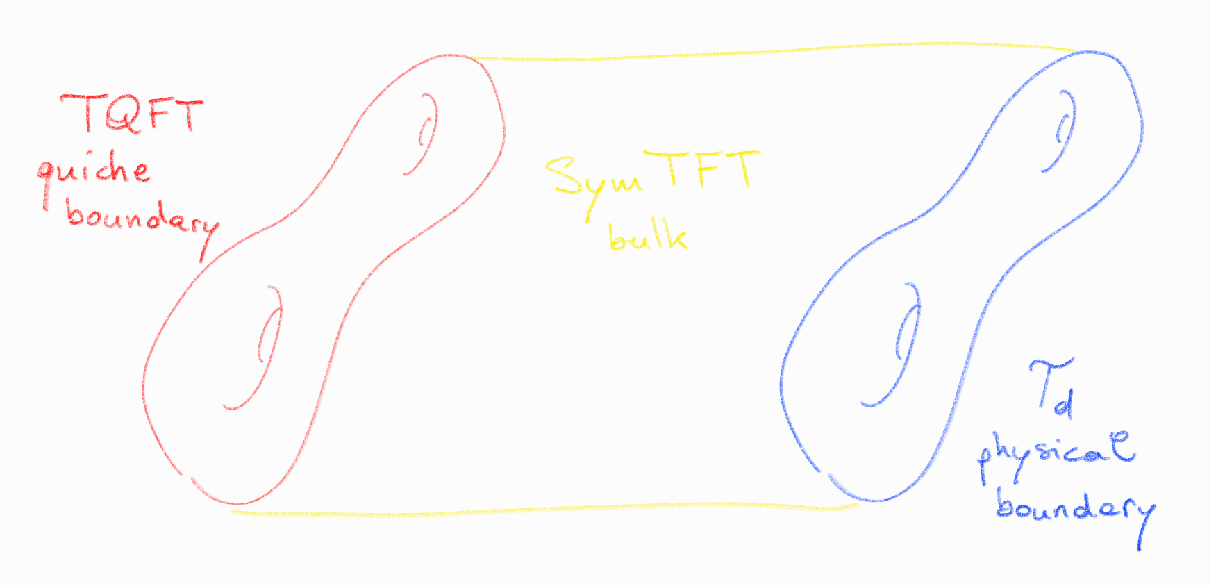
\includegraphics[width=0.75\linewidth]{images/13 sandwich_260702_171321.pdf}
    \caption{The sandwich construction.}
    \label{fig:sandwich}
\end{figure}

\begin{tcolorbox}
{\bf General Idea of the SymTFT}

The core philosophy of the SymTFT is to isolate the abstract symmetry data of a $d$-dimensional QFT $\mathcal{T}_d$ from its local dynamical degrees of freedom. This is achieved by declaring $\mathcal{T}_d$ to live on the $d$-dimensional boundary of a $(d+1)$-dimensional topological field theory, where the extra dimension is parametrized by a topologically trivial interval $t \in [0,1]$. Look at FIG. \ref{fig:sandwich}.

The physical $\text{QFT}_d$ is placed at the boundary $t=0$. At the opposite end of the interval ($t=1$), we impose a topological (gapped) boundary condition, commonly referred to as the \textit{quiche boundary}. Because the bulk theory is topological, the interval can be collapsed ($t \to 0$), sandwiching the two boundaries together. This projection completely defines the topological symmetry sector of the physical QFT, encoding all topological manipulations in terms of the chosen quiche boundary state.
\end{tcolorbox} 

To illustrate this construction formally, consider a $d$-dimensional QFT with a $\mathbb{Z}_N^{(p-1)}$ $(p-1)$-form global symmetry on $\mathcal{M}_d$. The corresponding $(d+1)$-dimensional SymTFT on $\mathcal{Y}_{D+1} = \mathcal{M}_d \times [0,1]$ can be formulated as a $BF$ theory of standard $U(1)$ gauge fields using the bulk action:
\begin{equation}\label{eq:zn_symtft_action}
    S_{\text{SymTFT}} = \frac{iN}{2\pi} \int_{\mathcal{Y}_{D+1}} B^{(D-p)} \wedge dA^{(p)}
\end{equation}
The gauge fields are not globally-defined differential forms: they are patched using standard $U(1)$ gauge transformations $\delta A^{(p)} = d\lambda^{(p-1)}$ and $\delta B^{(D-p)} = d\lambda^{(d-p-1)}$, which enforces the Dirac quantization conditions over any closed cycles:
\begin{equation}
    \frac{1}{2\pi} \int_{\gamma_{p+1}} dA^{(p)} \in \mathbb{Z} , \qquad \frac{1}{2\pi} \int_{\gamma_{d-p+1}} dB^{(D-p)} \in \mathbb{Z}
\end{equation}
The extended gauge-invariant operators in the bulk are Wilson lines and surfaces parameterized by continuous angles $\alpha, \beta \in \mathbb{R}$:
\begin{equation}
    U_\alpha(\gamma_{d-p}) = \exp\left(i\alpha \int_{\gamma_{d-p}} B^{(D-p)}\right), \qquad W_\beta(\gamma_p) = \exp\left(i\beta \int_{\gamma_p} A^{(p)}\right)
\end{equation}
Invariance under large gauge transformations requires $\alpha, \beta \in \mathbb{Z}$. Variations with respect to the field fluctuations give the bulk equations of motion $dA^{(p)} = 0$ and $dB^{(D-p)} = 0$, ensuring that these operators are strictly topological. Furthermore, summing over non-trivial $U(1)$ bundles in the path integral enforces the holonomies to be quantized:
\begin{equation}
    \frac{N}{2\pi}\int_{\gamma_p} A^{(p)} \in \mathbb{Z}, \qquad \frac{N}{2\pi}\int_{\gamma_{d-p}} B^{(D-p)} \in \mathbb{Z}
\end{equation}
This identification implies that shifting the charges by $N$ results in equivalent operators (e.g., $U_{\alpha} \sim U_{\alpha+N}$). The theory therefore contains a finite set of non-equivalent topological bulk operators $U_n$ and $W_m$ with $n,m \in \mathbb{Z}_N$. Their mutual braiding relation is determined by their bulk linking number:
\begin{equation}
    \langle U_n(\gamma_{d-p}) W_m(\gamma_p) \rangle = \exp\left(\frac{2\pi i mn}{N} \text{Link}(\gamma_{d-p}, \gamma_p)\right)
\end{equation}

With these two sets of topological operators, in absence of anomalies, we can decide which one we want to act as the charged objects (we make it terminate on the boundary, and the end-surface results into the charged operator in our physical QFT - it results in a one-dimension-less operator) and which one act as a symmetry operator (since we let the conjugate end on the boundary, we are not allowed to do the same with this, the operator can lay on the boundary without ending - resulting in a topological operator of the same dimension in the physical QFT).

\subsubsection{A complementary perspective: Hamiltonian Formulation and Choice of Boundary Conditions}

A physically intuitive perspective emerges if we align the coordinate time of the Euclidean $(d+1)$-dimensional bulk with the direction of the interval $t \in [0,1]$. When computing correlation functions, the path integral can be interpreted as an overlap in the bulk Hilbert space $\mathcal{H}[\mathcal{M}_d]$ between the physical boundary state at $t=0$ and the quiche boundary state at $t=1$. 

\begin{tcolorbox}
    {\bf Canonical picture vs Path Integral}

    Remember that whenever we define a Path integral on a manifold with boundary, it defines naturally an Hilbert space on the boundary, and the boundary condition we need to perform the path integral corresponds to the state in the Hilbert space.

    When we have two boundaries\footnote{For example when we are considering $\mathcal{M}_{d} = \Sigma_{d-1}\times I$, we have the boundary in the past and the one in the future.}, we need two boundary conditions or states in the Hilbert spaces. What the Path Integral does when we we compute it using these boudnary condition is the amplitude given by the overlap of these states.
\end{tcolorbox}

Since $A^{(p)}$ and $B^{(D-p)}$ are canonically conjugate variables, the bulk Hilbert space admits two dual, orthonormal bases of boundary states. A specific choice of boundary condition corresponds to choosing a maximal set of mutually-transparent bulk operators—known as a \textit{Lagrangian algebra} $\mathcal{L}$—that can end on the boundary, setting them to trivial values there.
\begin{enumerate}[\itshape i)]
    \item \textbf{Dirichlet Boundary Condition:} The Dirichlet state $|A\rangle$ diagonalizes the $A^{(p)}$ operators, fixing the classical background field $A$ for the global symmetry on the boundary:
    \begin{equation}
        W_m(\gamma_p)|A\rangle = e^{im \oint_{\gamma_p} A} |A\rangle
    \end{equation}
    The operators $W_m \in \mathcal{L}$ can terminate on the boundary, and their endpoints correspond to charged operators. Conversely, the dual operators $U_n$ cannot terminate and must lie flat on the boundary, acting as the topological symmetry defects of a boundary $\mathbb{Z}_N^{(p-1)}$ $(p-1)$-form symmetry. Intersecting the boundary QFT state yields the ungauged partition function: $\langle \text{QFT}|A\rangle = \mathcal{Z}_{\mathcal{T}}[A]$.
    
    \item \textbf{Neumann Boundary Condition:} The Neumann state $|N_B\rangle$ diagonalizes the $B^{(D-p)}$ operators, setting $U_n \in \mathcal{L}$:
    \begin{equation}
        U_n(\gamma_{d-p})|N_B\rangle = e^{in \oint_{\gamma_{d-p}} B} |N_B\rangle
    \end{equation}
    Here, the defects $U_n$ terminate on the boundary, leaving their duals $W_m$ to lie flat on it, which realizes a dual $\mathbb{Z}_N^{(d-p-1)}$ $(d-p-1)$-form symmetry. The Dirichlet and Neumann states are related by a discrete Fourier transform describing the condensation of the defects:
    \begin{equation}
        |N_B\rangle = \frac{1}{\sqrt{|H^p(\mathcal{M}_d, \mathbb{Z}_N)|}} \sum_{A} \exp\left(\frac{iN}{2\pi} \int_{\mathcal{M}_d} A \wedge B\right) |A\rangle
    \end{equation}
    Projecting the QFT state onto this boundary yields the flat-gauged partition function: $\langle \text{QFT}|N_B\rangle = \mathcal{Z}_{\mathcal{T}/\mathbb{Z}_N}[B]$.
\end{enumerate}

\subsubsection{'t Hooft Anomalies in the Discrete SymTFT}

{\bf 't Hooft anomalies are incorporated into the SymTFT by adding classical topological terms to the bulk action written in terms of the background fields.} 

Consider a $4d$ boundary theory with a $\mathbb{Z}_N^{(0)}$ symmetry; a pure anomaly is represented by a $5d$ Chern-Simons term added to the bulk action:
\begin{equation}\label{eq:anomalous_symtft_action}
    S_{\text{SymTFT}} = \frac{iN}{2\pi} \int_{\mathcal{Y}_5} dB^{(3)} \wedge A^{(1)} + \frac{i\kappa}{24\pi^2} \int_{\mathcal{Y}_5} A^{(1)} \wedge dA^{(1)} \wedge dA^{(1)}
\end{equation}
This term shifts the bulk equations of motion to 
\begin{equation}
    dA^{(1)} = 0 \qquad \& \qquad \frac{N}{2\pi} dB^{(3)} + \frac{\kappa}{8\pi^2} dA^{(1)} \wedge dA^{(1)} = 0
\end{equation}

{\bf The fact that $B^{(3)}$ is no longer closed in the presence of background curvature implies that the $U_n$ operators pick up a non-trivial phase under self-intersections, which prevents their condensation and completely obstructs the existence of a well-defined Neumann boundary state $|N_B\rangle$. }

Evaluating the classical variation of \eqref{eq:anomalous_symtft_action} at the boundary yields:
\begin{equation}
    \delta S_{\text{SymTFT}} = \frac{iN}{2\pi} \int_{\mathcal{M}_4} \delta A^{(1)} \wedge \left( B^{(3)} + \frac{i\kappa}{6\pi N} A^{(1)} \wedge dA^{(1)} \right) = 0
\end{equation}
which demands either $\delta A^{(1)}\big|_{\mathcal{M}_4} = 0$ (the consistent Dirichlet choice) or $\left. B^{(3)} + \frac{2\pi\kappa}{3N(4\pi^2)} A^{(1)} \wedge dA^{(1)} \right|_{\mathcal{M}_4} = 0$. The latter attempted Neumann condition is explicitly incompatible with the bulk equations of motion and fails to form a valid Lagrangian subspace.

{\bf We have seen that given a $\mathbb{Z}^{(0)}_N$ with a pure 't Hooft anomaly, we can have our symmetry structure representing the Dirichlet BC, allowing us to compute the partition function of the ungauged theory: $\mathcal{Z}_\mathcal{T}[A] = \langle QFT | A \rangle$. But, we are not allowed to gauge the symmetry and define the Neumann BC, as we expect from the presence of an anomaly.}

%---------------------------------------------------------
\subsection{Continuous $U(1)$ Symmetries via $\mathbb{R}$ and $U(1)$ Bulk Gauge Fields}
\label{sec:symtft_continuous_gauging}
%---------------------------------------------------------

To describe continuous $U(1)$ symmetries without introducing artificial periodicities in the symmetry parameters, we must alter the nature of the bulk gauge fields. Following \cite{Antinucci_2025}, continuous symmetries can be captured by choosing different combinations of $\mathbb{R}$-valued fields (which are globally-defined forms subject only to small gauge transformations) and $U(1)$-valued fields.

\subsubsection{The $\mathbb{R} \times \mathbb{R}$ SymTFT Formulation}
\label{sec:R_R_symtft}

We first analyze the case where both fields in the bulk are $\mathbb{R}$-gauge fields, denoted by lowercase letters $a^{(p)}$ and $b^{(D-p)}$. The bulk action is:
\begin{equation}
    S_{\mathbb{R}\times\mathbb{R}} = \frac{i}{2\pi} \int_{\mathcal{Y}_{D+1}} b^{(D-p)} \wedge da^{(p)}
\end{equation}
Since $\mathbb{R}$-bundles are topologically trivial, the Dirac quantization conditions collapse by Stokes' theorem, meaning $da^{(p)} = 0$ and $db^{(D-p)} = 0$ identically in the bulk. There are no large gauge transformations,\footnote{Gauge transformations are maps from our base space to the gauge group $\Lambda : \mathcal{M} \to \mathcal{G}$, the trivial map it the constant map into the identity element of the group. Large gauge transformations are the ones that cannot be continuously deformed into the trivial map. For $\mathcal{G}=U(1)$ there are many, but for $\mathcal{G}=\mathbb{R}$ there are none.} so the extended topological operators:
\begin{equation}
    U_\alpha (\gamma_{d-p}) = \exp \left(i\alpha \int_{\gamma_{d-p}} b^{(D-p)}\right) \qquad \& \qquad W_\beta (\gamma_p) = \exp \left(i\beta \int_{\gamma_p} a^{(p)}\right)
\end{equation}
are fully gauge-invariant for any arbitrary real coefficients $\alpha, \beta \in \mathbb{R}$. 

Imposing a boundary condition where all $W_\beta$ operators terminate on $\mathcal{M}_d$, i.e. $W_\beta \subset \mathcal{L}$, allows for generic real charges $\beta \in \mathbb{R}$, leaving the $U_\alpha$ operators lay without ending on the boundary to generate an $\mathbb{R}^{(p-1)}$ $(p-1)$-form symmetry (an example being a free non-compact scalar for $p=1$). Dually in a topological way, letting all $U_\alpha$ terminate corresponds to an $\mathbb{R}^{(d-p-1)}$ symmetry, which physically describes the flat gauging of the entire continuous $\mathbb{R}$ symmetry group on the boundary.

A generalized Maxwell theory (such as a compact scalar field, a free photon or a free $2$-form photon) is engineered by choosing a Lagrangian algebra where only the discrete subset of operators $U_n$ and $W_m$ with $n,m \in \mathbb{Z}$ can terminate on the boundary. The remaining non-equivalent bulk operators that can reside on the boundary are labeled by the coset classes $\alpha, \beta \in \mathbb{R}/\mathbb{Z} \cong U(1)$. This choice yields a boundary theory with an ordinary $U(1)^{(p-1)} \times U(1)^{(d-p-1)}$ global symmetry structure. 

It might seem that we are missing the mixed anomaly between these two symmetries, but we are not. Look at the discussion around EQ. \ref{eq:maxwell_sytft_u1}.

\subsubsection{The $U(1) \times \mathbb{R}$ SymTFT Formulation}
\label{sec:U1_R_symtft}

An alternative formulation that isolates a single continuous $U(1)$ symmetry is constructed by pairing a $U(1)$ gauge field $A^{(p)}$ with an $\mathbb{R}$ gauge field $b^{(D-p)}$ \cite{Antinucci_2025, Antinucci:2024bny}:
\begin{equation}\label{eq:u1_r_action}
    S_{U(1)\times\mathbb{R}} = \frac{i}{2\pi} \int_{\mathcal{Y}_{D+1}} b^{(D-p)} \wedge dA^{(p)}
\end{equation}
The Dirac quantization constraints for this mixed system read $\frac{1}{2\pi}\int dA^{(p)} \in \mathbb{Z}$ and $db^{(D-p)} = 0$. Due to the large gauge transformations of $A^{(p)}$, the allowed spectrum of bulk topological operators becomes asymmetric: 
\begin{equation}
    U_\alpha(\gamma_{d-p}) \quad \text{with} \quad \alpha \in \mathbb{R}/\mathbb{Z} \cong U(1) \qquad \& \qquad W_m(\gamma_p) \quad \text{with} \quad m \in \mathbb{Z}
\end{equation}
This formulation naturally hosts two distinct gapped boundary conditions:
\begin{enumerate}[\itshape i)]
    \item \textbf{Continuous $U(1)$ Symmetries:} Letting the discrete defects $W_m$ ($m \in \mathbb{Z}$) terminate on the boundary implies ($W_m \subset \mathcal{L}$) that the boundary charged operators carry integer charges. The continuous operators $U_\alpha$ ($\alpha \in U(1)$) are restricted to lie flat on the boundary, generating a continuous $U(1)^{(p-1)}$ global symmetry.
    \item \textbf{Discrete $\mathbb{Z}$ Symmetries:} Letting all continuous operators $U_\alpha$ ($\alpha \in U(1)$) terminate on the boundary ($U_\alpha \subset \mathcal{L}$) corresponds to a flat gauging of the entire $U(1)$ group on the boundary. This leaves the discrete operators $W_m$ ($m \in \mathbb{Z}$) flat on the boundary, defining a discrete $\mathbb{Z}^{(d-p-1)}$ $(d-p-1)$-form global symmetry.
\end{enumerate}

\subsubsection{Dynamical Gauging and Continuous SymTFT Maps}
\label{sec:dynamical_gauging_symtft}

A fundamental divergence between discrete and continuous global symmetries lies in the geometric nature of their gauging operations. For a discrete symmetry, performing a global manipulation corresponds strictly to a topological choice of boundary conditions (Dirichlet vs. Neumann) within a \textbf{single, unique} bulk SymTFT. Conversely, the dynamical gauging of a continuous $U(1)$ symmetry—such as coupling a matter current to a dynamical photon—is fundamentally a non-topological manipulation that alters the localized boundary DOF. In the bulk framework, such dynamical manipulations are implemented not by sweeping through boundary conditions of the same theory, but rather by an explicit, controlled map between two \textbf{distinct} SymTFTs \cite{Antinucci_2025, Antinucci:2024bny}.\footnote{This is different from the proposal of \cite{brennan2024symtftcontinuoussymmetries} which essentially treats dynamical gauging as a sum over boundary conditions.}

To contextualize this mechanism, consider a $d$-dimensional free complex scalar field possessing a continuous $U(1)^{(0)}$ $0$-form symmetry. Its associated $(d+1)$-dimensional SymTFT is described by a single $U(1) \times \mathbb{R}$ mixed BF action with $p=1$:
\begin{equation}\label{eq:matter_symtft}
    S_{\text{matter}} = \frac{i}{2\pi} \int_{\mathcal{Y}_{D+1}} b^{(d-1)} \wedge dA^{(1)}
\end{equation}
Dynamically gauging this symmetry promotes $A^{(1)}$ to a fluctuating connection, flowing the boundary system to scalar Quantum Electrodynamics (QED). The dual system now inherently features a magnetic $U(1)^{(d-3)}$ $(d-3)$-form global symmetry, whose bulk SymTFT presentation shifts the form degrees to $p=2$:
\begin{equation}\label{eq:qed_symtft}
    S_{\text{QED}} = \frac{i}{2\pi} \int_{\mathcal{Y}_{D+1}} f^{(2)} \wedge dF^{(d-2)}
\end{equation}
The map connecting \eqref{eq:matter_symtft} to \eqref{eq:qed_symtft} is fully determined in the bulk by adding the SymTFT of a pure $d$-dimensional photon and implementing a linking coupling that forces the localized topological operators to match the boundary physics, as discussed in \cite{Antinucci_2025, Antinucci:2024bny}. 

\begin{tcolorbox}
{\bf Derivation of the Continuous Gauging Map, through an example}

We model the dynamical $1$-form photon sector through its alternative three-field formulation made by two $U(1)$ gauge fields with a mixed anomaly -as in \ref{sec:U1_R_symtft}- rather that two $\mathbb{R}$ gauge fields -as in \ref{sec:R_R_symtft}- \cite{Antinucci_2025, Antinucci:2024bny}:\footnote{Using the EOM it can be recast into a SymTFT of two $\mathbb{R}$ gauge fields as in \ref{sec:R_R_symtft}.}
\begin{equation}\label{eq:maxwell_sytft_u1}
    S_{\text{photon}} = \frac{i}{2\pi} \int_{\mathcal{Y}_{D+1}} \left( g^{(d-2)} \wedge dG^{(2)} + f^{(2)} \wedge dF^{(d-2)} - G^{(2)} \wedge dF^{(d-2)} \right)
\end{equation}
To implement the physical minimal coupling on the boundary—where the Wilson lines of the Maxwell field can end on the charged matter operators—we must allow the bulk surfaces of $G^{(2)}$ to terminate directly on the lines of $A^{(1)}$. We stitch the two sectors together via the bulk coupling $b^{(d-1)} \wedge G^{(2)}$:
\begin{multline}
\label{eq:total_gauged_action}
    S_{\text{total}} = \frac{i}{2\pi} \int_{\mathcal{Y}_{D+1}}  b^{(d-1)} \wedge dA^{(1)} + b^{(d-1)} \wedge G^{(2)} + g^{(d-2)} \wedge dG^{(2)} + \\ 
    + f^{(2)} \wedge dF^{(d-2)} - G^{(2)} \wedge dF^{(d-2)} 
\end{multline}
The presence of the non-derivative linking term forces a modification of the standard gauge transformations, setting $\delta G^{(2)} = d\lambda^{(1)}$ and $\delta A^{(1)} = -\lambda^{(1)}$. Consequently, the isolated lines of $A^{(1)}$ are no longer gauge invariant, but form non-genuine\footnote{Genuine and non-genuine is a concept we introduced in \ref{sec:genuine_op}.} open operators attached to a bounding disk:
\begin{equation}
    L_n(\gamma_1, \mathcal{D}_2) = \exp \left( in\int_{\gamma_1} A^{(1)} + in\int_{\mathcal{D}_2} G^{(2)} \right), \qquad \partial\mathcal{D}_2 = \gamma_1
\end{equation}
Dually, the gauge variation of $b^{(d-1)}$ acts on $g^{(d-2)}$ as $\delta b^{(d-1)} = d\eta^{(d-2)}$ and $\delta g^{(d-2)} = (-1)^{d}\eta^{(d-2)}$, which trivializes and breaks the continuous $U(1)^{(0)}$ symmetry defects. Integrating out the trivialized topological sectors leaves \eqref{eq:total_gauged_action} exactly equivalent to the dual QED SymTFT \eqref{eq:qed_symtft}. This non-topological transition corresponds algebraically to the formal substitution map:
\begin{equation}\label{eq:symtft_gauging_map}
    dA^{(1)} \longrightarrow f^{(2)} \qquad \& \qquad b^{(d-1)} \longrightarrow dF^{(d-2)}
\end{equation}
\end{tcolorbox}

The first substitution in \eqref{eq:symtft_gauging_map} dictates that $A^{(1)}$, which was constrained to be a flat classical background connection in the original SymTFT, is mapped to a unconstrained, dynamic curvature field strength $f^{(2)}$ at the boundary. The second substitution tracks the trivialization of the original global current in terms of a lower-degree magnetic form.

\paragraph*{Generalization:} This is how we motivate the proposal appeared in \cite{Antinucci_2025} that the dynamical gauging of a $U(1)^{(p)}$ symmetry in the physical QFT theory can be understood from the SymTFT POV as starting from the bulk theory
\begin{equation}
    \mathcal{S}_{SymTFT} = \frac{i}{2\pi} \int_{\mathcal{Y}_{D+1}} b^{(d-p-1)} \wedge dA^{(p+1)} + (\text{anomaly terms containing $b,A$})
\end{equation}
and performing the substitutions
\begin{equation}
    b^{(d-p-1)} \to dF^{(d-p-2)} \qquad \& \qquad dA^{(p+1)} \to f^{(p+2)}
\end{equation}
obtaining the SymTFT of a $U(1)^{(d-p-3)}$ symmetry. Notice this is in accordance with what we expect from dynamical gauging, as discussed in \ref{sec:gauging_and_dual}.

\begin{tcolorbox}
{\bf The Anomaly Polynomial TFT}

To unify these distinct, continuous SymTFTs into a single framework, one can construct a unique $(d+2)$-dimensional TQFT whose $(d+1)$-dimensional topological boundaries correspond to the alternate theories related by dynamical manipulations \cite{Antinucci_2025}. 

For a $4d$ theory with a $U(1)^{(0)}$ symmetry and a pure anomaly $\kappa$, this \textit{Anomaly Polynomial TFT} takes the form on $\mathcal{X}_6$:
\begin{equation}
    S_{\text{AnomPolyTFT}} = \frac{i}{2\pi} \int_{\mathcal{X}_6} \left( g^{(3)} \wedge df^{(2)} - \frac{\kappa}{12\pi} f^{(2)} \wedge f^{(2)} \wedge f^{(2)} \right)
\end{equation}
Where $g,f$ are $\mathbb{R}$ gauge fields and in the boundary theory (the SymTFT) they are coupled as conjugate variables to the $U(1)$ gauge fields.

When $\kappa = 0$, this bulk structure admits two valid boundary conditions yielding the ungauged matter SymTFT or the gauged QED SymTFT, which are mapped into each other via \eqref{eq:symtft_gauging_map}. When $\kappa \neq 0$, the gauge variation along the boundary cannot be cancelled if the $U(1)$ symmetry is gauged, leaving the QED boundary sector anomalous and geometrically inconsistent. 
\end{tcolorbox}

\newpage
%---------------------------------------------------------
\section{Laboratory:}
%---------------------------------------------------------

%---------------------------------------------------------
\subsection{Free Fermion and ABJ Anomaly in $4d$: Non-Invertible Symmetries}
\label{sec:abj_example}
%---------------------------------------------------------

Consider the theory of a single massless $4d$ Dirac fermion $\Psi$. Classically, the system exhibits an ordinary $0$-form global symmetry group $G = U(1)^{(0)}_V \times U(1)^{(0)}_A$, corresponding to vector and axial transformations acting on the fields as $\Psi \to e^{i\beta} \Psi$ and $\Psi \to e^{i\alpha \gamma_5} \Psi$, respectively. 

The physical theory is defined by the standard Lagrangian action coupled to classical background connections:
\begin{equation}
    S = \int_{\mathcal{M}_4} i \bar{\Psi} \gamma^\mu \left( \partial_\mu - i B_\mu^{(1),V} - i B_\mu^{(1),A} \gamma_5 \right) \Psi \star 1
\end{equation}
The total anomaly structure of this un-gauged, free theory is captured by the $6$-form anomaly polynomial $\mathcal{I}_6$:
\begin{equation}
    \mathcal{I}_6 = \frac{1}{4 \pi^2} F_A \wedge F_V \wedge F_V + \frac{1}{12 \pi^2} F_A \wedge F_A \wedge F_A
\end{equation}
where $F_V = dB^{(1)}_V$ and $F_A = dB^{(1)}_A$ are the field strengths of the classical background gauge fields for $U(1)_V$ and $U(1)_A$. 

\subsubsection{The Bulk Symmetry TFT Description}

To unearth the topological structure of these symmetries, we lift the system to a $5d$ SymTFT defined on $\mathcal{Y}_5$. The uncompactified bulk theory contains two copies of $1$-form $U(1)$ BF theories, where the $1$-form fields $B^{(1)}_A$ and $B^{(1)}_V$ represent the extensions of the boundary backgrounds, while $b^{(3)} $ and $c^{(3)} $ act as their conjugate top-form multipliers. 

The mixed $U(1)_A \times U(1)_V^2$ triangle anomaly and the pure $U(1)_A^3$ anomaly are implemented via bulk Chern-Simons terms:
\begin{multline}
\label{eq:SymTFT_ungauged}
    \mathcal{S}_{\text{SymTFT}} =  \frac{i}{2\pi} \int_{\mathcal{Y}_5}  b^{(3)} \wedge dB^{(1)}_A + c^{(3)}  \wedge dB^{(1)}_V + \\ + \frac{l}{4\pi} B^{(1)}_A \wedge dB^{(1)}_V \wedge dB^{(1)}_V  + \frac{k}{12\pi} B^{(1)}_A \wedge dB^{(1)}_A \wedge dB^{(1)}_A
\end{multline}
For a single $4d$ Dirac fermion, the exact anomaly coefficients are $l = 2$ and $k = 2$. 

The mixed anomaly term $B^{(1)}_A \wedge dB^{(1)}_V \wedge dB^{(1)}_V$ introduces an immediate obstruction in the quiche state space: it is impossible to impose simultaneous Neumann boundary conditions for both $B^{(1)}_A$ and $B^{(1)}_V$, meaning that $U(1)_V$ and $U(1)_A$ cannot be gauged dynamically at the same time.

\subsubsection{Dynamical Gauging of $U(1)_V$ and the Non-Invertible Defect}

We now perform a dynamic gauging of the vector symmetry $U(1)_V$ to flow to Quantum Electrodynamics (QED). In the SymTFT language, following the prescription detailed in \ref{sec:dynamical_gauging_symtft}, this non-topological manipulation translates to the mapping substitutions:
\begin{equation}
    dB^{(1)}_V  \longrightarrow   f^{(2)} \qquad \text{and} \qquad c^{(3)} \longrightarrow dG^{(2)}
\end{equation}
transforming the vector background into a dynamic bulk field strength $f^{(2)}$ and its dual multiplier into a $2$-form gauge connection $G^{(2)}$. This yields the new bulk SymTFT for the dynamically gauged QED-like boundary theory:
\begin{multline}\label{eq:SymTFT_QED}
    S_{\text{SymTFT}}^{\text{QED}} = \frac{i}{2\pi} \int_{\mathcal{Y}_5}  b^{(3)} \wedge dB^{(1)}_A + f^{(2)} \wedge dG^{(2)} +\\+ \frac{2}{4\pi} B^{(1)}_A \wedge f^{(2)} \wedge f^{(2)} + \frac{2}{12\pi} B^{(1)}_A \wedge dB^{(1)}_A \wedge dB^{(1)}_A 
\end{multline}
Because of the non-derivative cubic coupling $B^{(1)}_A \wedge f^{(2)} \wedge f^{(2)}$, the classical bulk fields must be patched using modified gauge transformations to ensure the invariance of the action. Under the variations $\delta B^{(1)}_A = d\rho^{(0)}$ and $\delta f^{(2)} = d\lambda^{(1)}$, the fields $b^{(3)}$ and $G^{(2)}$ transform non-trivially as:
\begin{equation}\label{eq:gauge_trans_qed}
    \delta b^{(3)} = -\frac{2}{4\pi} \lambda^{(1)} \wedge d\lambda^{(1)} - \frac{2}{2\pi} \lambda^{(1)} \wedge f^{(2)}, \qquad \delta G^{(2)} = -\frac{2}{2\pi}\rho^{(0)}\left(f^{(2)} + d\lambda^{(1)}\right) - \frac{2}{2\pi}\lambda^{(1)} \wedge B^{(1)}_A
\end{equation}
Varying the action with respect to the continuous fluctuations gives the modified bulk equations of motion for the higher-form fields:
\begin{equation}\label{eq:ABJ_EOM}
    dG^{(2)} + \frac{1}{2\pi} dB^{(1)}_A \wedge f^{(2)} = 0, \qquad db^{(3)} + \frac{1}{2\pi} f^{(2)} \wedge f^{(2)} + \frac{1}{4\pi} dB^{(1)}_A \wedge dB^{(1)}_A = 0
\end{equation}
On the boundary $\mathcal{X}_4$, where the axial field $B^{(1)}_A$ is kept under flat Dirichlet conditions ($dB^{(1)}_A = 0$), the second equation reduces to $db^{(3)} = -\frac{1}{2\pi} f^{(2)} \wedge f^{(2)}$. This is the exact holographic manifestation of the Adler-Bell-Jackiw (ABJ) anomaly: the axial current is no longer conserved in the presence of dynamic electromagnetic field strengths, yielding $d \star j_A = \frac{1}{4\pi^2} f^{(2)} \wedge f^{(2)}$.

Consequently, the naive axial symmetry operator $U_\alpha(\mathcal{M}_3) = \exp(i\alpha \oint_{\mathcal{M}_3} b^{(3)} )$ is no longer topological. To restore its topological nature, we construct a non-genuine bulk operator $\widetilde{U}_\alpha(\mathcal{M}_3, \mathcal{D}_4)$ attached to an open $4d$ disk $\mathcal{D}_4$ such that $\partial \mathcal{D}_4 = \mathcal{M}_3$:
\begin{equation}
    \widetilde{U}_\alpha(\mathcal{M}_3, \mathcal{D}_4) = \exp\left(i\alpha \int_{\mathcal{M}_3} b^{(3)} + \frac{i\alpha}{2\pi} \int_{\mathcal{D}_4} f^{(2)} \wedge f^{(2)}\right)
\end{equation}
While $\widetilde{U}_\alpha$ is topological due to \eqref{eq:ABJ_EOM}, the explicit dependence on the bulk sheet $\mathcal{D}_4$ implies that for a generic continuous angle $\alpha$, the operator cannot reside genuinely on the boundary.

A consistent localization on $\mathcal{M}_3$ is achievable if $\alpha$ takes rational values, $\alpha = \frac{p}{2q}$ with $\gcd(p,q)=1$. For rational angles, the fractional bulk term can be compensated by the anomaly of a lower-dimensional fractional quantum Hall state localized on the defect. We define the minimal, genuine $3d$ topological symmetry operator by dressing the non-genuine defect with a minimal $3d$ $\mathbb{Z}_q$ TQFT, denoted as $\mathcal{A}_{q,p}[\mathcal{M}_3; f^{(2)}]$:
\begin{equation}\label{eq:non_inv_defect_def}
    D_{p/2q}(\mathcal{M}_3) = \widetilde{U}_{\alpha = \frac{p}{2q}}(\mathcal{M}_3) \times \mathcal{A}_{q,p}[\mathcal{M}_3; f^{(2)}]
   % \label{eq:dressed_axial_defect}
\end{equation}
where the $3d$ theory we used to decorate the original defect takes the form
\begin{equation}
    \mathcal{A}_{q,p}[\mathcal{M}_3; f^{(2)}] = \int \mathcal{D}c^{(1)} \exp\left( \frac{iqp}{4\pi}\int_{\mathcal{M}_3} c^{(1)} \wedge dc^{(1)} + \frac{ip}{2\pi}\int_{\mathcal{M}_3} c^{(1)} \wedge f^{(2)} \right)
\end{equation}

The internal $1$-form symmetry of the $3d$ TQFT $\mathcal{A}_{q,p}$ couples directly to the bulk dynamical electromagnetic field $f^{(2)}$. Under a gauge variation, the inflow from $\mathcal{A}_{q,p}$ precisely cancels the sheet-dependence of $\widetilde{U}_\alpha$, making $D_{p/2q}(\mathcal{M}_3)$ a well-defined, gauge-invariant, genuine topological defect.\footnote{This construction is similar to the anomaly inflow, but there are differences: the object of our interest is the one with an extra dimension, and the non invariance is WRT dynamical fields, not background.} 

Notice the theory we have used to decorate the defect has been borrowed from Condensed Matter Theory, where it is known as Fractional Quantum Hall state.

The presence of the internal $3d$ TQFT path integral within the definition of the operator alters its algebraic structure: the operator is no longer unitary and lacks a group-like inverse. When fused with its conjugate defect, it does not yield the identity but rather projects onto a condensation defect \cite{Roumpedakis_2023}. The continuous, invertible $U(1)_A$ axial symmetry has thus transmuted into a discrete, non-invertible $\mathbb{Q}/\mathbb{Z}$ generalized global symmetry.


\subsection{Complex scalar boson and Abelian-Higgs model in $3d$}
\label{sec:complex_boson_3d}

Within this section, we investigate the Renormalization Group (RG) evolution of generalized symmetries within the $3d$ $U(1)$ $XY$-model

\begin{equation}\label{eq:xy_model}
    \mathcal{S}_{XY}[\phi;m,\lambda] = \int_{\mathcal{M}_3}  d \phi \wedge \star d \bar \phi  + m^2 \phi \wedge \star \bar \phi + \frac{\lambda}{2}  |\phi|^4 \star 1
\end{equation}
Where we kept all the relevant terms.\footnote{In $3d$, the scaling dimension  is $[\phi] =  \frac{1}{2}$. Consequently, the operator $|\phi|^6$ has a classical dimension of $3$, rendering it strictly marginal in the UV. However, at the Infrared Wilson-Fisher (WF) fixed point, the anomalous dimension shifts the operator to $\Delta_{|\phi|^6} > 3$, making it strictly irrelevant. Then, considering only $|\phi|^2$ and $|\phi|^4$ is justified when defining the minimal Landau-Ginzburg action within the same universality class, as $|\phi|^6$ does not alter the IR critical behavior.} It has two phases: an unbroken/disordered phase (the system is gapped) for $m^2 > 0$ and a SSB/ordered phase (Superfluid \ref{eq:superfluid}) for $m^2 < 0$; in between there is a Wilson-Fisher fixed point, look at FIG. \ref{fig:rg_flow_xymodel}. This theory has two DOF in the UV, where it is weakly coupled.

\begin{figure}
    \centering
    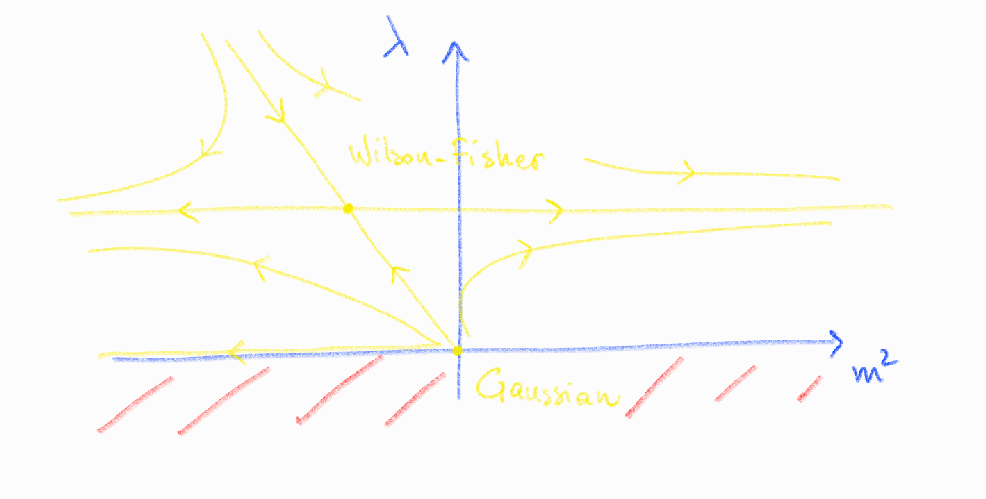
\includegraphics[width=0.75\linewidth]{images/14 rg xym9del_260702_171624.pdf}
    \caption{Renormalization group flow of $XY$-model in $4d$, but it is believed to be the same in $3d$.}
    \label{fig:rg_flow_xymodel}
\end{figure}

And its dual counterpart,\footnote{This IR duality (Peskin-Halperin-Dasgupta-Halperin duality) establishes the quantum equivalence between the $O(2)$ Wilson-Fisher fixed point and the critical regime of the Abelian-Higgs model, identifying the scalar field of one description with the topological vortex operators of the dual description.} the Abelian-Higgs model.
\begin{equation}
    \mathcal{S}_{AH}[f,\phi;e,m,\lambda] = \int  \frac{1}{2 e^2} f \wedge \star f + \mathcal{D} \phi \wedge \star \mathcal{D} \bar \phi + m^2 \phi \wedge  \star \bar \phi + \frac{\lambda}{2}  |\phi|^4  \star 1 
\end{equation}
This theory has two regimes (we allow $m^2 \in \mathbb{R}$, while $e^2 \in \mathbb{R}^+$ ): when $|m| \ll e^2$ the theory is strongly coupled in the IR (differently from Maxwell theory in $4d$, where the IR is a free theory), instead when $|m| \gg e^2$ the theory is weakly coupled.

{\bf Looking at $|m| \gg e^2$, we have to scenarios.}

\paragraph*{If $m^2$ is positive:} then to study the IR behaviour we can simply integrate out the scalar $\phi$. We obtain free Maxwell theory (gapless Coulomb phase). Here, the magnetic symmetry $U(1)^{(0)}_m$, $j^{(1)}_m \approx \star f$, is SSB and we have an emergent $U(1)^{(1)}_e$, $j^{(2)}_e \approx  f$, electric symmetry, since at this energy we don't have access to the charged DOF anymore. The two symmetries are bonded by a mixed anomaly, $\mathcal{I}_5 =  \frac{1}{4\pi^2} F^{(3)}_e \wedge F^{(2)}_m$.

\paragraph*{If $m^2$ is negative:} the scalar condenses at $\langle |\phi| \rangle^2 = -m^2/\lambda$, the Anderson-Higgs mechanism occurs, and we obtain the Higgs phase. This phase has a massive photon DOF, it is gapped, and has only the magnetic symmetry $U(1)^{(0)}_m$, $j^{(1)}_m \approx \star f$, being unbroken.

\begin{tcolorbox}
    {\bf Statistical mechanics point of view}

    If we reinterpret our Euclidean field theory from describing $2+1d$ QFT to $3+0d$ Statistical Field Theories, we realize that the $XY$-model is describing for example Superfluid transition of liquid Helium, while the Abelian-Higgs model is describing for example Superconductor transition.

    Furthermore, we realize that given the duality maps $m^2 \leftrightarrow -m^2$, and that in both cases $m^2$ probes the distance from the critical temperature $T_C$, i.e. corresponds to the reduced temperature $T-T_C$, we have a map between low temperature and high temperature. In particular, low temperature superconductors are governed by the same physics of high temperature superfluids, and viceversa.
\end{tcolorbox}


\subsubsection{The web of dualities}
The $3d$ $XY$ and Abelian-Higgs (AH) models each exhibit two distinct infrared (IR) regimes determined by their ultraviolet (UV) mass deformations. For the $XY$-model, parameterized by the mass squared $m_{XY}^2$, these comprise the gapless superfluid phase \ref{eq:superfluid}—characterized by the spontaneous symmetry breaking (SSB) of the global $U(1)^{(0)}$ phase rotation symmetry—and the trivially gapped unbroken scalar phase ($m_{XY}^2 \gg 0 $). Conversely, the AH model, parameterized by $m_{AH}^2$, features a gapless free-Maxwell Coulomb phase ($m_{AH}^2 \gg e^4$) and a topologically gapped superconductor (Higgs) phase ($m_{AH}^2 \ll -e^4$).

Particle-vortex duality establishes an IR equivalence between these theories under the parameter mapping $m_{AH}^2 \approx -m_{XY}^2$. This duality maps the XY superfluid to the AH Coulomb phase, and the unbroken scalar to the AH Higgs phase. At the operator level, the gapless superfluid phonon maps directly to the dual photon field via Hodge duality ($\star d\chi \sim f^{(2)}$), while the fundamental scalar field $\tilde{\phi}$ maps to the monopole disorder operator $\mathcal{M}(x) \sim e^{i\sigma (x)}$, thereby equating elementary particle excitations with topological vortices.

{\bf Dynamically gauging these global symmetries acts as an inter-theory map that permutes these regimes across the two systems.} Gauging the global $U(1)^{(0)}$ phase symmetry of the XY model yelds the AH model: gauging the superfluid phase triggers the standard cinematic Higgs mechanism, wherein the vector gauge field absorbs the Goldstone mode to acquire a mass, yielding the gapped Higgs phase. Gauging the unbroken scalar phase integrates out the heavy matter sector, leaving an un-screened, gapless AH Coulomb phase. Conversely, gauging the $U(1)^{(0)}_{m}$ magnetic current ($j^{(1)}_{m} = \frac{1}{2\pi}\star f^{(2)}$) of the AH model acts as the inverse map, projecting the Higgs phase back to the XY superfluid and the Coulomb phase to the unbroken scalar.

{\bf When closed under the complete particle-vortex duality web, the composition of gauging and dualization manifests as a stark intra-theory phase inversion that systematically exchanges gapped and gapless phases.} Look at FIG. \ref{fig:3d_web}. Gauging the global symmetry of either gapless phase (the XY superfluid or the AH Coulomb phase) drives the system into a trivially gapped IR vacuum. 

Conversely, gauging either gapped phase (the unbroken scalar or the Higgs phase) eliminates the mass gap and regenerates a gapless degree of freedom in the IR. 

\begin{figure}
    \centering
    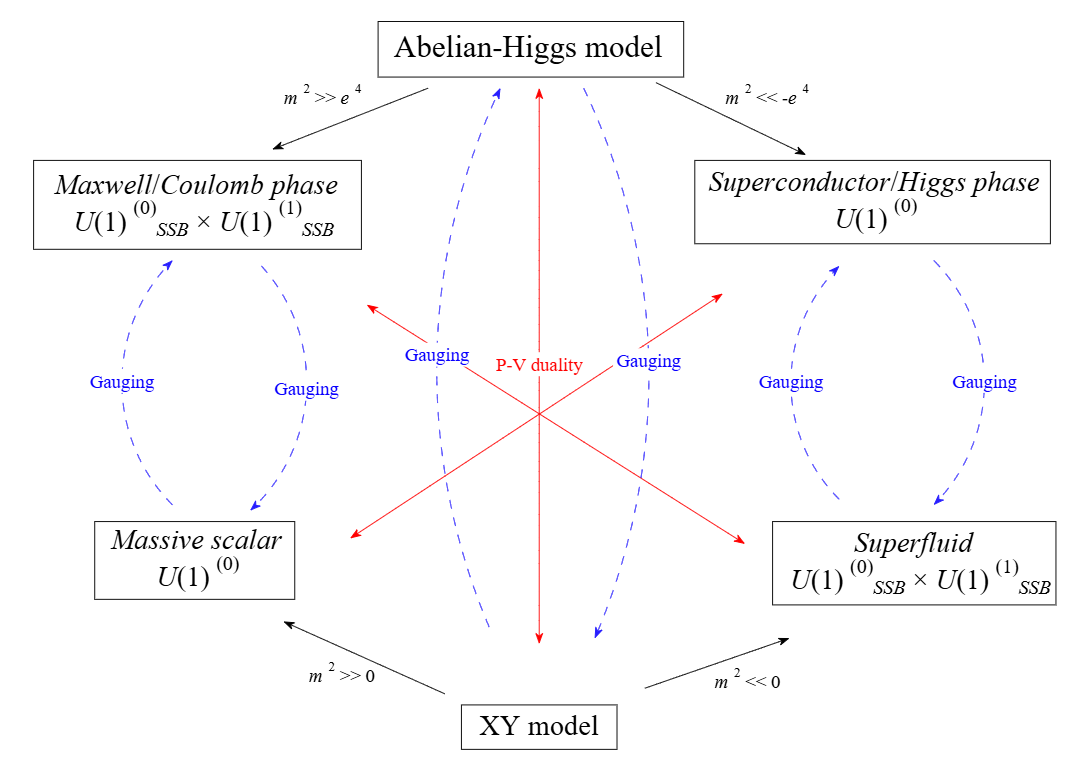
\includegraphics[width=0.75\linewidth]{images/duality_deb_3d.png}
    \caption{This is the map connecting the theories we have discussed. The solid red double-arrow lines represent particle vortex duality, the dashed blue single-arrow lines represent dynamical gauging of $U(1)^{(0)}$.}
    \label{fig:3d_web}
\end{figure}

%%%%%%%%%%%%%%%%%%%%%%%%%%%%%%%%%%%%%%%%%%%%%%%%%%%%%%%%%%%%%%%%%%%%%%%%
%%%%%%%%%%%%%%%%%%%%%%%%%  Maxwell Model  %%%%%%%%%%%%%%%%%%%%%%%%%%%%%%
%%%%%%%%%%%%%%%%%%%%%%%%%%%%%%%%%%%%%%%%%%%%%%%%%%%%%%%%%%%%%%%%%%%%%%%%

\subsection{Maxwell Model and its coupling with electric/magnetic charges}
\label{sec:gen_maxwell_couplings}

Consider a free Abelian $U(1)$ gauge theory defined on a smooth, compact $d$-dimensional Riemannian manifold $\mathcal{M}_d$ without boundary. The fundamental kinematic variable is the $1$-form connection $a^{(1)}$, which dictates the gauge-invariant $2$-form field strength $f^{(2)} = da^{(1)}$. The source-free Maxwell action is governed by the functional
\begin{equation}
\mathcal{S}[a^{(1)}] = \frac{1}{2e^2} \int_{\mathcal{M}_d} f^{(2)} \wedge \star f^{(2)},
\end{equation}
where $\star$ denotes the Hodge isomorphism and $e$ represents the gauge coupling constant. The classical dynamics and topology of the uncoupled field enforce two orthogonal conservation laws: the Euler-Lagrange equation $d\star f^{(2)} = 0$ and the geometric Bianchi identity $df^{(2)} = 0$.

These conservation conditions yield two distinct global topological symmetries, structured within the framework of generalized higher-form symmetries. The field equations protect a $1$-form electric symmetry $U(1)_e^{(1)}$, whose conserved $(d-2)$-form Noether current reads
\begin{equation}
j^{(2)}_e = \frac{1}{e^2} f^{(2)}, \quad d \star j_e = 0.
\end{equation}
Concurrently, the topology of the connection yields a $(d-3)$-form magnetic symmetry $U(1)_m^{(d-3)}$. Its associated $2$-form current is defined by
\begin{equation}
j^{(d-2)}_m = \frac{1}{2\pi} \star f^{(2)}, \quad d \star j_m = 0.
\end{equation}
The charged excitations under $U(1)_e^{(1)}$ and $U(1)_m^{(d-3)}$ correspond to non-local geometric operators, specifically $1$-dimensional Wilson lines $W(\mathcal{M}_1) = \exp(i \oint_{\mathcal{M}_1} a^{(1)})$ and $(d-3)$-dimensional 't Hooft operators $T(\mathcal{M}_{d-3})$, respectively.

This theory presents a mixed anomaly whose anomaly polynomial is 
\[
\mathcal{I}_{d+2} = \frac{1}{4\pi^2} F^{(3)}_e \wedge F^{(d-1)}_m
\]
where $F^{(3)}_e $ and $ F^{(d-1)}_m$ are the curvatures of the background fields WRT the $1$-form electric symmetry and the $(d-3)$-form magnetic symmetry, respectively.

\subsubsection{Dual Photon Formulation}
\label{subsec:dual_photon}

The independent physical degrees of freedom admit an equivalent description through Hodge dualization. By relaxing the closure constraint $df^{(2)} = 0$ in the path integral and introducing a $(d-3)$-form dual connection $\tilde{a}_{d-3}$ as a Lagrange multiplier to enforce it, one derives the dual field strength $g^{(d-2)} = d\tilde{a}_{d-3}$. The on-shell map between formulations is established by the duality relation
\begin{equation}
g^{(d-2)} = \star f^{(2)}.
\end{equation}
In terms of this dual photon variable, the free theory is recast via the dual action
\begin{equation}
S_{\text{dual}}[\tilde{a}_{d-3}] = \frac{e^2}{2} \int_{\mathcal{M}_d} g^{(d-2)} \wedge \star g^{(d-2)}.
\end{equation}
Under this transformation, the operational roles of the field equations and the Bianchi identities are interchanged. The equation of motion for $\tilde{a}_{d-3}$ recovers the original magnetic symmetry conservation, $dg^{(d-2)}=0$, while the Bianchi identity for $g^{(d-2)}$ maps to the electric current conservation.

{\bf This isomorphism between the two theories is called electro-magnetic (or Montonen–Olive, or S-) duality.}

\subsubsection{Explicit Symmetry Breaking via Matter Coupling}
\label{subsec:matter_coupling}

{\bf We now want to provide two theories, one with a $1$-form symmetry and the other one with a $d-3$-form symmetry.}

The introduction of dynamical matter sources explicitly breaks these generalized global symmetries by destroying the conservation of the respective currents. The specific choice of formulation dictates the nature of the minimal coupling.

In the standard representation, coupling the gauge field to an electrically charged scalar field $\phi$ with conservation current $J_e^{(1)}$, yields the Abelian-Higgs model \cite{Heidenreich_2021}. The inclusion of the dynamic matter current $J_e^{(1)}$ deforms the Maxwell equation: 
\begin{equation}
d\star f^{(2)} = e^2 \star J_e^{(1)}
\end{equation}
Consequently, $d \star j^{(2)}_e \neq 0$, which implies that the $1$-form electric symmetry $U(1)_e^{(1)}$ is explicitly broken. Wilson lines can now terminate on local scalar operators, reflecting the screening of electric charges. Crucially, because the underlying geometry $f^{(2)} = da^{(1)}$ is unperturbed, the Bianchi identity $df^{(2)} = 0$ remains satisfied, keeping the $(d-3)$-form magnetic symmetry $U(1)_m^{(d-3)}$ intact.\footnote{More generally, if we couple an electrically charged field with non-unit charge $q_e \in \mathbb{N}$, the symmetry group $U(1)^{(1)}_e$ breaks into $\mathbb{Z}_{q_e}$. This because, in this scenario some Wilson lines cannot be screened by charged operators, and thus they survive the coupling \cite{Heidenreich_2021, bhardwaj2023lecturesgeneralizedsymmetries}.}

Conversely, coupling the system to magnetically charged matter requires utilizing the dual photon formulation. We will call the obtained theory: Magnetic Abelian-Higgs model. 
Introducing a localized magnetic monopole current $J_m^{(d-3)}$ alters the dual field equations to 
\begin{equation}
d \star g^{(d-2)} = \frac{1}{e^2} \star J_m^{(d-3)} \implies df^{(2)} = \frac{1}{e^2} \star J_m^{(d-3)}
\end{equation}
This dynamic source explicitly breaks the $(d-3)$-form magnetic symmetry, as $d \star j^{(d-3)}_m \neq 0$, rendering the 't Hooft operators non-topological. In this configuration, the electric $1$-form symmetry $U(1)_e^{(1)}$ remains exact due to the source-free condition of the dual connection, $d g^{(d-2)} = 0$.

Thus, the two decoupled regimes yield distinct low-energy effective theories characterized by mutually exclusive residual symmetries: the electrically coupled theory retains a pure $U(1)_m^{(d-3)}$ global symmetry, whereas the magnetically coupled counterpart preserves a pure $U(1)_e^{(1)}$ global symmetry. Look at FIG. \ref{fig:coupling_maxwell}.

\begin{figure}
    \centering
    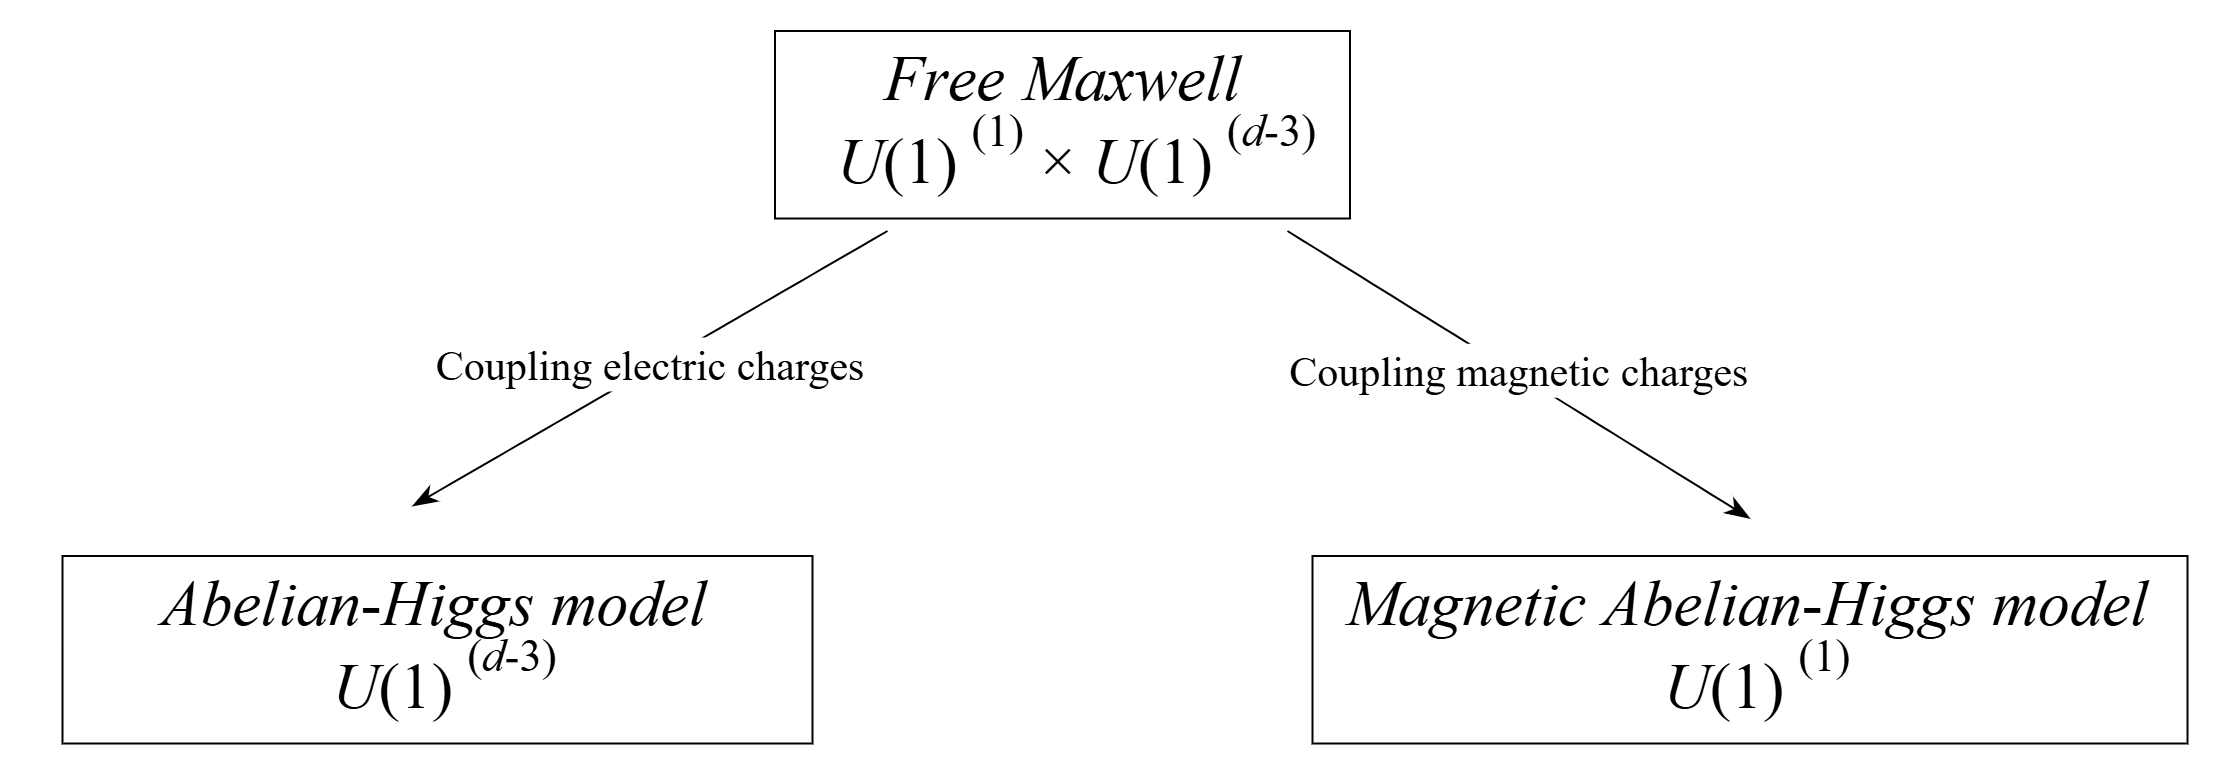
\includegraphics[width=0.75\linewidth]{images/maxwell_coupling.png}
    \caption{Map of theories we obtain coupling dynamical electric/magnetic charges to free Maxwell theory, together with the residual symmetries they have.}
    \label{fig:coupling_maxwell}
\end{figure}

\subsubsection{The Special Case of Four Dimensions}
\label{subsec:four_dimensions}

A unique algebraic simplification occurs when setting $d=4$. In four dimensions, the degree of the magnetic symmetry group collapses from $U(1)^{(d-3)}_m$ to $U(1)^{(1)}_m$. Consequently, both the electric and magnetic generalized global symmetries are $1$-form symmetries:
\begin{equation}
U(1)_e^{(1)} \qquad \& \qquad U(1)^{(1)}_m
\end{equation}
Both the Wilson lines $W(\mathcal{M}_1)$ and the 't Hooft lines $T(\mathcal{M}_{1})$ operate as $1$-dimensional charged line operators. 
Furthermore, in this scenario the photon and the dual photon are both $1$-form gauge fields; in fact, the duality in this case is a self-duality.

\subsubsection{The Special Case of Three Dimensions}
\label{subsec:three_dimensions}
In $d=3$ dimensions, the magnetic symmetry group degree shifts to $d-3 = 0$, which is anticipated to manifest as a $0$-form global symmetry $U(1)_m^{(0)}$. While coupling the theory to an electrically charged scalar field $\phi$ explicitly breaks the $1$-form electric symmetry $U(1)_e^{(1)}$, addressing the system in the presence of magnetic defects is understood to necessitate the dual photon formulation. Here, the dual field strength is a $1$-form $g^{(1)} = \star f^{(2)} = d\tilde{a}^{(0)}$, where the dual photon $\tilde{a}^{(0)}$ acts as a compact $0$-form scalar field.

The introduction of magnetic charges—treated as point-like spacetime instantons—is expected to deform the theory via non-local monopole operators $V_{\pm}(x) \sim e^{\pm i \tilde{a}^{(0)}(x)}$. This non-perturbative instanton potential $V(\tilde{a}^{(0)})$ should explicitly break the continuous $U(1)_m^{(0)}$ shift symmetry down to a discrete subgroup. Prior to any condensation mechanism, the $1$-form electric symmetry $U(1)_e^{(1)}$ should remain protected by the topological constraint $d \star f^{(2)} = d d\tilde{a}^{(0)} = 0$. The vacuum dynamics of these configurations are conjectured to isolate two macroscopically distinct regimes.
\paragraph*{The Symmetric Phase: The Coulomb Phase}When topological magnetic defects remain dilute and un-condensed, the infrared (IR) effective action should be governed purely by the free gauge kinetic term:
\begin{equation}
\mathcal{S}_{\text{EFT}}[a^{(1)}] = \frac{1}{2e_{\text{eff}}^2} \int_{\mathcal{M}_3} f^{(2)} \wedge \star f^{(2)}.
\end{equation}
In this Coulomb phase, the $1$-form electric symmetry $U(1)_e^{(1)}$ is conjectured to undergo spontaneous symmetry breaking, yielding an emergent $U(1)_m^{(0)}$ symmetry in the deep IR. Consequently, the non-local Wilson line operators are expected to obey a perimeter law, as we mentioned in \ref{sec:landau_paradigm},
\begin{equation}
\langle W(\mathcal{M}_1) \rangle \sim \exp\left(-\alpha \cdot \text{Perimeter}(\mathcal{M}_1)\right),
\end{equation}
consistent with the deconfinement of electric excitations. Concurrently, local 't Hooft operators should exhibit long-range order dictated by the massless dual scalar propagator:
\begin{equation}
\langle T(x) T^\dagger(y) \rangle \sim \exp\left( \frac{e_{\text{eff}}^2}{4\pi |x-y|} \right) \xrightarrow{|x-y| \to \infty} \text{constant} \neq 0.
\end{equation}
By cluster decomposition,\footnote{We evaluate the un-subtracted correlation function where $\langle \mathcal{O}(x) \mathcal{O}(y) \rangle \sim \langle \mathcal{O}(x) \rangle \langle \mathcal{O}(y) \rangle$ at asymptotic separation, bypassing the trivially vanishing connected components.} this behavior would signal the spontaneous breaking of the emergent magnetic symmetry, with the massless $1$-form photon $a^{(1)}$ acting as the associated Nambu-Goldstone boson.

\paragraph*{The Condensed Phase: The Dual Superconducting Phase or Superinsulator}
Conversely, upon the condensation of magnetic monopoles, the system is expected to undergo a quantum phase transition where the dual photon $\tilde{a}^{(0)}$ develops a mass gap via the instanton-induced potential, gapping the long-range gauge degrees of freedom.

In this scenario, the magnetic condensate should shield the vacuum against the screening of electric fields, thereby restoring the exact $1$-form electric symmetry $U(1)_e^{(1)}$ to an unbroken state. As a direct diagnostic of this unbroken higher-form symmetry, the Wilson loop expectation value is anticipated to transition to an area law:\begin{equation}\langle W(\mathcal{M}_1) \rangle \sim \exp\left(-\sigma \cdot \text{Area}(\mathcal{M}_2)\right), \quad \partial\mathcal{M}_2 = \mathcal{M}_1.\end{equation}This configuration would realize the Polyakov-Mandelstam-`t Hooft confinement mechanism in $3d$, where monopole condensation dualizes the conventional Meissner effect, collimating electric field lines into isolated flux tubes and enforcing the confinement of electric test charges.

\subsubsection{The SymTFT POV}
Given the $XY$-model \ref{eq:xy_model}, with a $U(1)^{(0)}$ symmetry, its SymTFT is
\begin{equation}\label{eq:symtft_xy_model}
    \mathcal{S}^{XY}_{SymTFT} = \frac{i}{2\pi} \int_{\mathcal{Y}_4} b^{(2)} \wedge dA^{(1)}
\end{equation}
which in its SSB phase gives the Superfluid Theory  \ref{eq:superfluid}, with a $U(1)^{(0)} \times U(1)^{(1)}$ symmetry and a mixed anomaly. Its SymTFT is
\begin{equation}
    \mathcal{S}^{SF}_{SymTFT} = \frac{i}{2\pi} \int_{\mathcal{Y}_4} b^{(2)} \wedge dA^{(1)} + c^{(1)} \wedge dB^{(2)} - B^{(2)} \wedge dA^{(1)}
\end{equation}
gauging its $U(1)^{(0)}$ symmetry we expect to obtain Superconductor theory (Higgs phase) which is dual to the unbroken phase of the XY-model, we expect then to obtain \ref{eq:symtft_xy_model}.

Let us apply the tools we developed in \ref{sec:symtft_continuous_gauging}, taking the substitution
\begin{equation}
    dA^{(1)} \to f^{(2)} \qquad \& \qquad b^{(2)} \to dC^{(1)}
\end{equation}
obtaining the dynamical gauged SymTFT
\begin{equation}
    \mathcal{S}^{SF}_{SymTFT} = \frac{i}{2\pi} \int_{\mathcal{Y}_4} dC^{(1)} \wedge f^{(2)} + c^{(1)} \wedge dB^{(2)} - B^{(2)} \wedge f^{(2)}
\end{equation}
Varying the gauged action $\mathcal{S}^{\text{SF}}_{\text{SymTFT}}$ with respect to the fields yields the complete set of bulk equations of motion: 
\begin{align}
    \delta C^{(1)}: & \quad df^{(2)} = 0  \qquad & \qquad
    \delta c^{(1)}: & \quad dB^{(2)} = 0  \\
    \delta f^{(2)}: & \quad dC^{(1)} - B^{(2)} = 0   \qquad & \qquad
    \delta B^{(2)}: & \quad dc^{(1)} + f^{(2)} = 0 
\end{align}

The appearence of the non-derivative term implies that we have to redefine the gauge transformations. Let us take the gauge transformations 
\begin{equation}
    \delta C^{(1)} = d\Lambda_C + K_C \qquad 
    \delta f^{(2)} = d\Lambda_f + K_f \qquad 
    \delta c^{(1)} = d\Lambda_c + K_c \qquad 
    \delta B^{(2)} = d\Lambda_B + K_B
\end{equation}
then
\begin{multline}
    \delta \mathcal{L}^{SF}_{SymTFT} \sim 
    d \delta C^{(1)} \wedge f^{(2)} +  \delta c^{(1)} \wedge dB^{(2)} -  \delta B^{(2)} \wedge f^{(2)} 
    + dC^{(1)} \wedge  \delta f^{(2)} + c^{(1)} \wedge d \delta B^{(2)} - B^{(2)} \wedge  \delta f^{(2)} + \\ 
    + d \delta C^{(1)} \wedge  \delta f^{(2)} +  \delta c^{(1)} \wedge d \delta B^{(2)} -  \delta B^{(2)} \wedge  \delta f^{(2)} \\
    = d K_C \wedge f^{(2)} +  (d\Lambda_c + K_c) \wedge dB^{(2)} -  (d\Lambda_B + K_B) \wedge f^{(2)} +\\
    + dC^{(1)} \wedge  (d\Lambda_f + K_f) + c^{(1)} \wedge d K_B - B^{(2)} \wedge  (d\Lambda_f + K_f) + \\ 
    + d K_C \wedge  (d\Lambda_f + K_f) +  (d\Lambda_c + K_c) \wedge d K_B -  (d\Lambda_B + K_B) \wedge  (d\Lambda_f + K_f) \\
    = d K_C \wedge f^{(2)} +  K_c \wedge dB^{(2)} -  d\Lambda_B  \wedge f^{(2)} -  K_B \wedge f^{(2)} +\\
    + dC^{(1)} \wedge  K_f + c^{(1)} \wedge d K_B - B^{(2)} \wedge  d\Lambda_f - B^{(2)} \wedge   K_f + \\ 
    + d K_C \wedge  K_f +  K_c \wedge d K_B -  d\Lambda_B  \wedge   K_f -   K_B \wedge  d\Lambda_f  - K_B\wedge K_f 
\end{multline}
The terms we cannot allow are $-  d\Lambda_B  \wedge f^{(2)}$ and $- B^{(2)} \wedge  d\Lambda_f$, the first one imposes $K_C =  \Lambda_B$ and the second imposes $K_c = - \Lambda_f$. On the other hand, $K_B=K_f=0$.

We thus obtain the gauge transformations
\begin{align}\label{eq:gauge_transf_abj}
   \delta C^{(1)} = d\Lambda_C + \Lambda_B \qquad 
    \delta f^{(2)} = d\Lambda_f  \qquad 
    \delta c^{(1)} = d\Lambda_c + \Lambda_f \qquad 
    \delta B^{(2)} = d\Lambda_B  
\end{align}

Keeping this into account, we look at the operator content of the theory. First we have
\begin{equation}
    V^f_\alpha (\Gamma) = e^{i\alpha \int_\Gamma f} \qquad \& \qquad W^B_n (\Gamma) = e^{in\int_\Gamma B}
\end{equation}
where $\Gamma$ is a $2d$ submanifold, $\alpha \in \mathbb{R}$ and $n \in \mathbb{Z}$. Their topological property is ensured by the EOM: $df=dB=0$ (flat curvatures, as we expect from TQFT).
On the other hand, we cannot do the same for $C, c$ because of \ref{eq:gauge_transf_abj}, however we can build non-gennuine topological operators:
\begin{equation}
    \tilde{U}^c_\alpha (\gamma, D) = e^{i\alpha( \int_\gamma c -\int_D f)} \qquad \& \qquad \tilde{T}^C_n (\gamma, D) = e^{in(\int_\gamma C + \int_D B)}
\end{equation}
where $\gamma$ is $1d$ and $D$ is $2d$.


\begin{tcolorbox}[colback=blue!5!white,colframe=blue!75!black,title={Proposal}]
    We now want to propose a $1d$ edge modes theory to use when dressing the defect in order to make it genuine. 

    The dressed defect $\tilde{U}^c_\alpha (\gamma, D)$ would take the form
    \begin{equation}
        \mathcal{D}_\frac{2\pi}{N} = \int \mathcal{D} a^{(1)} \mathcal{D} \lambda^{(0)}\exp \left[ i  \int_{\gamma} \frac{2\pi}{N} c^{(1)} +  2\pi a^{(1)} + \frac{\lambda^{(0)}}{2\pi}\left(b^{(1)} +  Na^{(1)} \right) \right]
    \end{equation}
    where $f^{(2)} = db^{(1)}$ locally.

    This proposal is problematic because the second term does not posses the right quantization condition, it is indeed non gauge invariant. This logic crosses out the proposal.
\end{tcolorbox}

We conclude by saying that the gauging process has made non genuine two of the topological operators in the SymTFT, thus making them trivially contractible.


%%%%%%%%%%%%%%%%%%%%%%%%%%%%%%%%%%%%%%%%%%%%%%%%%%%%%%%%%%%%%%%%%%%%%%%%
%%%%%%%%%%  Goldstone Model - Superfluid + Topological term  %%%%%%%%%%%
%%%%%%%%%%%%%%%%%%%%%%%%%%%%%%%%%%%%%%%%%%%%%%%%%%%%%%%%%%%%%%%%%%%%%%%%

\subsection{Superfluid + Topological term model}
\label{sec:superfluid_topologicalterm}
{\bf In this section we analyze a particular theory with the intent of understanding better the $3d$ complex scalar boson and its emergent symemtry in the SSB phase. In fact, we are studying its SSB phase with a particular topological coupling. Although the following theory is not directly related to the one of our interest, it is preparatory for the next one.}

In this sections, we analyze the model of a Nambu-Goldstone mode WRT a SSB $U(1)^{(0)}_A$ phase symmetry, namely the theory of superfluids in $3d$, on $\mathcal{M}_3$.

The Goldstone DOF transforms non-linearly under a symmetry operation: $\chi \to \chi + \alpha$. With the DOF that we have at our disposal, including the background field for the $U(1)^{(0)}_A$ symmetry, we can also have a topological term: 

\begin{equation}
\mathcal{S}[\chi^{(0)} ; B_A^{(1)}, B_B^{(2)}, \theta] = \frac{1}{2}\int (d\chi - B_A)\wedge \star (d\chi - B_A) + \frac{i\theta}{4 \pi^2} \int d\chi \wedge F_A + \frac{i}{2 \pi} \int d\chi \wedge B_B 
\end{equation}

Where the first term is the kinetical term for the Goldstone mode coupled non linearly with the $U(1)^{(0)}_A$ background field $B_A$, the second is the topological term we are allowed to include\footnote{We could perform a similar procedure WRT the other symmetry, inserting $ \theta ' \int \star d\chi \wedge F_B$.} and the third is the standard coupling to a background field for the $U(1)^{(1)}_B$ symmetry.

As well known, the Superfluid theory has an extra emergent $U(1)^{(1)}_B$ symmetry\footnote{WRT the unbroken $U(1)^{(0)}_A$ parent theory.} whose symmetry charge operator counts the winding excitations. Thus, the symmetry currents are\footnote{Including an explicit factor of $-i$ in $j^{(1)}_A$ ensures that the anomalous contribution in the conservation equation remains purely real in Euclidean signature.}
\begin{equation}
j^{(1)}_A = -i d \chi \qquad \& \qquad j^{(2)}_B = \frac{1}{2 \pi} \star d \chi
\end{equation}

Furthermore, the Superfluid theory possesses a mixed anomaly between the two symmetries
\begin{equation}
\mathcal{Z}[\chi ; B_A + d\Lambda_A, B_B + d\Lambda_B, \theta] = \exp \left(  \frac{i}{2\pi} \int_{\mathcal{M}_3} \Lambda_A \wedge F_B  \right) \times\mathcal{Z}[\chi ; B_A, B_B, \theta]
\end{equation}

We can collect the information of the anomaly within the anomaly polynomial
\begin{equation}
\mathcal{I}_5 = -\frac{i}{2\pi} F_A \wedge F_B
\end{equation}

Moreover, given the normalizations $\oint_{\mathcal{M}_1}d\chi=2\pi \mathbb{Z}$ and $\oint_{\mathcal{M}_2} F_A =2\pi \mathbb{Z}$ for any $\mathcal{M}_1$ and $\mathcal{M}_2$, we notice that the parameter $\theta$ is periodic, i.e. has a $\mathbb{Z}$ shift symmetry $\theta \to \theta + 2\pi$. 

{\bf We now promote $\theta$ as a spacetime dependent background field WRT the $-1$-form symmetry given by $\star j^{(0)}_C = d\chi \wedge F_A$.\footnote{This Noether current operator contains a background non-dynamical field, it does not represent a symmetry, it is not an operator.}} 

Notice that, promoting $\theta$ to a field produces the effect of modifying the EOM:
\begin{equation}
-d\star(d\chi - B_A) + \frac{i}{4\pi^2}d\theta\wedge F_A + \frac{i}{2\pi}F_B = 0
\end{equation}
Substituting $\star j_A = -i \star(d\chi - B_A)$ transforms this equation directly into the anomalous conservation law for the $U(1)^{(0)}_A$ symmetry:
\begin{equation}
d\star j_A = \frac{1}{4\pi^2}d\theta \wedge F_A + \frac{1}{2\pi}F_B
\end{equation}
which means that the symmetry $U(1)^{(0)}_A$ is involved in an anomaly.

For the winding symmetry, the dualized current is $\star j_B = \frac{1}{2\pi}d\chi$, which yields $d\star j_B = 0$ identically. Both currents satisfy the $d\star j = 0$ closure condition when background fields vanish and $\theta$ is constant.


We can include this anomaly in the anomaly polynomial, obtaining 
\begin{equation}
\mathcal{I}_5 = -\frac{i}{2\pi} F_A \wedge F_B - \frac{1}{4 \pi^2} d\theta \wedge F_A \wedge F_A
\end{equation}
Notice the similarity of the second term with the anomaly polynomial of the theory of massless fermion before we coupled to QED, in \ref{sec:abj_example}, manifesting a mixed 't Hooft anomaly that after gauging results into the famous ABJ-symmetry breaking. Look at \ref{sec:engineer_non-inv}. The difference is that we will gauge the $-1$-form symmetry instead of the $0$-form symmetry.

\subsubsection{Gauging of the $-1$-form symmetry}
\label{sec:superfluid_00_composite}
{\bf A new theory: promote $\theta$ to a dynamical $U(1)$-valued field $\phi$.} 

This means we introduce a new kinetic term for the new field $\int d\phi \wedge \star d\phi$. This procedure erase the $-1$-form symmetry we gauged and affects all the symmetries that were involved in a mixed anomaly with it. Furthermore, this modification of the theory introduces two new symmetries:\footnote{As every higher-form Superfluid does \cite{Delacr_taz_2020}.} $U(1)^{(0)}_C$ and $U(1)^{(1)}_D$, whose currents are
\begin{equation}
j^{(1)}_C = -id\phi \qquad \& \qquad j^{(2)}_D = \frac{1}{2\pi}\star d\phi
\end{equation}

The new theory has action, keeping active only the background for $U(1)^{(0)}_A$ 
\begin{align}
\mathcal{S}[\chi^{(0)}, \phi^{(0)}; B_A^{(1)}] = & \frac{1}{2}\int (d\chi - B_A) \wedge \star (d\chi - B_A)  +\frac{1}{2}\int d\phi \wedge \star d\phi  + \frac{i}{4 \pi^2} \int \phi \wedge d\chi \wedge F_A  
\end{align}


\begin{tcolorbox}
    {\bf A different point of view}
    
    The just presented theory has also a different interpretation. Imagine to have two species of superfluids, $\chi$ and $\phi$. Both of them have two symmetries, in particular we have $\star j^{(2)}_D = \frac{1}{2\pi}  d\phi$ and $\star j^{(2)}_B = \frac{1}{2\pi}  d\chi$. Given them we can build a new composite (or Chern-Weil \cite{Heidenreich_2021}) closed form $\star j^{(1)}_E = \star j^{(2)}_D \wedge \star j^{(2)}_B$. Moreover, we can turn on a background gauge field for this composite symmetry which we will call $B^{(1)}_E$.
    
    The term of interest looks like
    \begin{equation}
        -\frac{i}{4\pi} \int d\phi \wedge d\chi \wedge B_E
    \end{equation}
    To connect to what the authors of \cite{Damia_2023} did, and I reported above, we need to take a further step and set equal $B_A = B_E$ (and integrate by parts). Since what follows is independent of this choice, I will take the perspective described here.
\end{tcolorbox}

If we then activate all the others background fields for the various symmetries we obtain
\begin{align}
\mathcal{S}[\chi, \phi ; B_A,.., B_E ] = & \frac{1}{2}\int (d\chi - B_A)\wedge \star (d\chi - B_A) +\frac{1}{2}\int (d\phi - B_C)\wedge \star (d\phi - B_C) \\
&- \frac{i}{4 \pi^2} \int d\phi \wedge d\chi \wedge B_E + \frac{i}{2 \pi} \int d\chi \wedge B_B + \frac{i}{2 \pi} \int d\phi \wedge B_D 
\end{align}

By evaluating the functional variation of the Euclidean action $\mathcal{S}$ with respect to the Goldstone mode $\chi$ and the Axion $\phi$, the equation of motions yield:
\begin{align}
    -d\star(d\chi - B_A) + \frac{i}{4\pi^2}d\phi\wedge F_E + \frac{i}{2\pi}F_B = 0 \\
    -d\star(d\phi - B_C) - \frac{i}{4\pi^2}d\chi \wedge F_E + \frac{i}{2\pi}F_D = 0
\end{align}

Substituting $\star j_A = -i \star(d\chi - B_A)$ and $\star j_C = -i \star(d\phi - B_C)$ this equations transform directly into the anomalous conservation laws for the $U(1)^{(0)}_A$ and $U(1)^{(0)}_C$ symmetries:
\begin{align}\label{eq:superfluid_topo_cons_eq}
    d\star j_A &= \frac{1}{4\pi^2}d\phi \wedge F_E + \frac{1}{2\pi}F_B \qquad 
    & d\star j_C &= -\frac{1}{4\pi^2}d\chi \wedge F_E + \frac{1}{2\pi}F_D
    \\
    &= \frac{1}{2\pi} \star j_D\wedge F_E + \frac{1}{2\pi}F_B \qquad 
    & &= -\frac{1}{2\pi} \star j_B\wedge F_E + \frac{1}{2\pi}F_D 
\end{align}
For the winding symmetries, the dualized currents yields $d\star j_B = d\star j_D  = 0$ identically. All the four currents satisfy the $d\star j = 0$ closure condition when background fields vanish.

Looking at the conservation equations \ref{eq:superfluid_topo_cons_eq}, we notice that that the anomalous conservation involves dynamical fields in the exact way that manifests an higher group structure, i.e. there is a operator valued shift as we discussed in \ref{sec:mixed_anomaly_to_gen_sym}. In fact, (taking the old perspective) since the $U(1)^{(0)}_A$ symmetry was involved in the anomaly, after gauging the $-1$-form symmetry it gets modified. we obtain a $2$-group structure. 
We can see it by the standard procedure, look at the terms of the lagrangian
\begin{equation}
    \mathcal{L} \supset \star j_B \wedge B_B + \star j_C \wedge B_C 
\end{equation}
performing a variation of all the background fields and permitting a correction to the shift of the form $\delta B_i = d\Lambda_i + K_i$
\begin{align}
    \star j_B \wedge \delta B_B + \star j_C \wedge \delta B_C  
    &= \star j_B \wedge (d\Lambda_B + K_B) + \star j_C \wedge (d\Lambda_C + K_C)  \\
    &= -d\star j_B \wedge \Lambda_B + \star j_B \wedge K_B - d \star j_C \wedge \Lambda_C + \star j_C \wedge K_C  \\
    &= \star j_B \wedge K_B - d \star j_C \wedge \Lambda_C + \star j_C \wedge K_C  \\
    &= \star j_B \wedge K_B - \left(\frac{1}{2\pi} \star j_B\wedge F_E + \frac{1}{2\pi}F_D\right) \wedge \Lambda_C + \star j_C \wedge K_C  \\
    &= \star j_B \wedge \left( K_B - \frac{1}{2\pi} F_E \wedge \Lambda_C\right) 
\end{align}
where in the first line we just substituted, in the second integrated by parts, in the third used the conservation equation for $j_B$, in the fourth substituted the non conservation equation for $j_C$, and in the last we kept only the operator valued shift to be corrected and  setting $K_C = 0$. We thus obtain $K_B = \frac{1}{2\pi} F_E \wedge \Lambda_C$ for the theory to be well defined. Analogously we can analyze the term
\begin{equation}
    \mathcal{L} \supset \star j_A \wedge B_A + \star j_D \wedge B_D 
\end{equation}
and following the same steps we obtain
\begin{equation}
    \star j_A \wedge \delta B_A + \star j_D \wedge \delta B_D = \star j_D \wedge \left( K_D + \frac{1}{2\pi} F_E \wedge \Lambda_A\right)
\end{equation}
which forced us to impose $K_D = -\frac{1}{2\pi} F_E \wedge \Lambda_A$. 

Explicitly, we need to modify the background gauge transformations for $U(1)^{(1)}_B$ and $U(1)^{(1)}_D$:
\begin{equation}
B_B \to B_B + d\Lambda_B + \frac{1}{2\pi}\Lambda_C \wedge F_E \qquad \& \qquad B_D \to B_D + d\Lambda_D - \frac{1}{2\pi}\Lambda_A \wedge F_E
\end{equation}

The same information, i.e. the symmetry structure being a $2$-group, can be encoded in the modified Bianchi identities\footnote{Here we have redefined the curvatures $F$ such that they are gauge invariant WRT the new gauge transformations; but this leads to loosing the closure property \cite{C_rdova_2019}.}
\begin{equation}
dF^{(3)}_B = \frac{1}{2\pi} F^{(2)}_C \wedge F^{(2)}_E \qquad \& \qquad dF^{(3)}_D = -\frac{1}{2\pi} F^{(2)}_A \wedge F^{(2)}_E
\end{equation}

The anomaly polynomial is
\begin{equation}\label{eq:anomaly_poly_2superfluids}
\mathcal{I}_5 = -\frac{i}{2\pi} F^{(2)}_A \wedge F^{(3)}_B - \frac{i}{2\pi} F^{(2)}_C \wedge F^{(3)}_D
\end{equation}
and we can check it is still closed
\begin{align}
    d \mathcal{I}_5 
    =&-\frac{i}{2\pi} F_A \wedge dF_B - \frac{i}{2\pi} F_C \wedge dF_D \\
    =&-\frac{i}{4\pi^2} F_A \wedge F_C \wedge F_A + \frac{i}{4\pi^2} F_C \wedge F_A \wedge F_A =0\\
\end{align}

{\bf This model teaches us that if we turn on the background gauge field for the composite $0$-form symmetry $\star j^{(1)}_E = \star j^{(2)}_D \wedge \star j^{(2)}_B$ where $j_D, j_B$ are the winding symmetries of our two copies of superfluid, then we notice a $2$-group structure in the model.}

This theory connects to the following in multiple ways, one of them is this: dynamically gauging the composite symemtry, i.e. making $B_E$ dynamical, gives us the theory \ref{sec:superfluid_01_composite}.

%%%%%%%%%%%%%%%%%%%%%%%%%%%%%%%%%%%%%%%%%%%%%%%%%%%%%%%%%%%%%%%%%%%%%%%%
%%%%%%%%%%%%%%%%%%  Goldstone-Maxwell Model  %%%%%%%%%%%%%%%%%%%%%%%%%%%
%%%%%%%%%%%%%%%%%%%%%%%%%%%%%%%%%%%%%%%%%%%%%%%%%%%%%%%%%%%%%%%%%%%%%%%%

\subsection{Goldstone-Maxwell Model}
{\bf With the idea of looking for non-invertible generalized symmetries in the $3d$ complex scalar boson such that they relate to the emergent symemtry in the Superfluid phase, we analyze this theory. Again, this model does not relate directly to the theory of our interest, but a gauged version of it will, as we will see.}

The following theory relates to the one of our interest in the following way: take two copies of $3d$ Superfluids, use particle-vortex duality on one of them obtaining free Maxwell theory,\footnote{The first term might not seem a Superfluid, but it is. Recall we discussed the duality between free Maxwell theory and Superfluid in $3d$ in \ref{sec:complex_boson_3d}.} and turn on a topological coupling between them using the $0$-form symmetry of one of them and the $1$-form symmetry of the other.\footnote{Notice the difference with the model discussed in \ref{sec:superfluid_00_composite}, where we build a composite closed current out of the two $0$-form symmetries.}

We now consider the following theory
\begin{equation}
\mathcal{S}[\chi, f;\theta] = \frac{1}{2 g^2} \int f \wedge \star f + \frac{1}{2} \int d\chi \wedge \star d\chi + \frac{i \theta}{4 \pi^2} \int d\chi \wedge f
\end{equation}
with the following EOM (here we are already considering the spacetime dependence of $\theta$)
\begin{align}
    -\frac{1}{g^2}d\star f - \frac{i}{4\pi^2} d\theta \wedge d\chi = 0 \\
    -d\star d \chi - \frac{i}{4\pi^2} d\theta \wedge f = 0
\end{align}

The theory has the following symmetry currents\footnote{We are not considering the improvements given by the $\theta$ term.}
\begin{align}
    j^{(1)}_A = -id\chi \qquad j^{(2)}_B = \frac{1}{2\pi}\star d\chi \qquad j^{(1)}_C = \frac{1}{2\pi} \star f \qquad j^{(2)}_D = -\frac{i}{g^2} f
\end{align}

If we now decide to repeat the philosopy of the previous example, i.e. making $\theta$ spacetime dependent as a background field for a $-1$-form symmetry, we can probe the anomalies in which this symemtry is involved.

\begin{tcolorbox}
    {\bf The composite current}
    
    Again, we should take a closed look at the topological coupling. In fact, promoting $\theta$ to be spacetime dependent, it can be rewritten as
    \begin{equation}
        +i\int \theta \wedge \star j_B \wedge \star j_C
    \end{equation}
    which allows us to reinterpret it as the background gauge field $\theta$ coupled to the composite $-1$-form symmetry current $\star j^{(0)}_E = \star j^{(2)}_B \wedge \star j^{(1)}_C$.
\end{tcolorbox}

In fact,
\begin{align}
d\star j^{(1)}_A &= - \frac{1}{4\pi^2} d\theta \wedge f & d \star j^{(2)}_D &= - \frac{1}{4 \pi^2} d\theta \wedge d\chi \\
&= - \frac{1}{2\pi} d\theta \wedge \star j_C & &= - \frac{1}{2\pi} d\theta \wedge \star j_B
\end{align}
This shows the non-conservation of the two currents in the presence of a non flat background for the composite $-1$-form symmetry.

Notice that the non-conservation equations have the exact form of the ones that give a higher-group structure, as discussed in \ref{sec:mixed_anomaly_to_gen_sym} and also pointed out in \cite{Brauner_2021}. In fact, looking at the part of the lagrangian with background coupling
\begin{equation}
    \mathcal{L} \supset \star j_A \wedge B_A + \star j_C \wedge B_C
\end{equation}
by the standard procedure we obtain
\begin{equation}
    \star j_A \wedge \delta B_A + \star j_C \wedge \delta B_C = \star j_C \wedge ( \frac{1}{2\pi} d\theta \wedge \Lambda_A + K_C ) 
\end{equation}
and analogously for $j_B, j_D$
\begin{equation}
    \star j_D \wedge \delta B_D + \star j_B \wedge \delta B_B = \star j_B \wedge ( -\frac{1}{2\pi} d\theta \wedge \Lambda_D + K_B ) 
\end{equation}
obtaining the higher group structure encoded in
\begin{equation}
    dF_B = \frac{1}{2\pi} d\theta \wedge F_D \qquad \& \qquad dF_C = -\frac{1}{2\pi} d\theta \wedge F_A
\end{equation}
The theory has the same anomaly polynomial that we wrote in \ref{eq:anomaly_poly_2superfluids} since we are looking at the same theory, just with a different background turned on WRT a different composite symmetry.

\subsubsection{Gauging of the $-1$-form symmetry}
\label{sec:superfluid_01_composite}

Let us now gauge the $-1$-form symmetry, i.e. we promote $\theta$ to a dynamical DOF $\phi$ and adding its kinetic term. We obtain the theory
\begin{equation}
\mathcal{S}[\chi^{(0)}, f^{(2)}, \phi^{(0)}] = \frac{1}{2 g^2} \int f \wedge \star f + \frac{1}{2} \int d\chi \wedge \star d\chi + \frac{1}{2} \int d\phi \wedge \star d\phi + \frac{i }{4 \pi^2} \int \phi \wedge d\chi \wedge f
\end{equation}
The last term can be manipulated, we can rewrite it as $- \frac{i }{4 \pi^2} \int d\phi \wedge d\chi \wedge a^{(1)}$, where $da=f$, or $- \frac{i }{4 \pi^2} \int d\phi \wedge \chi \wedge f$; this should clarify that $\chi$ and $\phi$ are on the same footing. Furthermore, it should clarify that we can interpret this theory in two different ways:
\begin{enumerate}[\itshape i)]
    \item Two copies of Superfluid in their scalar description with the composite $0$-form symemtry given by their $1$-form symemtries, gauged; taking the theory \ref{sec:superfluid_00_composite} and making $B_E$ dynamical.
    \item Two copies of Superfluid, one in the scalar description and one in the Maxwell description, with the composite $-1$-form symmetry given by a $1$-form symmetry and a $0$-form symemtry, gauged.
\end{enumerate}

Its EOM are, taking the variation in the order $\chi, f, \phi$ respectively,
\begin{align}
    -d\star d \chi - \frac{i}{4 \pi^2} d\phi \wedge f = 0 \\
    - \frac{1}{g^2} d\star f - \frac{i}{4 \pi^2} d\phi \wedge d\chi = 0 \\
    -d\star d \phi +  \frac{i}{4 \pi^2} d\chi \wedge f = 0
\end{align}
Defining the following forms (with the idea of recalling the corresponding would be symmetries) 
\begin{align}
    j^{(1)}_A &= -id\chi  & j^{(2)}_B &= \frac{1}{2\pi}\star d\chi \\
     j^{(1)}_C &= \frac{1}{2\pi} \star f  & j^{(2)}_D &= -\frac{i}{g^2} f \\
     j^{(1)}_E &= -id\phi  & j^{(2)}_F &= \frac{1}{2\pi}\star d\phi
\end{align}
we can see immediately that $d\star j_B = d\star j_C = d\star j_F = 0$ (in absence of monopoles) from the formalism, i.e. $dd\omega = 0 \quad \forall\omega$, and from the EOM we see that three of them fail to be closed
\begin{align}
    d \star j^{(1)}_A &= -\frac{1}{4 \pi^2} d\phi \wedge f \\
    d \star j^{(2)}_D &= -\frac{1}{4 \pi^2} d\phi \wedge d \chi \\
    d\star j^{(2)}_E &= +\frac{1}{4 \pi^2} d\chi \wedge f
\end{align}

We want now to build the symemtry operators WRT these non-conserved currents. The would be symmetry operator $U=e^{i\alpha \int \star j}$ is no more topological since $\star j$ is not closed. We can thus define
\begin{align}
    U^A_\alpha (\mathcal{M}_2) &= \exp \left(  i \alpha \int \star j_A + \frac{1}{4 \pi^2} \phi \wedge f\right) \\
    U^D_\beta (\mathcal{M}_1) &= \exp \left(  i \beta \int \star j_D + \frac{1}{4 \pi^2} \phi \wedge d\chi \right) \\
    U^E_\gamma (\mathcal{M}_2) &= \exp \left(  i \gamma \int \star j_E - \frac{1}{4 \pi^2} \chi \wedge f \right)
\end{align}
these operators are topological, but not gauge invariant for all the values of $\alpha , \beta, \gamma$, and restricting to the allowed values would lead to trivial operators or symmetry operators without any charged object.

It happens that for $\alpha , \beta, \gamma = 2\pi / N$ we can do better \cite{Damia_2023}, following the original idea of \cite{choi2022noninvertibleglobalsymmetriesstandard, cordova2022noninvertiblechiralsymmetryexponential}. We can construct a BF-theory living on the symmetry defect allowing for fractional phase rotations
\begin{align}
    \mathcal{D}^A_{\frac{1}{N}} (\mathcal{M}_2) = \int \mathcal{D}\xi^{(0)} \mathcal{D}v^{(1)} \exp \left(  i  \int_{\mathcal{M}_2} \frac{2 \pi}{N} \star  j_A + \frac{N}{2 \pi} \xi \wedge dv + \frac{1}{2 \pi} \xi \wedge f - \frac{1}{2 \pi} \phi \wedge dv \right) \\
    \mathcal{D}^D_{\frac{1}{M}} (\mathcal{M}_1) = \int \mathcal{D}\xi^{(0)} \mathcal{D}\rho^{(0)} \exp \left(  i  \int_{\mathcal{M}_1} \frac{2 \pi}{M} \star  j_D + \frac{M}{2 \pi} \xi \wedge d\rho + \frac{1}{2 \pi} \xi \wedge d\chi - \frac{1}{2 \pi} \phi \wedge d\rho \right) \\
    \mathcal{D}^E_{\frac{1}{K}} (\mathcal{M}_2) = \int \mathcal{D}\xi^{(0)} \mathcal{D}v^{(1)} \exp \left(  i  \int_{\mathcal{M}_2} \frac{2 \pi}{K} \star  j_E + \frac{K}{2 \pi} \xi \wedge dv + \frac{1}{2 \pi} \xi \wedge f - \frac{1}{2 \pi} \chi \wedge dv \right)
\end{align}
where $\xi, \rho$ are compact scalars and $v$ is a $1$-form gauge field, all of them living only on the defect. In the first and third case we dressed $U^A_{\frac{2\pi}{N}} (\mathcal{M}_2)$ and $U^E_{\frac{2\pi}{K}} (\mathcal{M}_2)$ with a $2d$ BF-theory, and in the second case we dressed $U^D_{\frac{2\pi}{M}} (\mathcal{M}_1)$ with a $1d$ BF-theory.\footnote{These two theories can be understood as sequential reduction, i.e. projecting on a lower dimensional manifold, of the $3d$ Fractional Quantum Hall theory \cite{Damia_2023}.} 

The two defects are non invertible, in fact they are not even unitary; we can see it by building their conjugate counterparts $\mathcal{D}^A_{\frac{1}{N}} (\mathcal{M}_2)^\dagger$ and $\mathcal{D}^D_{\frac{1}{M}} (\mathcal{M}_1)^\dagger$, and fusing them. For example 
\begin{multline}
    \mathcal{D}^A_{\frac{1}{N}} (\mathcal{M}_2) \times \mathcal{D}^A_{\frac{1}{N}} (\mathcal{M}_2)^\dagger  = \\ 
     \int \mathcal{D}\Phi \exp \left(  i  \int_{\mathcal{M}_2}  \frac{N}{2 \pi} ( \xi \wedge dv - \bar \xi \wedge d \bar v)+ \frac{1}{2 \pi} (\xi - \bar \xi) \wedge f - \frac{1}{2 \pi} \phi \wedge (dv - d \bar v) \right)
\end{multline}
where $\mathcal{D}\Phi = \mathcal{D}\xi^{(0)} \mathcal{D}v^{(1)}  \mathcal{D}\bar\xi^{(0)} \mathcal{D}\bar v^{(1)}$; and similarly for $\mathcal{D}^D_{\frac{1}{M}} (\mathcal{M}_1) \times \mathcal{D}^D_{\frac{1}{M}} (\mathcal{M}_1)^\dagger$ and $\mathcal{D}^E_{\frac{1}{K}} (\mathcal{M}_2) \times \mathcal{D}^E_{\frac{1}{K}} (\mathcal{M}_2)^\dagger$. The product operator can be understood in the context of higher gauging as a condensation defect, i.e. we are gauging a subgroup $\mathbb{Z}_N$ of the original symmetry $U_A^{(0)}(1)$ (and respectively $U_D^{(1)}(1), U_E^{(1)}(0)$) but not in the entire space, only along the submanifold $\mathcal{M}_2$, where the defect is defined.

\begin{tcolorbox}[title={Conclusion}]
    The construction of discrete $\mathbb{Q}/\mathbb{Z}$ non-invertible defects via worldvolume $\text{BF}$ tracking is structurally insufficient for our target system. The problem does not reside in the reduction to rational angles, since similar techniques have been used to keep the irrational part, e.g. in \cite{Arbalestrier_2025}. 

Consequently, our analysis pivots to the dynamical gauging of a \textit{composite} symmetry within a $3d$ gauge-scalar theory to evaluate how a nominally broken global symmetry is retained when a degree of freedom is gapped out. Under standard mass deformations, the winding symmetry of a single scalar sector is explicitly broken, which conventionally trivializes its topological charge. Gauging the composite current modifies this outcome. 

Following Brauner \cite{Brauner_2021}, the composite current $j \sim  d\phi_1 \wedge d\phi_2$ of a multi-component system geometrically measures the non-collinearity of the respective superflows. In $d=3$ dimensions, the associated topological charges correspond to un-knotted vortex loops linked in spacetime rather than static configurations. By tracking this composite structure, we demonstrate that when one scalar component gaps out, its winding symmetry does not decouple from the theory; instead, the mixed anomaly dictates that the broken current survives in the deep IR, encoded entirely within the non-invertible fusion rules of the composite gauge sector.
\end{tcolorbox}




\newpage
%---------------------------------------------------------
\section{Outlook}
%---------------------------------------------------------

\subsection{Engineering Continuous Non-Invertible Symmetries via SymTFT}
\label{sec:engineer_non-inv}

To construct arbitrary continuous non-invertible symmetry defects, we consider a $D$-dimensional bulk theory coupled to a $(D+1)$-dimensional Symmetry Topological Field Theory ($\text{SymTFT}$). Let the system possess three higher-form symmetries whose bulk gauge fields are $B^{(p)}_A$, $B^{(r)}_B$, and $B^{(s)}_C$, with corresponding field strengths $F^{(p+1)}_A$, $F^{(r+1)}_B$, and $F^{(s+1)}_C$. We explore two distinct structural anomalies governing these fields.

\subsubsection{Scenario 1: The Cubic Anomaly $F_A \wedge F_B \wedge F_B$}\label{sec:scenario1}

We first examine a setup characterized by a cubic mixed anomaly polynomial of the form:
\begin{equation}
    \mathcal{I}_{D+2} = \frac{1}{4\pi^2} F_A \wedge F_B \wedge F_B
\end{equation}
This imposes the rigid dimensional constraint $p + 2r + 1 = D$. This generalizes the standard $4\text{D}$ axial anomaly ($p=r=1, D=4$) to arbitrary dimensions, including $5\text{D}$ structures ($p=2, r=1$) and setups involving $(-1)$-form symmetries.

\begin{tcolorbox}
{\bf Generalization to $(-1)$-Form Symmetries}

Setting $p=0$ or $r=0$ introduces $(-1)$-form symmetries into the anomaly polynomial, where the corresponding gauge field becomes a $0$-form background scalar (e.g., a spacetime-dependent coupling constant or $\theta$-angle). 

For $p=0, r=1, D=3$, the anomaly describes a non-invertible $1$-form symmetry activated by a background scalar field. Conversely, setting $p=1, r=0, D=1$ yields a continuous non-invertible symmetry in Quantum Mechanics. In this context, the defect wraps the entire spacetime manifold $\mathcal{M}_D$, acting as a non-invertible operator in the space of coupling constants \cite{lin2025decompositionnoninvertible1formsymmetries}.
\end{tcolorbox}

The parent $\text{SymTFT}$ action on the $(D+1)$-dimensional manifold $\mathcal{Y}_{D+1}$ is given by:
\begin{equation}
    \mathcal{S}_{\text{SymTFT}} = \frac{i}{2\pi} \int_{\mathcal{Y}_{D+1}} \left( a^{(D-p)}_A \wedge d B^{(p)}_A + a^{(D-r)}_B \wedge d B^{(r)}_B \right) + \frac{1}{4\pi^2} B^{(p)}_A \wedge d B^{(r)}_B \wedge d B^{(r)}_B
\end{equation}
Dynamically gauging the $U(1)^{(r-1)}_B$ symmetry requires the field redefinitions $a^{(D-r)}_B \to dC^{(D-r-1)}$ and $dB^{(r)}_B \to f^{(r+1)}$, yielding the gauged $\text{SymTFT}$ action:
\begin{equation}
    \mathcal{S}^\text{gauged}_{\text{SymTFT}} = \frac{i}{2\pi} \int_{\mathcal{Y}_{D+1}} \left( a^{(D-p)}_A \wedge d B^{(p)}_A + dC^{(D-r-1)} \wedge f^{(r+1)} \right) + \frac{1}{4\pi^2} B^{(p)}_A \wedge f^{(r+1)} \wedge f^{(r+1)}
\end{equation}
Varying the action with respect to $B^{(p)}_A$ and $C^{(D-r-1)}$ yields the bulk equations of motion:
\begin{align}
    -da^{(D-p)}_A + \frac{1}{4\pi^2} f^{(r+1)} \wedge f^{(r+1)} &= 0 \label{eq:scen1_anomaly} \\
    dC^{(D-r-1)} + \frac{1}{2\pi^2} B^{(p)}_A \wedge f^{(r+1)} &= 0 \label{eq:scen1_highergroup}
\end{align}
Equation \eqref{eq:scen1_highergroup} defines a generalized bulk higher-group structure, while Eq. \eqref{eq:scen1_anomaly} dictates the anomalous non-conservation that forces the symmetry defect built from $a^{(D-p)}_A$ to become non-genuine. 

To construct a genuine, localized topological operator at a rational angle $\alpha = \frac{2\pi}{N}$, we employ the interval-boundary protocol, dressing the non-genuine operator with a localized fractional Quantum Hall ($\text{FQH}$) edge mode $A^{(r)}$:
\begin{equation}
    \mathcal{D}_{\frac{1}{N}}(\mathcal{M}_{D-p}) = \int \mathcal{D}A^{(r)} \exp \left[ i \int_{\mathcal{M}_{D-p}} \left( \frac{2\pi}{2N} a^{(D-p)}_A + \frac{N}{4\pi} A^{(r)} \wedge dA^{(r)} + \frac{1}{2\pi} A^{(r)} \wedge f^{(r+1)} \right) \right]
\end{equation}
To verify the consistency of this defect, varying the worldvolume action with respect to the internal connection $A^{(r)}$ yields the localized equation of motion:
\begin{equation}
    \frac{N}{2\pi} dA^{(r)} + \frac{1}{2\pi} f^{(r+1)} = 0 \implies dA^{(r)} = -\frac{1}{N} f^{(r+1)}
\end{equation}
Locally expressing the field strength as $f^{(r+1)} = db^{(r)}$ allows us to substitute the classical solution $A^{(r)} = -\frac{1}{N} b^{(r)}$ back into the defect action. This yields the fractional-angle defect expression:
\begin{equation}
    \mathcal{D}_{\frac{1}{N}}(\mathcal{M}_{D-p}) \longrightarrow \exp \left[ i \int_{\mathcal{M}_{D-p}} \left( \frac{\pi}{N} a^{(D-p)}_A - \frac{1}{4\pi N} b^{(r)} \wedge db^{(r)} \right) \right]
\end{equation}
While this substitution provides the desired physical intuition, it remains a purely naive localized solution; the full path integral over $A^{(r)}$ is required to preserve global flux quantization.

\subsubsection{Scenario 2: The Linear Mixed Anomaly $F_A \wedge F_B \wedge F_C$}\label{sec:scenario2}

We now extend the mechanism to a linear mixed anomaly involving three distinct gauge fields, governed by the anomaly polynomial:
\begin{equation}
    \mathcal{I}_{D+2} = \frac{1}{4\pi^2} F_A \wedge F_B \wedge F_C
\end{equation}
The matching dimensional constraint is $p + r + s + 1 = D$. The corresponding parent $\text{SymTFT}$ is:
\begin{equation}
    \mathcal{S}_{\text{SymTFT}} = \frac{i}{2\pi} \int_{\mathcal{Y}_{D+1}} \sum_{I \in \{A,B,C\}} a_I \wedge d B_I + \frac{1}{4\pi^2} B^{(p)}_A \wedge d B^{(r)}_B \wedge d B^{(s)}_C
\end{equation}
Simultaneously gauging $U(1)^{(r-1)}_B$ and $U(1)^{(s-1)}_C$ via $dB^{(r)}_B \to f^{(r+1)}_B$, $dB^{(s)}_C \to f^{(s+1)}_C$, $a^{(D-r)}_B \to dC^{(D-r-1)}_B$ and $a^{(D-s)}_C \to dC^{(D-s-1)}_C$ generates the gauged bulk action:
\begin{equation}
    \mathcal{S}^\text{gauged}_{\text{SymTFT}} = \frac{i}{2\pi} \int_{\mathcal{Y}_{D+1}} \left( a^{(D-p)}_A \wedge d B^{(p)}_A + dC_B \wedge f_B + dC_C \wedge f_C \right) + \frac{1}{4\pi^2} B^{(p)}_A \wedge f^{(r+1)}_B \wedge f^{(s+1)}_C
\end{equation}
Varying this action leads directly to the bulk equations of motion:
\begin{align}
    dC^{(D-r-1)}_B + \frac{1}{4\pi^2} B^{(p)}_A \wedge f^{(s+1)}_C &= 0 \\
    dC^{(D-s-1)}_C + \frac{1}{4\pi^2} B^{(p)}_A \wedge f^{(r+1)}_B &= 0 \\
    da^{(D-p)}_A - \frac{1}{4\pi^2} f^{(r+1)}_B \wedge f^{(s+1)}_C &= 0 \label{eq:scen2_anomaly}
\end{align}
Equation \eqref{eq:scen2_anomaly} shows that the current for $a^{(D-p)}_A$ is non-conserved in the presence of overlapping background fluxes. 

To shield the operator and construct a genuine topological defect at a rational level $N$, we introduce a multi-field boundary theory on $\mathcal{M}_{D-p}$ containing two mutually coupled auxiliary fields, $A^{(r)}_B$ and $A^{(s)}_C$:
\begin{multline}
    \mathcal{D}_{\frac{1}{N}}(\mathcal{M}_{D-p}) = \int \mathcal{D}A_B \mathcal{D}A_C \exp \Bigg[ i \int_{\mathcal{M}_{D-p}} \bigg( \frac{2\pi}{N} a^{(D-p)}_A + \frac{N}{2\pi} A^{(r)}_B \wedge dA^{(s)}_C \\
    + \frac{1}{2\pi} A^{(r)}_B \wedge f^{(s+1)}_C - \frac{1}{2\pi} A^{(s)}_C \wedge f^{(r+1)}_B \bigg) \Bigg]
\end{multline}
Varying the defect action with respect to the fields $A^{(r)}_B$ and $A^{(s)}_C$ yields the coupled localized equations of motion:
\begin{align}
    \frac{N}{2\pi} dA^{(s)}_C + \frac{1}{2\pi} f^{(s+1)}_C &= 0 \implies dA^{(s)}_C = -\frac{1}{N} f^{(s+1)}_C \\
    -\frac{N}{2\pi} dA^{(r)}_B - \frac{1}{2\pi} f^{(r+1)}_B &= 0 \implies dA^{(r)}_B = -\frac{1}{N} f^{(r+1)}_B
\end{align}
Expressing the fluxes locally as $f_B = db_B$ and $f_C = db_C$, the classical configurations map to $A_B = -\frac{1}{N}b_B$ and $A_C = -\frac{1}{N}b_C$. Substituting these into the defect action results in the precise cancellation of the cross-terms:
\begin{align}
    \mathcal{D}_{\frac{1}{N}}(\mathcal{M}_{D-p}) &\longrightarrow \exp \Bigg[ i \int_{\mathcal{M}_{D-p}} \left( \frac{2\pi}{N} a_A + \frac{1}{2\pi N} b_B \wedge db_C - \frac{1}{2\pi N} b_B \wedge db_C + \frac{1}{2\pi N} b_C \wedge db_B \right) \Bigg] \nonumber \\
    &= \exp \Bigg[ i \int_{\mathcal{M}_{D-p}} \left( \frac{2\pi}{N} a^{(D-p)}_A - \frac{1}{2\pi N} b^{(r)}_B \wedge db^{(s)}_C \right) \Bigg]
\end{align}
This match demonstrates that the multi-field edge engineering framework successfully resolves the ill-defined fractional-angle continuous transformations, mapping them directly to well-defined non-invertible defects.

\subsubsection{Scenario 3: The Quartic Anomaly $F_A \wedge F_B \wedge F_C \wedge F_D$}
\label{sec:scenario3}

We consider a higher dimensional generalization characterized by a quartic mixed anomaly polynomial involving four distinct higher-form symmetry groups:
\begin{equation}
    \mathcal{I}_{D+2} = \frac{1}{8\pi^3} F_A \wedge F_B \wedge F_C \wedge F_D
\end{equation}
The corresponding form-degrees of the bulk gauge fields satisfy the rigid constraint $p + r + s + t + 1 = D$. The parent $(D+1)$-dimensional $\text{SymTFT}$ action is formulated as:
\begin{equation}
    \mathcal{S}_{\text{SymTFT}} = \frac{i}{2\pi} \int_{\mathcal{Y}_{D+1}} \sum_{I \in \{A,B,C,D\}} a_I \wedge d B_I + \frac{1}{8\pi^3} B^{(p)}_A \wedge d B^{(r)}_B \wedge d B^{(s)}_C \wedge d B^{(t)}_D
\end{equation}
Simultaneously gauging the $U(1)$ symmetries associated with $B_B$, $B_C$, and $B_D$ via the field strength replacements $dB_I \to f_I$ and $a_I \to dC_I$ yields the gauged bulk action:
\begin{multline}
    \mathcal{S}^\text{gauged}_{\text{SymTFT}} = \frac{i}{2\pi} \int_{\mathcal{Y}_{D+1}} \left( a^{(D-p)}_A \wedge d B^{(p)}_A + \sum_{I \in \{B,C,D\}} dC^{(D-I-1)} \wedge f^{(I+1)} \right) +\\+ \frac{1}{8\pi^3} B^{(p)}_A \wedge f^{(r+1)}_B \wedge f^{(s+1)}_C \wedge f^{(t+1)}_D
\end{multline}
Varying this action with respect to the dynamical fields yields the bulk equations of motion:
\begin{align}
    dB^{(p)}_A = f^{(r+1)}_B = f^{(s+1)}_C = f^{(t+1)}_D &= 0 \\
    da^{(D-p)}_A - \frac{1}{8\pi^3} f^{(r+1)}_B \wedge f^{(s+1)}_C \wedge f^{(t+1)}_D &= 0 \label{eq:scen3_anomaly} \\
    dC_I \pm \frac{1}{8\pi^3} B^{(p)}_A \wedge \bigwedge_{J \neq I} f_J &= 0 \quad (\text{for } I,J \in \{B,C,D\})
\end{align}
Equation \eqref{eq:scen3_anomaly} indicates that the symmetry operator constructed from $a^{(D-p)}_A$ requires a defect worldvolume theory capable of screening a cubic combination of background field strengths.

\paragraph{Failure Analysis of the Edge Mode Engineering:}
Attempts to construct a genuine, localized non-invertible defect $\mathcal{D}_{\frac{1}{N}}(\mathcal{M}_{D-p})$ via standard quadratic boundary actions fail in this scenario. The basic obstruction stems from the polynomial order of the anomaly inflow variation, which is cubic in the gauged field strengths: $\delta a_A \propto f_B \wedge f_C \wedge f_D$. 

To cancel this inflow under the interval-boundary protocol, the internal defect fields $A_B, A_C, A_D$ must produce an anomalous variation containing products of multiple derivatives. However, any standard topological edge theory (such as an abelian or mutual $\text{Chern-Simons}$/$\text{BF}$ system) possesses a quadratic kinetic term, which inherently yields linear equations of motion ($dA \propto f$). Consequently, back-substitution of the classical edge configurations into a quadratic action can only produce quadratic combinations of background fluxes (e.g., $b_B \wedge db_C$), failing to track or cancel the cubic bulk anomaly.

Furthermore, attempting to resolve this by introducing non-linear or cubic kinetic terms directly into the defect action (e.g., $A \wedge dA \wedge dA$) breaks the local $U(1)$ gauge invariance of the internal connections themselves. Because the boundary gauge transformations no longer close linearly, the path integral measure $\mathcal{D}A_B \mathcal{D}A_C \mathcal{D}A_D$ becomes structurally ill-defined. We conclude that free, continuous abelian edge modes are fundamentally insufficient to screen anomalies of order $n \geq 4$.

% ==============================================================================

\subsubsection{Scenario 4: The Quadratic Anomaly $F_A \wedge F_B$}
\label{sec:scenario4}

We map this scenario to a quadratic mixed anomaly between two continuous higher symmetries, governed by the lowest-order anomaly polynomial:
\begin{equation}
    \mathcal{I}_{D+2} = \frac{1}{2\pi} F_A \wedge F_B
\end{equation}
The form-degrees are constrained by $p + r + 1 = D$. The parent $\text{SymTFT}$ action is given by:
\begin{equation}
    \mathcal{S}_{\text{SymTFT}} = \frac{i}{2\pi} \int_{\mathcal{Y}_{D+1}} \left( a^{(D-p)}_A \wedge d B^{(p)}_A + a^{(D-r)}_B \wedge d B^{(r)}_B \right) + \frac{1}{2\pi} B^{(p)}_A \wedge d B^{(r)}_B
\end{equation}
Gauging the $U(1)^{(r-1)}_B$ symmetry via $dB^{(r)}_B \to f^{(r+1)}$ and $a^{(D-p)} \to dC^{(D-p-1)}$ transforms the action into:
\begin{equation}
    \mathcal{S}^\text{gauged}_{\text{SymTFT}} = \frac{i}{2\pi} \int_{\mathcal{Y}_{D+1}} \left( a^{(D-p)}_A \wedge d B^{(p)}_A + dC^{(D-r-1)} \wedge f^{(r+1)} \right) + \frac{1}{2\pi} B^{(p)}_A \wedge f^{(r+1)}
\end{equation}
Varying the gauged action generates the bulk equations of motion:
\begin{align}
    dB^{(p)}_A = f^{(r+1)} &= 0 \\
    da^{(D-p)}_A - \frac{1}{2\pi} f^{(r+1)} &= 0 \label{eq:scen4_anomaly} \\
    dC^{(D-r-1)} - \frac{1}{2\pi} B^{(p)}_A &= 0 \label{eq:scen4_2group}
\end{align}
Equation \eqref{eq:scen4_2group} represents a standard bulk $2$-group structure, while Eq. \eqref{eq:scen4_anomaly} exhibits a purely linear classical non-conservation equation.

\paragraph{Failure Analysis of Non-Invertible Engineering:}
The interval-boundary protocol collapses in this scenario because it is conceptually impossible to engineer a non-invertible continuous defect for a purely linear anomaly variation. The non-invertibility mechanism relies on the existence of a continuous topological edge mode that fluctuates under a path integral, leaving behind a non-trivial topological counterterm. 

In this scenario, the non-conservation equation is $da_A \propto f_B$. If we attempt to introduce a localized boundary field $A^{(r)}$, its kinetic term must vary linearly to match the bulk inflow. This implies that the defect action requires no internal topological degrees of freedom to fluctuate; the anomaly can be completely neutralized by dressing the operator with a purely classical, non-fluctuating counterterm consisting of the background gauge potential, $\exp\left(i \int b^{(r)}\right)$.

This structural reduction means that the non-genuine operator $\tilde{U}_\alpha$ does not develop non-invertible fusion rules when cut open. Instead, the system undergoes a cohomological trivialization: the linear anomaly is either absorbed completely into a conventional, invertible higher-group symmetry framework via a Green-Schwarz-like mechanism, or the global symmetry associated with $a_A$ is broken entirely in the deep IR without a topological repository. Non-invertible continuous symmetries require a minimum anomaly polynomial degree of $n \geq 3$ to prevent the boundary theory from trivializing into an invertible classical counterterm.

\subsection{Intrinsic SymTFT Formulation of Continuous Non-Invertible Symmetries}
\label{sec:intrinsic_symtft}

Rather than viewing continuous non-invertible symmetries as the dynamic byproduct of a gauging procedure, they can be defined intrinsically by formulating the standalone Symmetry TFT ($\text{SymTFT}$) on a $(D+1)$-dimensional bulk $\mathcal{Y}_{D+1}$. In this framework, the non-invertible structure is encoded directly within the topological couplings of the bulk action, which dictate the non-trivial fusion rules of the corresponding boundary operators without reference to a parent phase.

The intrinsic $\text{SymTFT}$ for a system possessing a continuous non-invertible $(p-1)$-form symmetry mixed with an invertible symmetry structure is characterized by a non-linear topological action. We identify two primary classes of these intrinsic continuous bulk structures.

\paragraph{Class I: The Continuous Core Action}
The bulk $\text{SymTFT}$ action encoding a continuous non-invertible $(p-1)$-form symmetry coupled to a single auxiliary sector is defined directly as:
\begin{equation}\label{eq:intrinsic_symtft_abj}
    \mathcal{S}_\text{SymTFT} = \frac{i}{2\pi} \int_{\mathcal{Y}_{D+1}} \left( a^{(D-p)} \wedge dB^{(p)} + dC^{(s)} \wedge f^{(D-s)} \right) + \frac{1}{4\pi^2} B^{(p)} \wedge f^{(D-s)} \wedge f^{(D-s)}
\end{equation}
The requirement that the action forms a well-defined topological invariant of degree $(D+1)$ enforces the rigid dimensional constraint:
\begin{equation}
    D = 2s - p + 1
\end{equation}
The standard $4\text{D}$ chiral/axial non-invertible symmetry \cite{cordova2022noninvertiblechiralsymmetryexponential, choi2022noninvertibleglobalsymmetriesstandard} is recovered intrinsically from Eq. \eqref{eq:intrinsic_symtft_abj} by setting $p=1$ and $s=2$ in $D=4$ dimensions. Here, $B^{(1)}$ acts as the 1-form background connection for the non-invertible $0$-form symmetry, while $f^{(2)}$ represents the 2-form field strength of the remaining continuous gauge sector.

\paragraph{Class II: The Linear Mixed Core Action}
For systems where the continuous non-invertible symmetry arises from the interlocking of multiple distinct global charges, the intrinsic $(D+1)$-dimensional bulk action is formulated with a trilinear topological coupling:
\begin{equation}\label{eq:intrinsic_symtft_bff}
    \mathcal{S}_\text{SymTFT} = \frac{i}{2\pi} \int_{\mathcal{Y}_{D+1}} \left( a^{(D-p)} \wedge dB^{(p)} + \sum_{I \in \{A,B\}} dC^{(r_I)}_I \wedge f^{(D-r_I)}_I \right) + \frac{1}{4\pi^2} B^{(p)} \wedge f^{(D-r_A)}_A \wedge f^{(D-r_B)}_B
\end{equation}
where the dimensionality of the spacetime manifold is bound by the structural constraint:
\begin{equation}
    D = r_A + r_B - p + 1
\end{equation}
This class directly encodes the continuous non-invertible structures observed in lower-dimensional systems. For example, setting $p=1$ and $r_A = r_B = D-1$ maps the action directly onto the intrinsic $3\text{D}$ non-invertible line configurations investigated in multi-component systems \cite{Damia_2023}. In this state, the structure describes a non-invertible $0$-form symmetry intertwined with two continuous $1$-form symmetry sectors.

\paragraph{Topological Boundary Conditions and Inflow}
This algebraic framework naturally accommodates $(-1)$-form background configurations, where the form-degree indices extend into $p, r_I \in \mathbb{N}_0$, matching recent classifications of extended defect architectures \cite{banerjee2026notes2formsymmetries}. 

Crucially, the non-invertibility of the physical boundary theory is no longer dictated by an explicit process of gauging. Instead, it is completely determined by the choice of topological boundary conditions imposed on the bulk fields at the physical interface $\mathcal{M}_D = \partial \mathcal{Y}_{D+1}$. Fixing the background gauge fields $B^{(p)}$ and $C^{(r_I)}_I$ on the boundary forces the bulk operators constructed from $a^{(D-p)}$ to terminate on $\mathcal{M}_D$ with a topological defect worldvolume. The non-linear bulk terms ($B \wedge f \wedge f$ or $B \wedge f_A \wedge f_B$) require these boundary defects to be dressed with fluctuating internal edge modes to ensure bulk gauge invariance. The fusion rules of the physical symmetry operators are thus explicitly dictated by the topological anomaly inflow of the standalone $\text{SymTFT}$ action, establishing non-invertibility as an intrinsic, invariant feature of the underlying topological field theory.

\subsection{Conclusions}
\label{sec:conclusions}

In this thesis, we reviewed the framework of the Symmetry TFT (SymTFT) and the interval-boundary protocol to understand how to construct continuous non-invertible symmetries from mixed anomalies. We applied these techniques to different examples to see when they work and when they fail.

The scenarios we discussed give a clear proof of validity for our methods. Scenario 1 and Scenario 2 provide two working methods to generate continuous non-invertible symmetries. On the other hand, Scenario 3 and Scenario 4 show explicit situations where the method does not apply. In Scenario 3, we see that free abelian edge modes cannot cancel a cubic variation coming from a quartic anomaly without breaking gauge invariance. In Scenario 4, the linear anomaly polynomial just leads to a standard higher-group structure or a classical counterterm instead of a genuine non-invertible symmetry. Therefore, Scenarios 3 and 4 show exactly the boundaries and the limits of this framework.

In summary, this work does not redefine the field, but it reviews the existing literature and fills a gap by providing a general dimensional extension of these symmetry structures, mapping clearly when continuous non-invertible defects can be successfully engineered.


\subsection{Open questions}
\label{sec:open_questions}

There are several interesting directions left for future research. First, we must make an important disclaimer about the SymTFT approach. A SymTFT always allows a Dirichlet boundary condition, which gives a topological description, but it does not guarantee that a nice, interesting gapless physical QFT with that exact symmetry structure actually exists in the UV. In this thesis, we proposed some SymTFT configurations without deeply motivating their microscopic origin. It is an open question whether a non-topological physical theory with those exact continuous symmetry structures really exists.

Another clear path for the future is the generalization to non-abelian continuous groups. In this work, we only focused on abelian continuous symmetries like $U(1)$. Since the application of SymTFT to continuous symmetries is a very recent development in the literature, we expect that future work will explore non-abelian continuous symmetries and their non-invertible defect structures.



\newpage
%=========================================================
% APPENDICI
%=========================================================

\appendix
\section*{AI Declaration}
I hereby declare that this master thesis is my own original work conducted at the University of Amsterdam. 

I disclose that generative AI tools (specifically ChatGPT, Gemini, and the UvA Chatbot) were utilized during the preparation of this thesis. These tools were employed for brainstorming, literature and source research, conceptual clarification, translation, and text editing to improve the clarity of the English language. The final output of these tools was systematically verified and cross-checked against primary sources under my own critical review. 

\newpage
{\bf Acknowledgments:}

First and foremost, I would like to express my deepest gratitude to my supervisor, Diego Hofman. I hold immense professional respect for his guidance, but I am even more grateful for his personal guidance. He possesses the rare wisdom to look beyond academic performance, balancing professional excellence with deep personal care and understanding.

I am equally thankful to my Master’s classmates in Amsterdam for the strong companionship we shared and for supporting me throughout this research journey. My life outside the university walls was greatly enriched by my friends from the STAH gymnastics association and those I met at PLUK, who made my years here in Amsterdam not only easier, but made me want to remain in the city. 

A special thank you goes to Martina, for her unwavering support over the past months and her exceptional ability to adapt to every circumstance alongside me.

\vspace{0.5cm}
\begin{center}
    \rule{3cm}{0.4pt}
\end{center}
\vspace{0.5cm}

Desidero ringraziare di cuore i miei compagni dell'Università di Milano Bicocca, che mi hanno accompagnato durante gli anni della triennale e che hanno reso possibile l'inizio di questo intero percorso.
Vorrei anche ringraziare Alberto Zaffaroni che mi ha indirizzato all'Università di Amsterdam.

Un ringraziamento profondo va alla mia famiglia, per il sostegno incondizionato che mi ha sempre garantito e per la straordinaria capacità di accogliere e comprendere la persona che sono diventato, superando con affetto le inevitabili differenze che la crescita e la distanza hanno creato.

Infine, ringrazio i miei amici di Besana e delle scuole superiori. Al di fuori del mondo della fisica, rappresentate da sempre un punto fermo imprescindibile e una certezza su cui so di poter fare totale affidamento.

\vspace{1cm}
\noindent
\textit{Note: In questa sezione ho scelto deliberatamente di non menzionare singoli nomi propri per il solo timore di dimenticare qualcuno, e non per rendere questo pensiero meno vicino o personale. Ognuno di voi sa esattamente quanto è stato fondamentale.}

\newpage
\bibliographystyle{utphys}
\bibliography{main}
\end{document}